% UG project example file, February 2024
%
%   Added the "online" option for equal margins, February 2024 [Hiroshi Shimodaira, Iain Murray]
%   A minor change in citation, September 2023 [Hiroshi Shimodaira]
%
% Do not change the first two lines of code, except you may delete "logo," if causing problems.
% Understand any problems and seek approval before assuming it's ok to remove ugcheck.
\documentclass[logo,bsc,singlespacing,parskip,online]{infthesis}
\usepackage{ugcheck}
\usepackage{booktabs}  % For \toprule, \midrule, \bottomrule, \cmidrule
\usepackage{multirow}  % For \multirow
\usepackage{microtype} % recommended, but you can remove if it causes problems
\usepackage[square,numbers]{natbib} % recommended for citations
\usepackage{graphicx}
\usepackage{amssymb}
\usepackage{subcaption}
\usepackage{amsmath}
\usepackage{url} % for better URL handling
\urlstyle{tt} % use monospace font for URLs
\usepackage{placeins}

\usepackage{xspace}  % For proper spacing after commands

% Include any packages you need below, but don't include any that change the page
% layout or style of the dissertation. By including the ugcheck package above,
% you should catch most accidental changes of page layout though.

% define a macro for the text VOICEBANK + DEMAND
\newcommand{\heards}{\textit{HEAR-DS}\xspace}
\newcommand{\chime}[1]{\textit{CHiME-#1}\xspace}
\newcommand{\tut}{\textit{TUT}\xspace}
\newcommand{\vbd}{\textit{VOICEBANK\,+\,DEMAND}\xspace}

\usepackage{natbib}  % For \citet
\usepackage{hyperref}  % For hyperlinks

\usepackage{url} % for better URL handling
\urlstyle{tt} % use monospace font for URLs
\graphicspath{ 
   {./images/} {./impl/output/visualizations/} 
   {./impl/output/visualizations/net-8/adam-early-stop/} 
   {./impl/output/visualizations/net-8/FIXED-fixed-lr-sgd/} 
   {./impl/output/visualizations/net-8/fixed-lr-sgd-AUG/} 
   {./impl/output/visualizations/net-20/adam-early-stop/} 
   {./impl/output/visualizations/net-20/FIXED-fixed-lr-sgd/} 
   {./impl/output/visualizations/net-20/fixed-lr-sgd-AUG/} 
   {./impl/output/visualizations/net-32/adam-early-stop/} 
   {./impl/output/visualizations/net-32/FIXED-fixed-lr-sgd/} 
   {./impl/output/visualizations/net-32/fixed-lr-sgd-AUG/} 
}

% Bibliography settings
\bibliographystyle{plainnat}
\setcitestyle{authoryear,open={(},close={)}}

% Hyperref settings
\usepackage{xcolor}
\definecolor{citegray}{rgb}{0.5,0.5,0.5} % Medium gray
\usepackage{hyperref}
\hypersetup{
    colorlinks=true,
    linkcolor=black,     % TOC and internal links
    filecolor=magenta,   % File links
    urlcolor=cyan,       % URL links
    citecolor=citegray   % Citation links with custom gray
}


% Make DOIs clickable
\providecommand{\doi}[1]{\href{https://doi.org/#1}{\nolinkurl{#1}}}

\begin{document}
\begin{preliminary}

% \title{Investigating Machine Learning Techniques for Hearing Aids}
\title{Towards a State-Dependent Model for Speech Enhancement in Hearing Aids}

\author{Nikodem Bieniek}

%\course{Artificial Intelligence and Computer Science}
\course{Master of Informatics} % MInf students

\project{MInf Project (Part 1) Report}  % 4th year MInf students
%\project{MInf Project (Part 2) Report}  % 5th year MInf students


\date{\today}

\abstract{
   This dissertation explores the intersection of Machine Learning, Automatic Speech Recognition (ASR) and Hearing Aids (HA) 
   through the lens of Acoustic Scene Analysis (ASA) and Speech Enhancement (SE).
   The primary objective of this dissertation is to develop machine learning models capable of prioritising 
   speech in noisy environments whilst remaining computationally feasible for implementation in HAs.
   The vision is to chain the ASA and SE models together to form a state-dependent model, 
   which leverages a priori knowledge of the acoustic scene to suitably enhance the speech in the environment.

   While there is a growing trend in academia to use deep neural networks (DNNs) for ASA and SE, 
   they often overlook the computational constraints of the devices 
   and even more so for HAs. Consequently, each proposed model is evaluated not only in terms of performance but also on its feasibility for real-time deployment, as measured by metrics such as Floating Point Operations Per Second (FLOPS) and the number of model parameters.
   
   Additionally, there is a growing trend in the market to incorporate deep neural networks (DNNs) into hearing aids.
   This could be due to the increasing computational capabilities of the devices, 
   and the potential for it to improve the quality of life for hearing aid users 
   over non-neural network based approaches.
   Evidence from state of the art manufacturers suggests that a combination of ASA and SE techniques are employed,
   further motivating the approach adopted in this project. 
   There is also more insight into the computational capabilities of the devices, 
   which allows for more up-to-date feasibility comparisons.
   
   Experiments are conducted primarily on a novel dataset called HEAR-DS -
   one of the few datasets that is specifically designed for HA research.
   As a baseline, the Convolutional Neural Network (CNN) ASA model presented by the authors of the dataset is utilised.
   We will demonstrate improvements in both the training procedure and the generalisation capability 
   of the baseline CNN through the implementation of data augmentation strategies and the adoption of an alternative optimiser.
   
   Furthermore, preliminary work on convolutional encoder-decoder (CED) 
   models in the speech enhancement is adopted to various datasets 
   including HEAR-DS. We evaluate the performance of the model 
   using objective intelligibility metrics (OIMs) such as STOI and 
   metrics used to evaluate the quality of the speech such as PESQ. 
   Notably, there appears to be a lack of comprehensive feasibility analyses in 
   the SE literature within the context of HAs, so we aim to fill this gap. 
   Preliminary results, while modest, indicate that further research is required 
   to achieve a model that is both effective and feasible for real-time deployment in HAs.
}

\maketitle

\newenvironment{ethics}
   {\begin{frontenv}{Research Ethics Approval}{\LARGE}}
   {\end{frontenv}\newpage}

\begin{ethics}
This project was planned in accordance with the Informatics Research
Ethics policy. It did not involve any aspects that required approval
from the Informatics Research Ethics committee.

\standarddeclaration
\end{ethics}


\begin{acknowledgements}
First and foremost, I would like to solemnly thank my supervisor, Hao Tang for 
his enthusiasm in guiding me through this self-proposed dissertation. I am eternally grateful for his wisdom, guidance, and patience throughout the project.
His expertise in the fields of Automatic Speech Recognition and Machine Learning has been invaluable, and his enthusiasm for the subject matter has profoundly influenced my research.

I would like to also thank my friends, for their support and encouragement throughout the project. 

And to my parents, without whose sacrifices I would not have been able to pursue this degree, let alone this project.
\end{acknowledgements}


\tableofcontents
\end{preliminary}


\chapter{Introduction}
\section{Motivations}
Hearing loss is a prevalent condition that affects up to 430 million people, or 1 in 18 people. This is expected 
to rise to 1 in 10 by 2050 \citep{WHO2024deafness}.
The most common treatment for hearing loss is the 
provision of hearing technology - such as Hearing Aids (HAs) or cochlear implants.
There are many types of HAs, but the most common
type is the behind-the-ear (BTE) hearing aid \citep{Kochkin2010MarkeTrak8}.
However, HA users often report that they struggle to hear speech
in noisy environments. For example, in the study by \citet{Kochkin2010MarkeTrak8},
42\% of HA users reported that wind noise was a significant issue for them.
This project aims to evaluate the effectiveness of machine learning algorithms
in prioritising the speech in various environments (such as windy environments).

Modern hearing aids now apply a wide range of techniques to achieve 
better speech prioritisation. For wind noise reduction, this can be achieved 
from mechanical solutions - product design to covers that reduce wind noise - to 
signal processing techniques to compensate for mechanical limitations.
However, current techniques are still not perfect as shown by the study from \citet{Kochkin2010MarkeTrak8}.

Wind noise reduction and indeed, noise reduction in general, is a challenging problem
when paired with speech. This is because you have 
to strike a balance between reducing background noise and
preserving speech. 
\citet{Korhonen2021WindNoise} outlines 
various techniques that could be used to reduce the wind noise in hearing aids -
from modulation-based noise reduction algorithms (Wiener filtering),
adaptive filtering algorithms, to machine learning techniques.
The paper mentions that the proposed ML technique:
Long Short-Term Memory (LSTM) neural networks provided
modest improvements in wind noise reduction, however, it did highlight
that ML techniques may still have utility through further research 
and careful algorithmic choices. 

This project aims to investigate the effectiveness of machine learning techniques 
in prioritising speech in noisy environments. The idea is to 
first train a deep neural network (DNN) to perform acoustic scene analysis (ASA) to classify the environment.
Afterwards, a speech enhancement (SE) model will be trained to enhance the speech in the environment.
From now on, we will refer to the chaining of the ASA and SE models together as a state-dependent model
as inspired by \citet{katagiri_handbook_2000}'s categorisation of SE techniques (see \ref{sec:se-methods} for more details).

In this project, we will be using a novel dataset proposed by \citet{Huwel2020HearDS}.
This dataset (called HEAR-DS) is unique because it is specially tailored for HA signal processing and contains
various environments. Normally, voice activity detection (VAD) would be 
used to detect speech, however, we will take inspiration from \citet{Huwel2020HearDS}
by mixing the samples with speech and label them as so. 
This can be used to implicitly train the machine learning model to classify the environment 
and whether speech is present.
%  Additionally, the paper presents an 
% elementary example of how the dataset can be used: to classify the environment -
The paper also presents an example of a task that can be performed on the dataset, 
namely, ASA. It showcases the use of a convolutional neural network (CNN) to classify the environment.
This dissertation will extend the paper by looking at how HEAR-DS can be used 
to additionally train a speech enhancement model 
and to ultimately chain the ASA and SE models together to form a state-dependent model.

The project will also be mindful in its algorithmic choices - as the computational
power required in HA is limited. It is difficult to pinpoint the exact computational power of a HA
due to the proprietary nature of the devices. In August 2024,
Phonak (Sonova Holding AG) released a new HA which is their first AI 
equipped HA. The device is said to be capable of handling 7,700 Million 
Operations Per Second to accommodate its neural network with 4.5 million parameters \citep{Hasemann2024PhonakSphere}.  Contrast this with a paper 
from 2021 investigating techniques in VAD for hearing aids 
quotes that it `rarely exceeds 5 million instructions per second` \citep{Gomez2021MIPS}.
Moreover, Apple's release of a FDA approved hearing aid in which was previously a mainstream earphone wearable,
Apple Airpods, also shows that there is more interest in this area \citep{Apple2025Airpods}.
So, suffice it to say that the computational power of hearing aids is accelerating 
and is most likely going to continue to grow given the increasing demand 
for HAs.

Delay constraints also play a critical role in HA performance, as real-time speech perception is essential for user satisfaction.
Previous research suggests that with a delay of up to 30 milliseconds (ms), and ideally less than 20ms, the user
is unaffected by the delay \citep{Stone2002Delays}. Therefore, the project will be mindful of its algorithmic choices to ensure that the model
is computationally efficient and feasible for real-time deployment.

We will use Objective Intelligibility Metrics (OIMs) such as STOI 
and the commonly used metric Perceptual Evaluation of Speech Quality (PESQ)  
to evaluate the quality of the speech enhancement model.
Additionally, informed by current state-of-the-art HA configurations, the project will also assess model feasibility by analysing the number of Floating Point Operations Per Second (FLOPs) and number of parameters
in the models.

The project is primarily targeted at the hearing aid industry. 
Moreover, there is potential to extend the work to other fields that deal with audio signal processing,
such as mainstream wearables such as headphones or microphones. Lastly, the project aims to make HA research more accessible in fields such as ML and ASR to further promote research in the field.


\section{Structure}
Going forward, the dissertation will be structured as follows:
\begin{itemize}  
   \item \textbf{Chapter \ref{ch:background}} - This chapter will give a high-level overview of hearing loss, the auditory system, and the speech processing concepts needed to understand the project.
   We briefly also cover the two techniques that will be used in this project: Acoustic Scene Analysis (ASA) and Speech Enhancement (SE),
   and some of the related work done in the field. Lastly, we discuss prevalent shortcomings in the previous 
   research on ASA and SE, and motivates further the existence of this dissertation.
   \item \textbf{Chapter \ref{chap:methodology}} - This chapter will give extend the reader's
   understanding of ASA and SE, and connect back the two to formulate a model
   which ultimately could be chained together to form a state-dependent model.
   \item \textbf{Chapter \ref{chap:experimental_setup}} - This chapter will establish the hypotheses based on the methodological choices made in Chapter \ref{chap:methodology}. After that, the datasets to 
   validate the hypotheses will be discussed.
   \item \textbf{Chapter \ref{chap:asa-experiments} + \ref{chap:se-experiments}} - This chapter will cover the experiments carried out to validate the hypotheses established in Chapter \ref{chap:experimental_setup}.
   \item \textbf{Chapter \ref{chap:conclusions}} - This chapter will conclude the dissertation by discussing the results of the experiments and the implications of the results. Future work will also be discussed.
\end{itemize}
 

\chapter{Background}
\label{ch:background}

\section{Hearing Loss}
To fully appreciate the topic of this dissertation,
we will give a high-level overview of the auditory system, 
which is ultimately responsible for our ability to hear.
We will then cover how hearing loss can occur and 
what solutions have been developed to help those with hearing loss.
\subsection{Auditory System}
For sound to be recorded by humans, it has to travel through the ear to transform it into
what is known as a neural impulse which is then transmitted to the brain. We will 
give a high-level overview of how this process occurs which was collated by the phonetic textbook from \citet{Wayland2018Phonetics},
 but for further reading, refer to the textbook. 

 This process of sound that humans record is all done in what is known as the Auditory System.
 Figure \ref{fig:ear} shows a bird's eye view of the auditory system, and can be divided into three segments
 that we will explore in the following.

\begin{figure}[h]
   \centering
   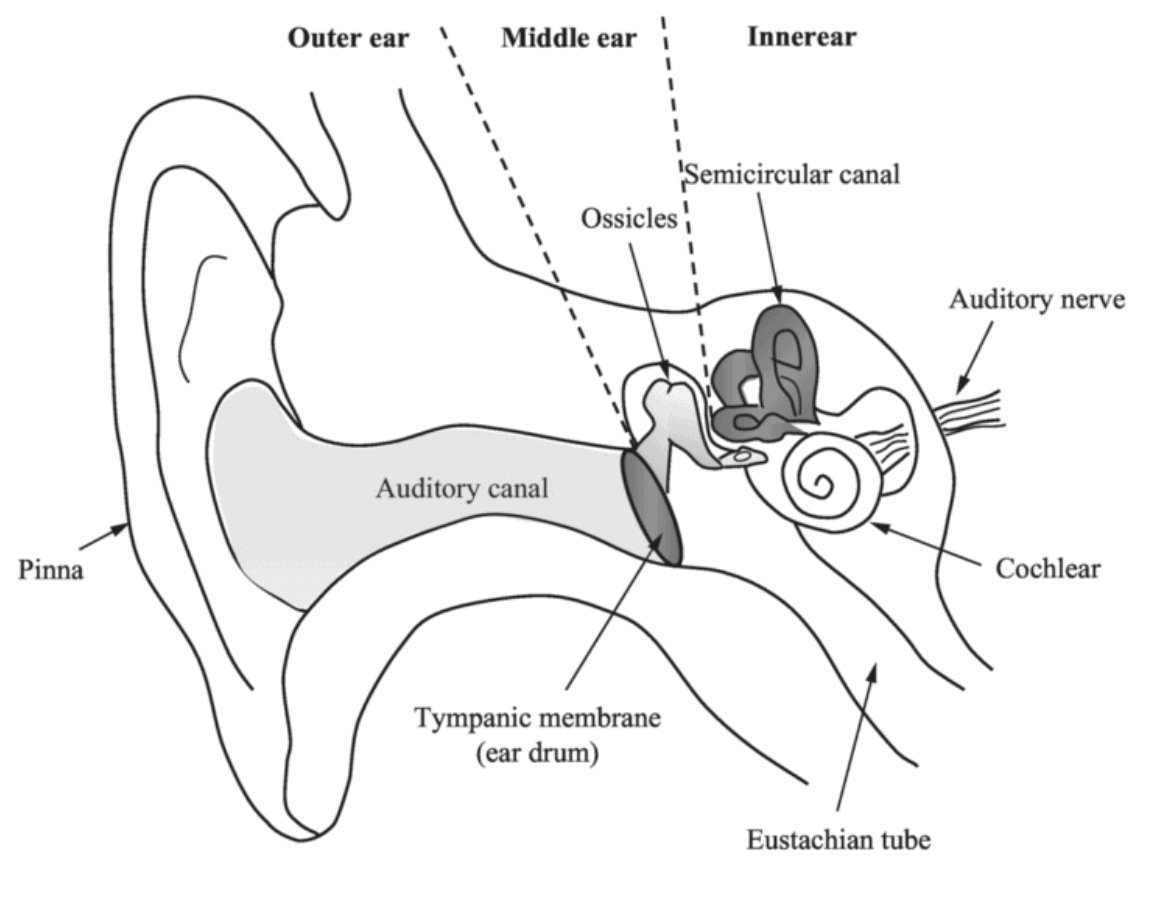
\includegraphics[width=0.5\textwidth]{wayland-ear}
   \caption{The external, middle and the inner ear from \citet{Wayland2018Phonetics}}
   \label{fig:ear}
\end{figure}

\subsubsection{The Outer Ear}
The outer ear (sometimes referred to as the External Ear) is responsible for channeling sound waves to the tympanic membrane (ear drum). Firstly,
sound waves reach the Pinna (the part of the ear that we can see and touch), which funnels it through the auditory canal, and at the end of the canal 
is the ear drum, at which point the sound waves collide with the eardrum, which causes the eardrum to vibrate. 
The vibrations are passed through the middle ear.

\subsubsection{The Middle Ear}
Zooming into the middle ear (Figure \ref{fig:middle-ear}), there are three bony structures: the Malleus, Incus, and Stapes,
and together they make up a lever system. 
It is worth pointing out that when energy is transmitted from the eardrum to the middle ear, there is bound to be some energy loss which can be as high as 40\%. The lever system's mechanical advantage 
allows for the sound energy to be amplified, so the loss of energy is compensated. 

The Stapes also has an additional function in addition to passing over the sound vibrations to the inner ear. That is,
the Stapes is connected by a muscle, the Stapedius muscle, and in response to loud noises, it temporarily increases the stiffness of the bones in the middle ear, which temporarily prevents the acoustic energy from being amplified. This 
protects the inner ear from loud noises.

\begin{figure}[h]
   \centering
   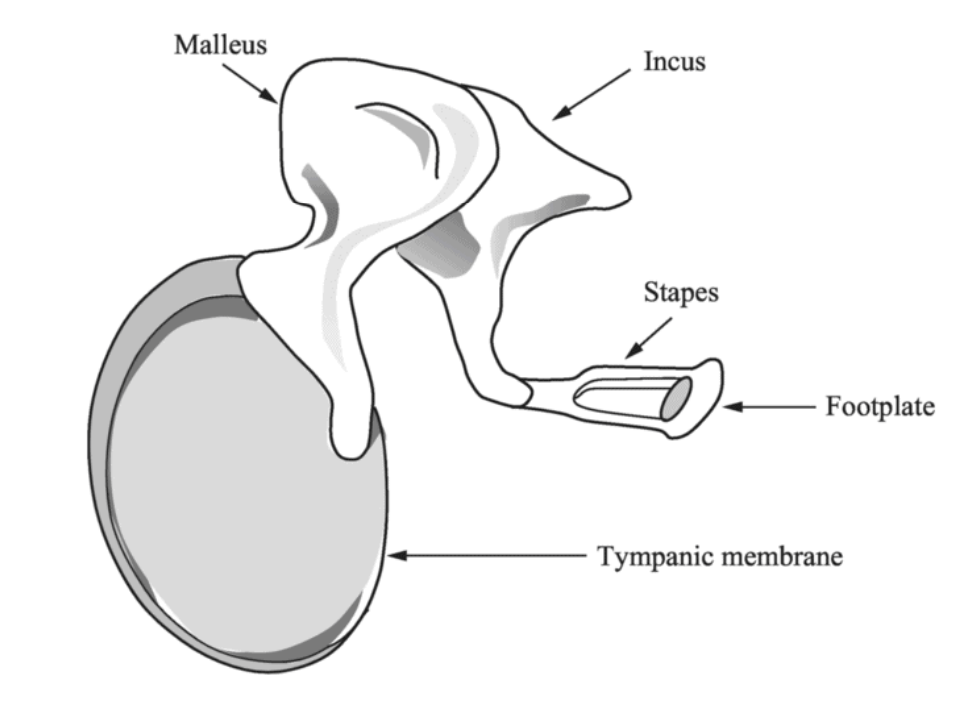
\includegraphics[width=0.5\textwidth]{wayland-middle-ear.png}
   \caption{The components of the middle ear from \citet{Wayland2018Phonetics}}
   \label{fig:middle-ear}
\end{figure}

\subsubsection{The Inner Ear}
One of the parts of the inner ear is the Cohlea, which gives humans the ability to hear sounds.
The Cochlear is a bony structure that resembles that of a snail shell \footnote{'Cochlear' in Latin translates to snail shell!}.
If the Cochlear was unrolled its length would be about 3.5cm, and it is subdivided into various parts (see Figure \ref{fig:cohlear}).
For our purposes, it suffices to know that in the Basilar membrane is a collection of cells, called 
the Organ of Corti, which contain hair cells, and that different hair cells register different frequencies.
Figure \ref{fig:corti} shows the frequency responses and the various areas of the corti 
and its response to different frequencies. The Organ of Corti is linked to the auditory nerves and 
so the oscillations that pass through it get converted to neural impulses and transmitted to the brain.

\begin{figure}[h]
   \centering
   \begin{minipage}{0.4\textwidth}
      \centering
      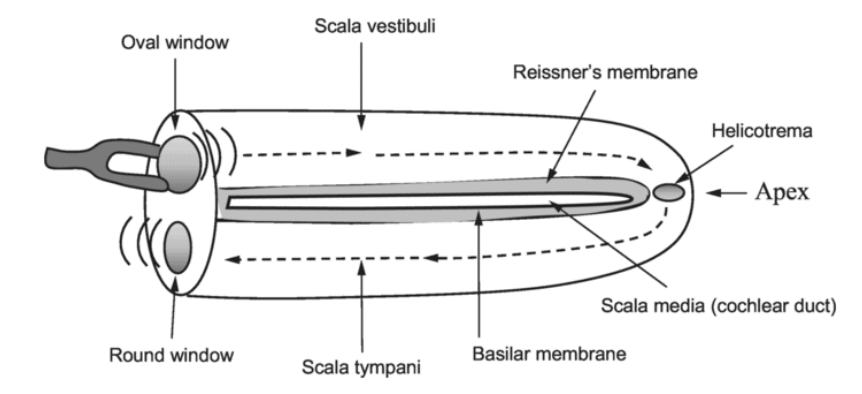
\includegraphics[width=\textwidth]{wayland-cohlear.png}
      \caption{'Unrolled' Cochlear from \citet{Wayland2018Phonetics}}
      \label{fig:cohlear}
   \end{minipage}
   \hfill
   \begin{minipage}{0.48\textwidth}
      \centering
      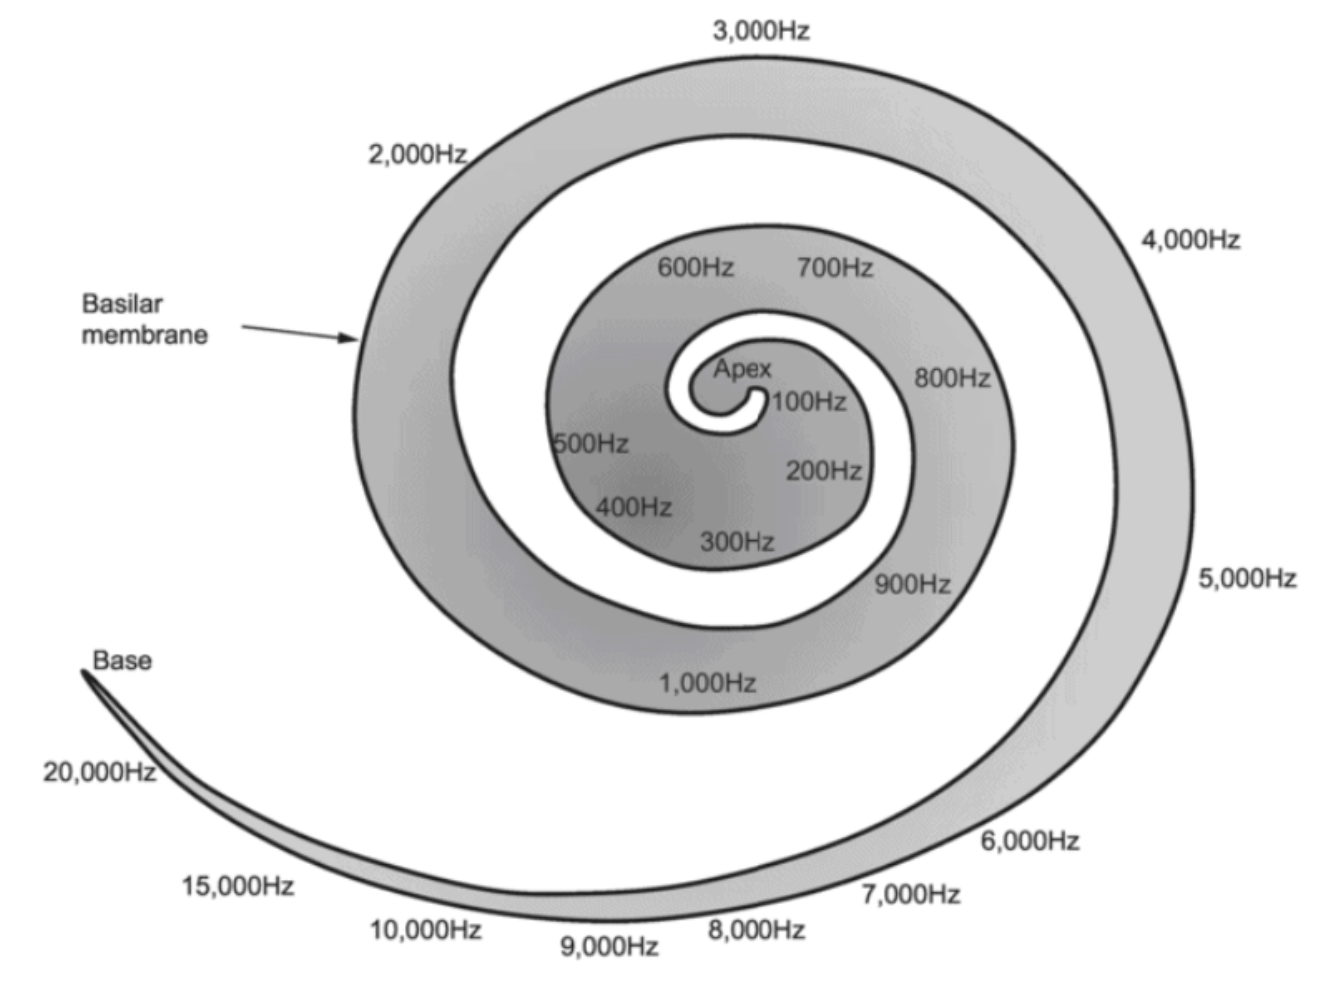
\includegraphics[width=0.5\textwidth]{wayland-corti-2.png}
      \caption{The Organ of Corti and the frequency responses. From \citet{Wayland2018Phonetics}}
      \label{fig:corti}
   \end{minipage}
\end{figure}

% \subsection{Congenital Hearing Loss}
% TODO
% \subsection{Exposure to Loud Noises}
% TODO
% \subsection{Ageing}
% TODO
\subsection{Hair Cell Loss and Hearing Loss}
As we have seen, hair cells play a major role in allowing humans to register sound. Unfortunately,
it is the main cause of hearing loss, as those hair cells are susceptible to damage.
The cause of hair cell loss is complex since it could be due to many factors such as 
genetic abnormalities (congenital hearing loss), infection, diseases, or extrinsic factors such as exposure to loud noises.
It can also occur due to ageing, which could be due to the reasons mentioned above, but could also be triggered due to age-related hearing loss genes. To make matters worse, hair cell loss is unrecoverable in humans \citep{Furness2015HairCell}.
Hearing loss is a spectrum and varies from mild (26-40dB loss), moderate (41-60dB loss), severe (61-80dB loss) to profound($>80$dB loss) \citep{Nieman2020HearingLoss}.
In addition, hearing loss can occur in one ear (unilateral) or in both ears (binaural). 

\section{Hearing Loss Treatment}

We now know how the auditory system works and how hearing loss can occur.
Hearing solutions have come a long way, 
from acoustic devices to modern digital devices. 
As this dissertation is focused on 
the incorporation of machine learning techniques into hearing aids,
we will gloss over the history of acoustic devices, but 
for a comprehensive overview of the history of hearing technology,
refer to the paper by \citet{levitt_historical_2007}.

% \subsection{History of Hearing Technology}
% TODO: Will see how much pages I have left after doing other chapters.

% Users were fitted with what would have been considered a HA in this day and age as early as the 18th century.


\subsection{Hearing Technology}
As mentioned in the Introduction, the most common treatment for hearing loss 
is the provision of hearing technology. There are two common approaches 
to the fitting of hearing technology: the equipment of a Hearing Aid (HA) 
or the fitting of a Cochlear Implant. There are similarities between the 
two, and both can be used to fit users who experience profound hearing loss, 
although Cochlear implants are only considered if the user is experiencing 
a severe hearing loss or more. While we 
focus on the HA, the concepts we explore can be applied to the CI.
The components of a HA vary widely, but at least, 
it contains a microphone, amplifier, receiver, and battery \citep{schuster-bruce_conventional_2025}.
A microphone is a device that converts acoustic sound waves into electrical signals. 
The electrical signals are then amplified by the amplifier, and the receiver converts the electrical 
signals back into acoustic waves. The battery is used to power the device. 
Depending on the user, they may be fitted with a hearing aid in each 
ear (binaural) or a single hearing aid in one ear (unilateral). 
Typically, the hearing aid contains multiple microphones and the microphones 
are placed in different locations on the device. 
% Figure \ref{fig:hearing-aid} shows an image 
% of a hearing aid.


\subsection{Hearing Technology Now}

% Recent advances in hearing aid technology have led to the integration of increasingly sophisticated signal processing algorithms, including deep neural networks (DNNs) and artificial intelligence (AI), to enhance auditory performance and overall quality of life for users.
% High-profile innovations, such as Apple's FDA-approved AirPods and developments from established manufacturers like Phonak and Oticon, exemplify this trend with the incorporation of DNN-based processing techniques.

% A notable development is the shift towards rechargeable hearing aids that utilise lithium-ion batteries.
% These devices not only offer the practical benefit of eliminating battery replacement but also support higher peak power consumption, thereby accommodating the computational demands of advanced models such as DNNs.
% In contrast, hearing aids powered by zinc-air batteries remain limited by the intrinsic energy constraints of their power source.
% Recent studies report that under high power conditions, the average battery life of non-rechargeable, zinc-air-powered hearing aids lies within the range of 50–80 hours \citep{sparkes_study_1997, mir_evaluation_2023, thomas_zincair_2024}.
% Rechargeable devices typically achieve operational durations of 15–30 hours, and when features like Phonak's Speech Enhancer are activated in noisy environments, maximum battery life can drop to below six hours.


% These findings underscore a fundamental trade-off in hearing aid design: while the application of DNNs can significantly elevate the performance of auditory devices, it concurrently imposes strict energy requirements that may compromise battery longevity.
% Future research should therefore focus on optimising power efficiency to better balance computational performance with practical usability.

As discussed in the Introduction, the increasing demand for HAs is driving not only 
the development of more sophisticated HAs, but also the entry of big tech 
companies like Apple to the hearing aid market, and the developments from established 
manufacturers like Phonak who are starting to incorporate DNNs into their devices.

Another trend is that of the shift towards rechargeable hearing aids (Lithium Ion Batteries).
These devices offer not only the practical benefit of eliminating battery replacement, but also support higher peak power consumption, which could explain the correlation in the sudden interest in using DNNs in HAs.
In contrast, hearing aids before the transition to rechargeable hearing aids were using Zinc-air batteries 
(\cite{sparkes_study_1997}; \cite{mir_evaluation_2023})
that are non-rechargeable.
A recent study by \citet{thomas_zincair_2024}, which 
experiments with various Zinc-air manufacturers, shows that the average battery life 
under high-power conditions is 50-80 hours. Contrast this with the average battery life of 
rechargeable hearing aids which is typically in the region of 15-30 hours and 
features such as Phonak's Speech Enhancer (the DNN based feature) can drop the battery life 
to below 6 hours. 

These findings highlight an important trade-off in hearing aid design. While there is lot of potential to improve the performance of HAs (DNNs or otherwise),
it can come at the cost of battery life and possibly constrains 
the types of model that can be used. 

Due to the proprietary nature of the devices, it is unclear what kind of 
algorithms are used on the devices. However, from Phonak's white paper on Spheric Speech Clarity \cite{Hasemann2024PhonakSphere}
we can deduce that the devices use a combination of ASA and speech enhancement techniques.
From the paper, before signal processing begins, the sound is fed into Autosense OS which 
performs `scene classification' so in the context of this project, this can be 
considered as an acoustic scene analysis (ASA) algorithm. More specifically, if 
the signal is classified as 'Speech in Loud Noise', then the signal is fed into a 
deep neural network which outputs a mask that separates the speech signal from the background noise 
which is then applied to the signal. 



% It is enough 
% to know for now that the devices will contain multiple microphones, and 
% a dedicated chip which does further processing on the sound depending 
% on the environment the user is faced with.
% It should be pointed out that there is an active area 
% of research into curing congenitial hearing loss - individuals who have been diagnosed with 
% a hearing loss since birth.
% \subsubsection{Hearing Aids}
% Figure ... shows a typical hearing aid, and Figure ... shows the hearing aid labelled.
% TODO
% Microphone info, the reason for multiple mics etc
% There is a surge into rechargable hearing aids.
% Smaller model = higher battery life 

% \subsection{New Approaches to Treatment}
% \subsubsection{Gene-Based Therapy}
% Genitic mutations account for 70-75\% of congenital hearing loss, and with the advent 
% of gene-based therapy, it is not surprising to see that this avenue is explored with hearing loss. 
% However, besides it being an active area of research, it will not be applicable 
% to individuals that have 

\newpage
\section{Speech Processing Techniques}
\subsection{Digitisation}
\begin{figure}[h]
   \centering
   \includegraphics[width=\textwidth]{waveform-spectrogram.png}
   \caption{A waveform (bottom) and its spectrogram (top). 
   We used an excerpt mixed with speech with the `InTraffic'
   environment from the HEAR-DS dataset \citep{Huwel2020HearDS}.}
   \label{fig:waveform-spectrogram}
\end{figure}
To be able to perform speech processing on a device containing a chip/processor such as a HA, requires us 
to have some sort of digital representation of the sound wave. A waveform is just that, a digital representation 
of the sound we hear [Figure \ref{fig:waveform-spectrogram}]. A microphone is a device that converts those sound waves into a representation of the 
waveform. Conceptually, this is done by measuring the relative air pressure at different points in time, and 
this is represented as a waveform or a time series of amplitudes. Digital devices cannot have infinite precision, so the signal produced by the sound will 
be divided into discrete samples, and the rate at which this occurs is known as the sampling rate. Additionally,
the precision of the amplitude of the signal will be quantized into discrete numbers, and the precision is 
dictated by the bit depth (or the quantization rate).

The selection of these two parameters is determined by the nature of the speech task and the Nyquist-Shannon Sampling Theorem.
This theorem states that the sampling rate should be at least twice the highest frequency present in the signal. 
That is, for a signal containing frequencies up to 8KHz, the minimum required sampling rate would be $f_s \ge 16$KHz.
Otherwise, aliasing will occur, which is the phenomenon in which high-frequency components could be misinterpreted as lower frequencies,
which could be undesirable in both tasks we are trying to perform. Typically, datasets will have a sampling rate 
of 44KHz, and, generally, for ASA tasks, a sampling rate of 16KHz is acceptable. 
With regard to bit depth, it is selected based on the dynamic range required to capture speech signal variations. 
Commonly, 16-bit depth is used, which is capable of representing an amplitude range of approximately 96dB, thereby ensuring sufficient resolution in amplitude representation.

\subsection{Engineered Acoustic Features}
The prevalence of engineering acoustic features in previous work related to my project and speech processing in general
warrants a high-level overview of this concept to better understand its usage. 
Given some signal $x(t)$, an engineered feature $\phi(x(t))$ is a function that transforms the signal in some way.

In this project, we will be working with spectrograms, which are a type of engineered feature.
To obtain the spectrogram, we first need to convert the signal (waveform) into the frequency domain (Figure \ref{fig:waveform-spectrogram}).
The process of converting the signal into the frequency domain is done by utilising 
the Fourier Transform. We will technically be using the Short-Time Fourier Transform (STFT) 
due to efficiency, and the main hyper-parameters for the STFT are the window length $w$ 
and the hop length $h$. The window length is the length of the window that is used to 
split the signal into frames, and the hop length is the number of samples between the 
start of each frame. Additionally, there is a choice of a window function and we will 
be using the most common one, the Hann window. Once we apply the STFT, we will be 
left with a complex-valued vector of length $w$ and the magnitude of this vector 
gives us the amplitude of the signal at different frequencies. 

From there, various transformations can be applied to the spectrogram 
to enhance its suitablity for specific tasks. For the ASA task, we utilise the 
log-mel spectrogram, which is obtained by applying a Mel Filterbank to the spectrogram 
and taking the logarithm of the outputs, which mimics the human perception 
of loudness and is a popular choice in the speech processing literature. 
For SE, the conventional spectrogram is used by popular choice in the speech enhancement literature.

These engineered acoustic features offer a compact representation of the signal, thereby 
reducing memory and computational demands, which is crucial for embedded devices such as 
HAs, and they often enhance the distinction between speech and background noise, 
which is a desirable property for speech processing tasks such as ASA and SE.
\section{Related Work}
As this project will chain two algorithms: Acoustic Speech Analysis and Speech Enhancement, 
to form a state-dependent model, we will briefly cover the related work for each task.
Additionally, we will cover the idea of Green AI and how it can be applied to the development of the models.

\subsection{Acoustic Scene Analysis}
% TODO: Talk aobut why neural approach is better than classical maybe 
We will give a more mathematical formulation of the ASA task in section \ref{sec:methodology-asa}. 
But conceptually, the task is to classify an input signal into one of the pre-defined scenes/classes.

Typically, the two approaches to ASA operate 
in the frequency domain or the time domain, otherwise known as end-to-end models, 
since they operate in the raw waveform directly. 
There is an equal amount of research on both approaches, 
such as the articles by \citet{schindler_multi-temporal_2018} and \citet{kim_specmix_2021} 
in the former case (frequency domain) and \citet{dai_very_2016} 
and \citet{kumar_end_2020} in the latter case (time domain).

A novel dataset was developed in response to the inadequacies of existing ASA databases for HA processing. 
This dataset was developed by \citet{Huwel2020HearDS} and is called the HEAR-DS dataset (for more details, see Chapter \ref{sec:datasets}).
The original paper on the HEAR-DS dataset illustrates its applicability by employing a Convolutional Neural Network (CNN) for ASA in the frequency domain. 

While in this part of the dissertation we will be using the frequency domain approach,
we will be exploring the time domain approach in part 2 of this dissertation. 
The motivation for this is to determine whether the overhead of constructing engineered features is too high compared to operating on the raw waveform. 
Alternatively, the increased input dimensionality may counterbalance this overhead. Future research should explore this trade-off from an HA perspective.
% There is also a compendium of ASA challenges occuring in the literaturem such 
% as the DCASE 2017 Acoustic Scenes Challenge \citep{DCASE2017challenge}, where 
% researchers such as \citet{schindler_multi-temporal_2018} have participated in the challenge 
% to improve the state-of-the-art in ASA.
%  The two papers mentioned above utilise engineered features, and more specifically, the log mel spectrogram. 
% While operating on the time domain is not explored in this part of the dissertation, it is something I will be looking into 
% in part 2 of this dissertation as the overhead of the Fourier Transform and the Mel Filterbank in a hearing aid 
% is potentially too high, and so working directly with the waveform may be a more feasible approach. 


% The challenges encountered during this replication process are discussed comprehensively in the chapter. 

% % Additionally, to validate the model implementation, the same parameters were applied to the DCASE 2017 Acoustic Scenes Challenge dataset \citep{DCASE2017challenge}. In particular, a comparison is drawn between the model proposed by \citet{schindler_multi-temporal_2018} and the CNN model used in the HEAR-DS paper, with the findings detailed in Section \ref{sec:DCASE-results}.
% The two papers mentioned above utilise engineered features, and more specifically, the log mel spectrogram. This 
% approach in some literature is called operating on the frequency domain. It is worth pointing out 
% that there is research into doing ASA on the time domain i.e. operating on the waveform directly, 
% such as the papers by \cite{dai_very_2016} and \cite{kumar_end_2020}. While not explored in this part, 
% it is something I will look into exploring in part 2 of this dissertation as there is 
% a compelling reason to possibly consider the time domain approach. Namely, 
% the overhead of the Fourier Transform and the Mel Filterbank in a hearing aid 
% is potentially too high, and so working directly with the waveform may be a more feasible approach.

% TODO: VERY DEEP CONVOLUTIONAL NEURAL NETWORKS FOR RAW WAVEFORMS

\subsection{Speech Enhancement}
On the other hand, Speech Enhancement aims to improve the perceptual quality of a speech signal that 
has been degraded by additive noise \citep{loizou_speech_2007}. 
This enhancement is crucial in applications where speech intelligibility is essential, such as telecommunications, hearing aids, and speech recognition systems. Noise sources may include environmental disturbances (e.g., wind noise) as well as interference from multiple speakers (e.g., babble noise).

% TODO: Talk about why we are using a neural-network based approach
There are many different approaches to speech enhancement, from more traditional methods such as spectral subtraction, or Wiener filtering
to more modern methods that incorporate neural networks. In this dissertation, we will be using a neural network based approach.
But even within the neural network-based approach, there are different techniques that can be used to enhance the speech signal. 
Neural network-based speech enhancement algorithms are categorised into four primary types \cite{katagiri_handbook_2000}:
\label{sec:se-methods}
\begin{itemize}
   \item \textbf{Time-Domain Filtering} - Trains a neural network with noisy inputs (background + speech) and clean targets (speech only). 
   This involves working with the waveform directly; however, it is not without its challenges and is still an active area of research \citep{saleem_time_2024}.
   \item \textbf{Transform-Domain Filtering} - Trains a neural network with noisy inputs (background + speech) and clean targets (speech only). 
   The difference between this and the Time-Domain Filtering approach is that the input is transformed into the frequency domain 
   (whether that be a Fourier transform, or a Mel Spectrogram, Mel-Frequency Cepstral Coefficients (MFCCs), LPC, etc.). The advantage of this 
   is that the dimensionality of the input is usually lower, and the representation is more robust to separation of the speech and background noise.
   This is also a popular approach in the literature on speech enhancement \citep{tan18_interspeech,hou_local_2023}.
   \item \textbf{State-Dependent Model Switching} - The two mentioned approaches assume that the speech signal and noise source are stationary. 
   This is too strong an assumption, and so state-dependent model switching is a paradigm that has been explored. The main idea is 
   to have a class of models, each specialising in handling a different type of noise, and to switch between them based on the characteristics of the input signal. This in a way is the chaining of ASA and Speech Enhancement, as the ASA model will first classify the input signal into a state, and then the appropriate speech enhancement model will be selected and applied to the signal.
   To our knowledge, this technique in the context of HAs has not been discussed in the literature, but it 
   appears to be implemented in state-of-the-art HAs. 
   \item \textbf{Online Iterative Methods} - The focus is on incorporating adaptive techniques that do not rely on pre-existing 
   training data. Key approaches include adaptive predictors, dual EKF (Extended Kalman Filter) algorithms, and noise-regularised adaptive filtering.
   There is some active research into the incorporation of Kalman Filters (KFs) or EKFs into the neural pipeline for speech enhancement \citep{Xue2020NeuralKF, Mellahi2023SpeechEU}.
\end{itemize}
The discussion of the engineering of acoustic features in the previous section is relevant here, as the Transform-Domain Filtering approach
is what will be used in this part of the dissertation. 
Then, the main contribution of this dissertation is the exploration of 
the feasibility of state-dependent model switching in the context of HAs. 
Given that it seems to be already used in state-of-the-art HAs, it 
would be a good idea to formalise this approach in the literature 
so that potentially future work can build on this.


% Though, exploring the time domain approach is something I will be looking into for the second part of this dissertation 
% due to the potential overhead reduction of the time domain approach as mentioned in the previous section.

\subsection{The parallels of Green AI}
The paper by \citet{schwartz2019greenai} discusses the idea of Green AI 
which is to advocate for the use of hardware-independent performance metrics.
Metrics such as electricity consumption or elapsed real-time are not good metrics 
as they are dependent on the hardware on which the model is run. 
Although the number of parameters in a model has been proposed as an 
alternative metric, it can be problematic when comparing different model architectures, 
since it is possible that despite a more complex model having more parameters, 
it could compute the same amount of work in a more efficient manner. 

Instead, \citet{schwartz2019greenai} discusses how the number of floating point operations [FLOP(s)]
provides a more concrete and meaningful measure of computational workload. 
FLOP(s) are computed by analytically counting the number of \texttt{ADD} and \texttt{MULT} operations in the model.
This is effective, as all operations in a DNN can be recursively reduced to a combination 
of \texttt{ADD} and \texttt{MULT} operations.
As an added bonus, the fact that we have insight into HA's potential FLOPs is useful 
as it allows us to compare the model's performance to the hardware's potential. If our
models are using less FLOP(s) than a HA device, then we know that the model is
potentially more energy efficient or that we could investigate expanding
the model. On the flip-side, if the model is using more FLOPs than a HA device, 
then we know that the model is potentially too large for a HA device and we need
to look for ways to reduce the model size. It also helps that there is load
of literature on reducing the FLOP(s) of DNNs (e.g. \cite{liu_simple_2023}), so
using FLOP(s) as a metric is good not only from a reproducibility standpoint, 
but from a development standpoint as well. 

\section{Criticism of Previous Work}
\label{sec:criticism}
\subsection{Acoustic Scene Analysis}
In the ASA field, we will predominantly be using the HEAR-DS dataset introduced by \citet{Huwel2020HearDS}
and a major part of this dissertation is to analyse and explore the model in more detail.
The motivation behind the further exploration and analysis of the model is due
to the gaps in the analysis of the paper. Granted, the paper was more of an exploration of the applicability of the dataset 
and so more `verbose' evaluations were not the scope of the paper. 
Additionally, as will become clear, the reproduction of the results 
was difficult, and while we had to deviate from the paper's approach
in some aspects, in other cases, we had to make some assumptions
about the pipeline details of the paper. 
In the following we outline some of the issues we found with the paper.
\begin{itemize}
   \item \textbf{Controlling for Imbalanced Dataset} - The lack of explanation on the data splitting strategy 
   is a cause of concern, since as will become clear in Chapter \ref{chap:asa-experiments},
   the dataset is going to be severely imbalanced. As such, metrics such as accuracy are not going to be a good 
   indicator of the model's performance. We will be extending the evaluation of the models to include 
   precision, recall and F1 scores to get a more holistic view of the model's performance. 
   \item \textbf{Claim on SGD Optimiser} - The paper claims that the Stochastic Gradient Descent (SGD) 
   optimiser was used over the Adam optimiser due to the sensitivity of the Adam optimiser in 
   initialisation. They cite this with a paper by \citet{Reddi2019convergenceadam},
   but after reading it, while it says 
   Adam can lead to poor convergence in `\textit{some settings}',
   thus it would have been insightful to see from \citet{Huwel2020HearDS}
   if this is the case for the ASA task.
   \item \textbf{Feasibility} - Furthermore, given that 
   this is a dataset tailored for HA research, it would have been insightful 
   to see the feasibility of the models when used in a HA device. While the paper 
   reports the elapsed real-time of the models, this
   is inadequate due to the hardware-dependent nature of the metric. 
   We will be reporting FLOP(s) and number of parameters to provide a more 
   concrete and meaningful metric of the model's performance as per \citet{schwartz2019greenai}.
\end{itemize}
It is important to note that the intention is not to 
be critical of the valuable work done by the original authors 
but rather to bring more insight that was built from the work of the original authors.
This is done by providing a deeper insight into the model's performance 
and feasibility when used in an HA device. The challenges encountered 
in reproducing the results underscore the need for more 
detailed methodological documentation, and so this dissertation aims 
to address this gap. We also want to take the author's 
mission further and explore other use-cases of the dataset, 
such as the task of Speech Enhancement and how the two tasks 
(ASA and SE) can be combined to form a state-dependent model,
all within the context of a HA device.
\newpage

\subsection{Speech Enhancement}
Although the \heards dataset has not previously been employed 
for SE, this dissertation investigates its potential in this domain.
Our methodology is inspired by the paper by \citet{tan18_interspeech}
who presented a convolutional encoder-decoder (CED) model.
Despite the claim of `real-time speech enhancement', the paper 
lacks an evaluation on the model's real-time inference capabilities 
and does not address the feasibility of the model in a HA device. 
Given that HA applicability was mentioned as part of their abstract,
it appears that the original authors were at least partially 
aware of the potential of the model in such contexts. However, 
no further elaboration was given in the paper. 

This is a common trend in the SE literature, where multiple papers
introduce SE models that highlight applications for HAs without 
thoroughly discussing the computational constraints of HA devices. 
Although recent publications \citep{DuSpiking2024,Sach2023EffCRNAE,Wang2025ZipEnhancerDD} 
have begun reporting FLOP(s) as a measure of model complexity,
they exhibit two significant limitations. Firstly, they do not utilise HA-specific datasets 
such as \heards. Secondly and more importantly, to the best of our knowledge
none of these studies compare the model's FLOPs to the computational capacity 
of HA devices, leaving a critical gap in assessing practical feasibility. 
This dissertation aims to bridge this gap by introducing an approach 
for evaluating the feasibility of SE models on HA devices, informed by 
recent insights into their computational constraints.



% Additionally, there is much less discussion of SE models when considering multiple 
% environments, which could be due to limited datasets that cover a wide range of environments 


% In summary, while the previous study makes a valuable contribution
% to the field of HA research, a more thorough and systematic
% evaluation is necessary to fully assess the model's efficacy 
% in the task of ASA. This dissertation aims to contribute 
% to that venture by offering a comprehensive analysis
% of the model under conditions that more closely mirror real-world HA applications.
% Additionally, we want to take the paper's mission further and explore 
% other use-cases of the dataset, such as the task of Speech Enhancement 
% and how the two tasks (ASA and SE) can be combined to form a state-dependent model,
% all within the context of a HA device.

% and CHiMe 5 \cite{barker18_fifth_2018} datasets. However, only the CHiME 3 development set was used for mixing the speech into the background noise.
% CHiME 5 was used for creating a new environment, 'Interferring Speakers', which are samples that contain speech from multiple speakers.
% I think using the CHiME 3 dataset and especially only the development set was an odd decision, as there is only roughly 10 hours of data 
% from 4 speakers. So a model trained on this dataset may not generalise well to real world scenarios, due to the rich variability of 
% speech from different speakers. Nevertheless, we continue with the paper's approach to set up a baseline. Another odd decision was 
% in the use of a fixed learning rate scheduler, and the use of a high epoch count without what appears to be no early stopping. This 
% will be discussed in more detail in Chapter \ref{chap:asa-experiments}. We still thank the authors for their work on the dataset 
% as it is a promising dataset for the future of HA research. Additionally, given that the dataset 
% has the potential to be used for HA devices, there is not any mention on the viability of the models 
% when used in a HA device. So a significant aspect of this project is to investigate the feasibility of 
% incorporating a DNN model into a HA device. 


\chapter{Methodology}
\label{chap:methodology}

% The model presented in the paper assumed a sampling rate of 16KHz, so we resampled the HEAR-DS dataset to 16KHz. Additionally, 
% the model expected a log-mel spectrogram of 10s segments, and the HEAR-DS dataset provided longer segments. We therefore 
% split the HEAR-DS segments into 10s segments by traversing the dataset and extracting 10s segments. There is potential 
% for this to have discontinuities in the beginning and end of the segments, but from the paper it is unclear how this 
% was addressed if at all. We went with a naive approach of just cutting the segments.


\section{Acoustic Scene Analysis}
\label{sec:methodology-asa}
Mathematically, ASA can be formalised as follows:
Consider an audio signal \(x \in \mathbb{R}^{T}\), where \(T\) denotes the number of samples in the signal, and let \(\mathcal{E} = \{e_1, e_2, \ldots, e_N\}\) represent a set of \(N\) distinct environments. ASA is concerned with determining a mapping 
\[
f: \mathbb{R}^{T} \rightarrow \mathcal{E},
\]
which assigns each audio signal to one of the environments in \(\mathcal{E}\). In this project, \(f\) is implemented as a neural network
and in this first part of the dissertation, we will use a Convolutional Neural Network (CNN) to implement \(f\).

\subsection{Model}
\label{sec:asa-model}
\begin{table}[h]
   \centering
   \begin{tabular}{|c|c|c|c|}
      \hline
      Model & $CNN_1$ & $CNN_2$ & $FC$ \\
      \hline
      net-8 & 8 & 16 & 25 \\
      net-20 & 20 & 40 & 63 \\
      net-32 & 32 & 64 & 100 \\
      \hline
   \end{tabular}
   \caption{Model parameters for the net-X models.}
   \label{tab:cnn-model-params}
\end{table}
As our baseline model, we will use the CNN model presented in the paper by \citet{Huwel2020HearDS}. 
The model has three hyper-parameters: the number of output channels for the first and second convolutional layers ($CNN_1$ and $CNN_2$),
and the number of neurons in the fully connected layer ($FC$). The researchers investigated the effect of different model parameters, 
and in the paper, they train the dataset on 7 different models, where they vary the number of output channels in intervals of 4, thereby training 7 different models.
Due to the time constraints, we will be training 3 models, as we are mostly interested in seeing if we are getting similar results to the paper.
Table \ref{tab:cnn-model-params} shows the parameters of the models we will train.

\begin{figure}[h]
   \centering
   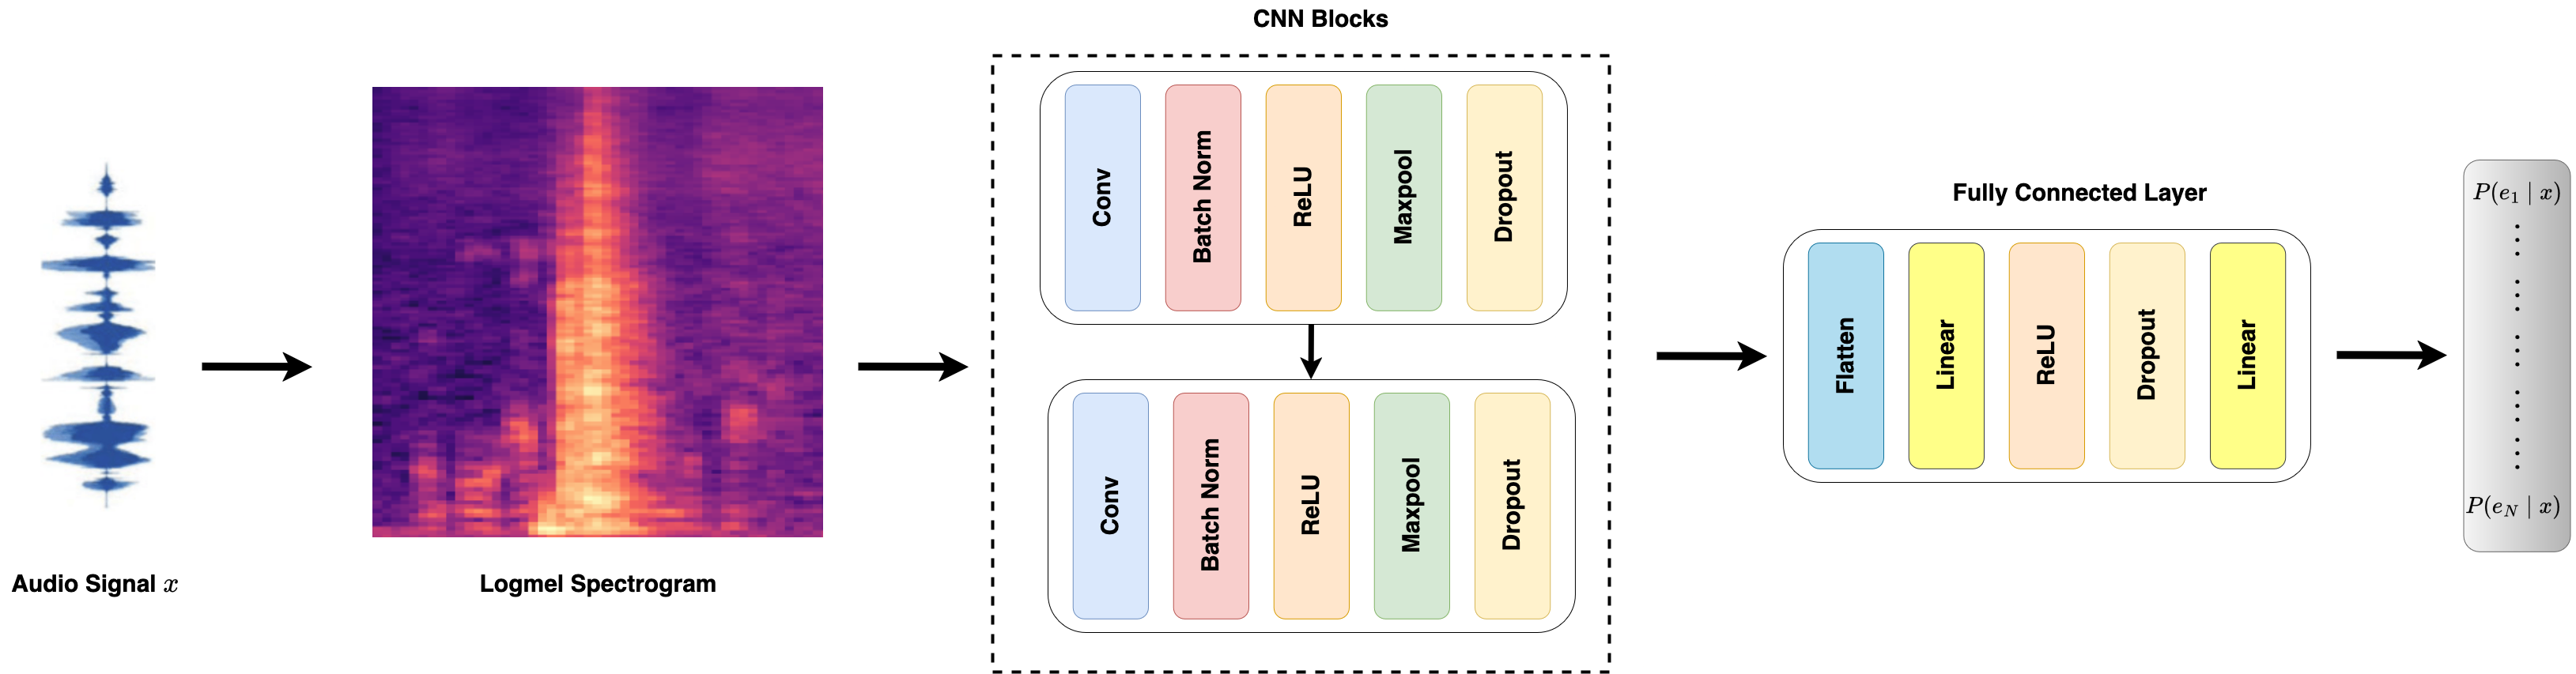
\includegraphics[width=0.95\textwidth]{cnn-diagram2.png}
   \caption{The baseline ASA model architecture.}
   \label{fig:cnn-model-architecture}
\end{figure}
The model architecture is shown in Figure \ref{fig:cnn-model-architecture}. As 
mentioned earlier the models operate on the frequency domain, and 
we stuck with the paper's approach of using a Mel Spectrogram as the 
frequency domain representation for reasons mentioned in the background section. 
According to the paper, all the convolutional layers use a $7 \times 7$ kernel
with a stride of $1 \times 1$ and a padding of $3 \times 3$. After the convolutional operation, 
batch normalisation is applied, which can help with the stability of forward propagation 
and can act as a regulariser which can help prevent overfitting \citep{prince2023understanding}.
The choice of activation function is a Rectified Linear Unit (ReLU) which is computionally 
efficient and reduces the risk of the vanishing gradient problem \citep{prince2023understanding}.
As the preceding operations can increase the dimensionality of the input, a form of down-sampling is applied by using a max-pooling operation, which helps in achieving 
translation invariance and reducing computational complexity for the following layers. Something worth considering for 
part 2 of this dissertation is to explore the use of other down-sampling techniques, and in particular,
\citet{liu_simple_2023} have proposed a family of simple pooling front-ends (SimPFs) 
which in some cases reduce the number of FLOP(s) as much as 75\% in acoustic scene classification tasks. 
Lastly, a dropout of 0.3 is applied after the max-pooling operation which can help with 
the model generalisation \citep{prince2023understanding}.
Applying convolutions is not enough for ASA, 
as we need to have a way to compare the output of the CNN with the set of environments \(\mathcal{E}\).
This is where the fully connected layer comes into play, as it will output a vector of size \(N\), where \(N\) is the number of environments.
The values of the vectors are logits, and so during training and inference, we use a soft-max function to convert them into probabilities.
The soft-max function is defined as follows:
\[
\sigma(x_i) = \frac{\exp(x_i)}{\sum_{j=1}^{N} \exp(x_j)},
\]
where \(x_i\) is the \(i\)-th element of the vector.
The environment with the highest probability is then chosen as the predicted environment, 
that is \(\hat{e} = \arg\max_{e_i \in \mathcal{E}} \sigma(x_i)\).



\subsection{Training}
For ASA, we need a dataset that contains audio signals along with their corresponding environmental labels. 
Mathematically, we need to have a dataset of the form \(\mathcal{D} = \{(x_i, y_i)\}_{i=1}^{N}\), where \(x_i \in \mathbb{R}^{T}\) is the audio signal and \(y_i \in \mathcal{E}\) is the environmental label.
Then a loss function is needed to steer the model towards the correct mapping.
It is important to note that the dataset \(\mathcal{D}\) is not necessarily balanced,
meaning that some environments may have more samples than others.
This is a problem, as the model may learn to classify all samples as the most frequent class. 
So, to combat this, when using a loss function, we apply a weight to each sample based on the number of samples in the dataset.
The weight is defined as follows:
\[
w_i = \frac{n_{samples}}{n_{classes} \cdot n_i}
\]
where \(n_{samples}\) is the total number of samples, \(n_{classes}\) is the number of unique classes, and \(n_i\) is the number of samples in the \(i\)-th environment.
This balanced weighting scheme ensures that the weights sum up to \(n_{samples}/n_{classes}\).
So, a vector of weights \(\mathbf{w} \in \mathbb{R}^{N}\) is created, where \(N\) is the number of environments.
So, we have a vector weight \(\mathbf{w} \in \mathbb{R}^{N}\) that we can use to weight the loss function accordingly.
This is consistent with the paper by \citet{Huwel2020HearDS} where they did ``weighted update steps for each target environment depending on the number of samples in each environment.''
On the topic of the loss function, the paper by \citet{Huwel2020HearDS} does 
not explicitly mention the loss function they used, but we assume that they used the weighted cross-entropy loss function.
The weighted cross-entropy loss function is defined as follows:
\[
L(y, \hat{y}) = -\sum_{i=1}^{N} w_i \cdot y_i \log(\hat{y}_i),
\]
where \(y_i\) is the one-hot encoded environmental label, and \(\hat{y}_i\) is the predicted probability of the model.

Once we have the loss function, we can use it to train the model. There are many approaches to training a model,
and for reproducibility (and as a baseline), we will be using the paper's approach of using Stochastic Gradient Descent (SGD) with a fixed learning rate.
The learning rate was decreased every 40 epochs in a quasi-logarithmic manner: [0.05, 0.01, 0.001, 0.0005, 0.0002, 0.0001].
This leads to a total of 240 epochs of training. 
However, one of objectives of this part of the dissertation was to explore if a different approach to learning rate scheduling
could yield better results. So we will be exploring a different approach to learning rate scheduling in the experiments.
It will be found that the Adam optimiser converges faster than the SGD optimiser and still results in a comparable 
performance. 
\subsection{Evaluation}
The ASA model will be evaluated using the accuracy metric, which is also used by \citet{Huwel2020HearDS}:
\[
Accuracy = \frac{1}{N} \sum_{i=1}^{N} \mathbb{I}(y_i = \hat{y}_i),
\]
where \(N\) is the total number of samples, \(y_i\) is the one-hot encoded environmental label and \(\hat{y}_i\) is the predicted environmental label
and \(\mathbb{I}\) is the indicator function, which is a piecewise function that returns 1 if the condition is true and 0 otherwise.

% However, the issue with accuracy is that taking it 
% at face value can be misleading, even more so in the case of an imbalanced dataset 
% which as will become clear when we discuss the dataset in Chapter \ref{chap:dataset},
% this is certainly the case for the HEAR-DS dataset. 
% So on top of the accuracy metric, we will also be using precision, recall and F1 score metrics.
% These metrics are defined as follows:
Given the imbalanced nature of the HEAR-DS dataset (see Section \ref{sec:hear-ds}),
the accuracy is supplemented with precision, recall and F1 score:
\[
Precision = \frac{TP}{TP + FP}, \quad Recall = \frac{TP}{TP + FN}, \quad F1 = 2 \cdot \frac{Precision \cdot Recall}{Precision + Recall},
\]
where TP is the number of true positives, FP is the number of false positives, and FN is the number of false negatives.
% Intuitively, precision is how well the model is doing at correctly identifying the positive class,
% while recall is how well the model is doing at correctly identifying all positive samples.
% The F1 score is the harmonic mean of precision and recall.

The model performance is further examined across various SNRs to assess robustness
where on the low SNR side, the model may perform poorly because the speech signal being quite faint. 
Conversely, on the high SNR side, the model may perform poorly due to the background noise being quite strong. 


Aligned with the Green AI principles \citep{schwartz2019greenai}, and the ultimate goal of this 
dissertation is to develop models that could be deployed on an HA device, we also evaluate the model 
based on the following: 
\begin{itemize}
   \item \textbf{Floating Point Operations needed for inference [FLOP(s)]} - This will be done by looking at the number of operations the model performs in the forward pass.
   \item \textbf{Theoretical inference time} - Knowing FLOP(s) and FLOP/s we can calculate the theoretical inference time of the model as 
   \begin{equation}
   \text{Theoretical inference time} = \frac{\text{FLOP(s)}}{\text{FLOP/s}}.
   \label{eq:inference-time}
   \end{equation}
   \item \textbf{Number of Parameters} - This will be done by looking at the number of trainable parameters in the model.
\end{itemize}

\section{Speech Enhancement}
\label{sec:methodology-se}
\begin{figure}[h]
   \centering
   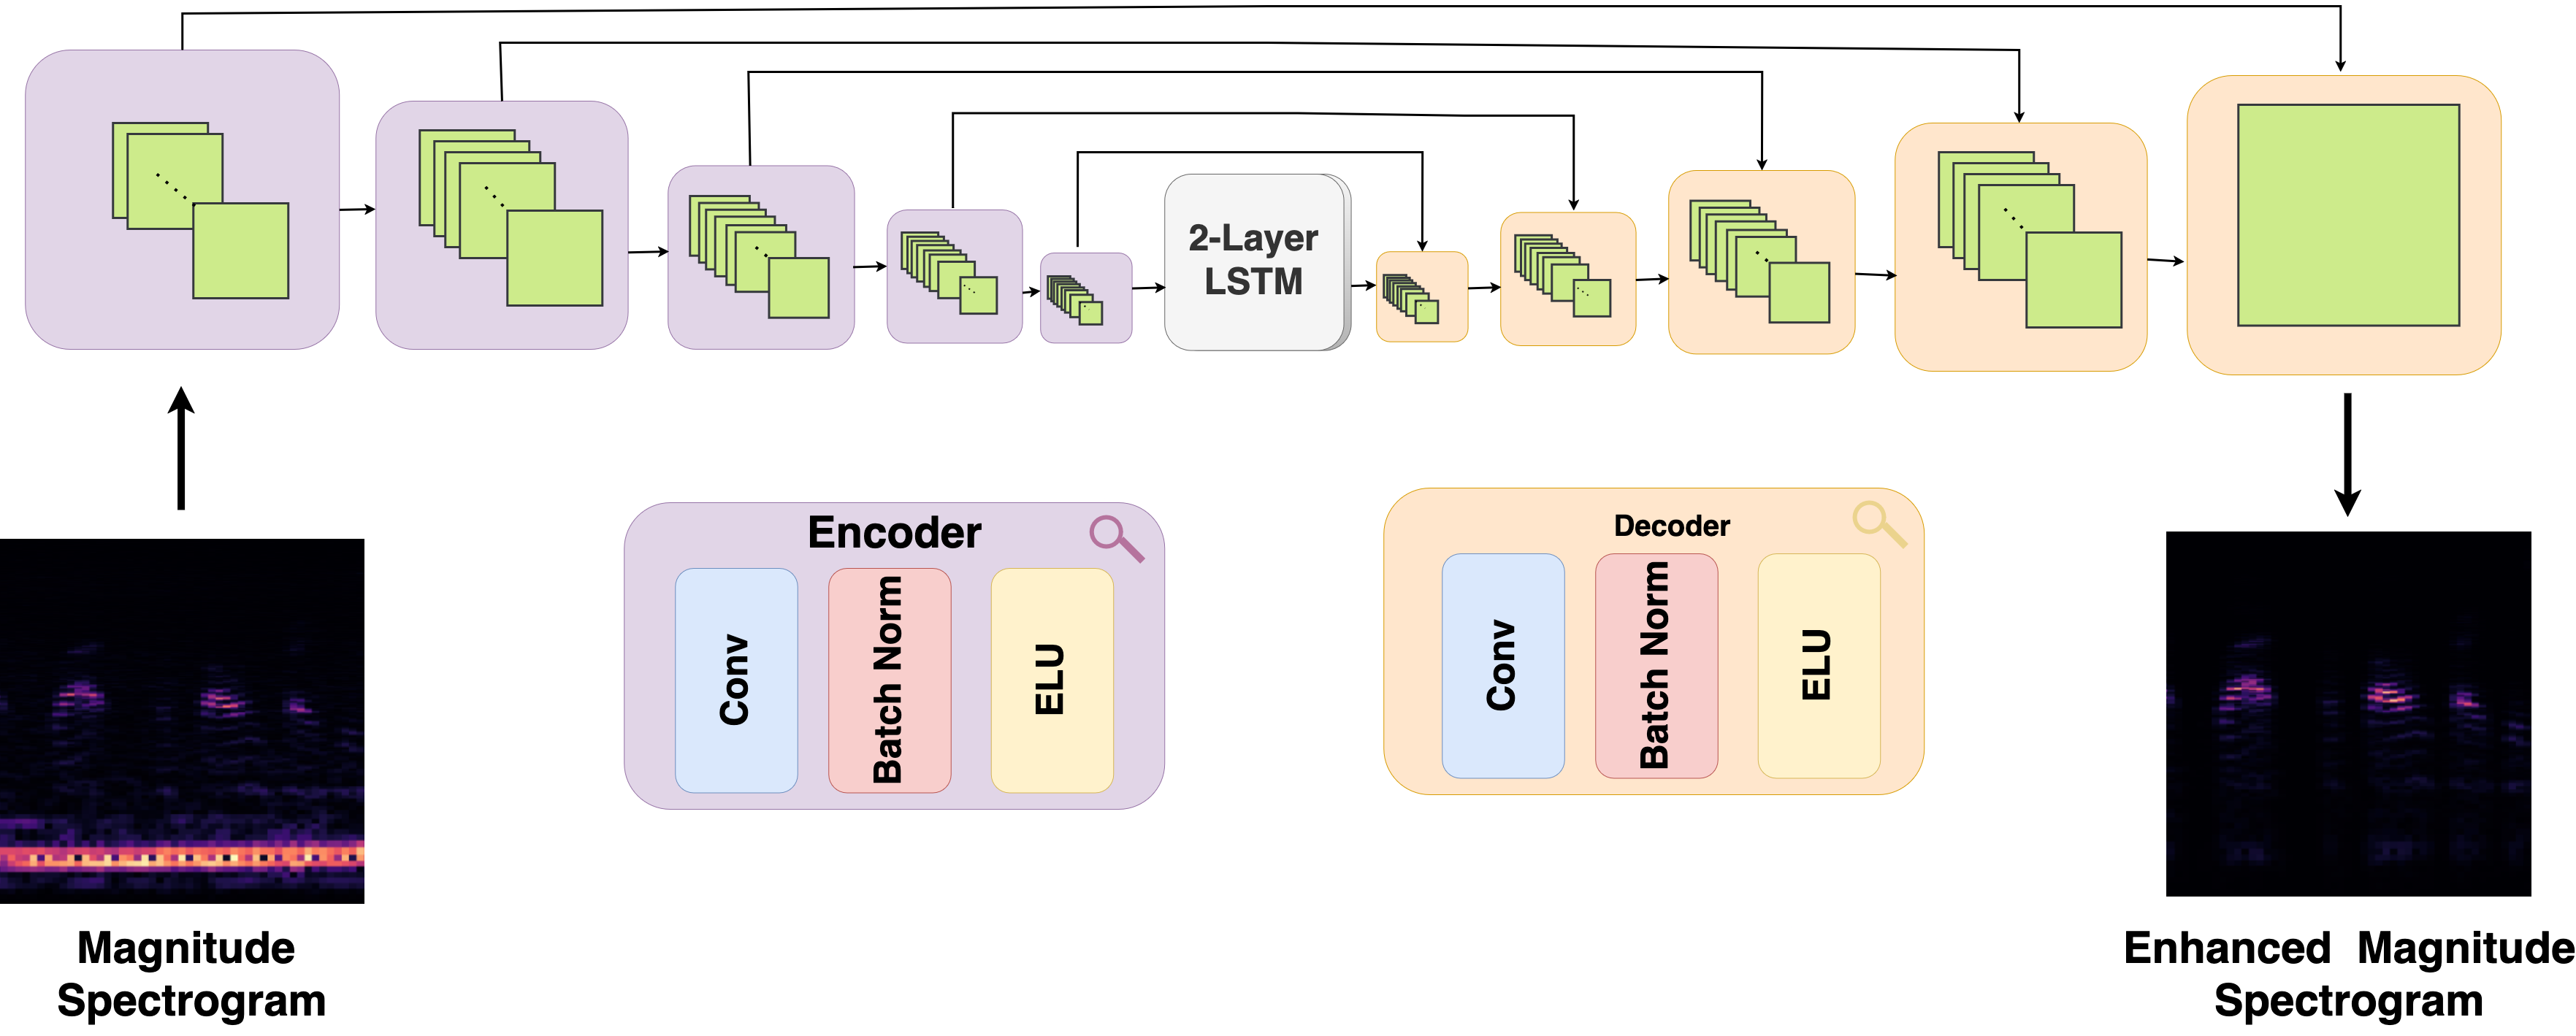
\includegraphics[width=0.95\textwidth]{se-model-diagram-3.png}
   \caption{A diagram of the Convolutional Encoder-Decoder model we will be using for the speech enhancement task.}
   \label{fig:speech-enhancement-model-architecture}
\end{figure}
Mathematically, let a noisy speech signal be represented by \(x \in \mathbb{R}^{T}\) and the corresponding clean speech signal by \(y \in \mathbb{R}^{T}\), where \(T\) denotes the total number of samples.
Speech enhancement is therefore concerned with determining a mapping 
\[
f: \mathbb{R}^{T} \to \mathbb{R}^{T},
\]
which takes a noisy speech signal \(x\) and produces an enhanced version \(f(x)\) that is as close to the clean speech signal \(y\) i.e.
\[
f(x) \approx y.
\]
For this task, $f$ will be implemented by a Convolutional Encoder-Decoder model.
\subsection{Model}
\label{sec:se-model}
As this is more of an exploration of the viability of using a DNN model for speech enhancement 
and the establishment of a baseline which can be used to improve upon in future work, 
we will take into account the work done by \citet{tan18_interspeech} and implement their baseline Convolutional Encoder-Decoder model.
A simplified diagram of the model is shown in Figure \ref{fig:speech-enhancement-model-architecture}.

Instead of using the logmel spectrogram as in the ASA task, we will be using the magnitude spectrogram, 
as did the paper, for consistency. So, the output of the model is a magnitude spectrogram. 

% \begin{table}[h]
%    \centering
%    \begin{tabular}{|c|c|}
%       \hline
%       Layer & Output Size \\
%       \hline
%       Encoder 1 & $16 \times T \times 80$ \\
%       Encoder 2 & $32 \times T \times 39$ \\
%       Encoder 3 & $64 \times T \times 19$ \\
%       Encoder 4 & $128 \times T \times 9$ \\
%       Encoder 5 & $256 \times T \times 4$ \\
%       LSTM & $T \times 1024$ \\
%       Decoder 1 & $128 \times T \times 9$ \\
%       Decoder 2 & $64 \times T \times 19$ \\
%       Decoder 3 & $32 \times T \times 39$ \\
%       Decoder 4 & $16 \times T \times 80$ \\
%       Decoder 5 & $T \times 161$ \\
%       \hline
%    \end{tabular}
%    \caption{The output sizes of the layers in the Convolutional Encoder-Decoder model.}
%    \label{tab:speech-enhancement-output-sizes}
% \end{table}
It will be helpful for this and the forthcoming sections to introduce some notation.
Let $x$ be the input signal (noisy), and let $y$ be the clean speech signal. 
STFT is a function that maps a noisy signal $x$ to a tuple of magnitude and phase spectrograms $(X^{1}, <X^{f})$.
The sizes of the magnitude and phase spectrograms will be $T \times F$ where $T$ is the number of time frames which is 
determined by the length of the signal and the hop size of the STFT. The number of frequency bins $F$ is determined by the 
number of bins specified during the algorithm.
So after applying STFT to $x$, we get $X^{1}$ and $<X^{f}$ and for the clean speech signal $y$, we get $Y^{1}$ and $<Y^{f}$.
The input of the model is $X^{1}$ and the output is $\hat{X}^{1}$. For this to be possible, we need to ensure that the size of the 
magnitude spectrogram is preserved through the model. This is done by fixing the time dimension of the input to the model 
so that no time frames are dropped, but the frequency dimension will change; however, it will return to its original size after the last layer.
So, the stride of the convolutions is set to $(1 \times 2)$ throughout and the kernel size is set to $(2 \times 3)$. 
This has the effect of reducing the frequency dimension by a factor of 2 during encoding and increasing it by a factor of 2 during decoding.
\citet{tan18_interspeech} introduced a Long-Short Term Memory (LSTM) between the encoder and decoder to help with 
the temporal dynamics of speech. So, a 2-layer LSTM with 1024 units is used between the encoder and decoder. This 
requires the need to reshape the output of the LSTM before it is passed into the decoder.
% Table \ref{tab:speech-enhancement-output-sizes} shows the output sizes of the layers in the model assuming 
% that 161 frequency bins are used, so an input of size $T \times 161$ is used.

In terms of what operations are used in the encoder and decoder, after the convolutions (or transposed convolutions in the case of the decoder),
a batch normalisation layer is used. Afterwards, the Exponential Linear Unit (ELU) activation function is used 
as the authors cite that it results in faster convergence and better generalisation. Skip connections 
are also used in the decoder, so the input to each decoder layer is the concatenation of the output of the previous decoder layer 
and the output of the corresponding encoder layer (see Figure \ref{fig:speech-enhancement-model-architecture}).

Since the output of the model is a magnitude spectrogram, we need to convert it back to the time domain. 
The paper by \citet{tan18_interspeech} did not specify which method was used to convert the magnitude spectrogram back to the time domain.
We assume that the authors used the common approach of using inverse STFT (ISTFT) \citep{xu_regression_2015} i.e. the noisy phase spectrogram 
is combined with the predicted magnitude spectrogram to reconstruct the time domain signal $\hat{x}$. In other words,
\[
\hat{x} = \text{ISTFT}(\hat{X}^{1}, <X^{f}).
\]
\subsection{Training}
The training itself will be performed using the Adam optimiser just as in the paper \citep{tan18_interspeech}.
Since the datasets we will be using have clean and noisy speech signals, we can use the noisy speech signal ($x$) as input
and the clean speech signal ($y$) as the ground truth.
Then, the objective of the training is to minimise the loss between the enhanced magnitude spectrogram ($\hat{X}^{1}$) 
and the ground truth magnitude spectrogram ($Y^{1}$).
Therefore, the loss function is defined as follows:
\[
L(X^{1}, Y^{1}) = \frac{1}{T} \sum_{t=1}^{T} (X^{1}_t - Y^{1}_t)^2,
\]
This is the same loss function used in \citet{tan18_interspeech} and is the Mean Squared Error (MSE) loss function.

\subsection{Evaluation}
The performance of the speech enhancement model is evaluated using PESQ and STOI,
serving as proxies for the gold standard of subjective listening tests, which, 
due to the time and cost constraints, are not conducted in this part of the dissertation.
% The evaluation of the speech enhancement model in this part of the dissertation will be 
% done by assessing two artificial metrics. The other approach to evaluation is 
% to use subjective listening tests, which is a gold standard for evaluating speech enhancement models.
% However, as with all gold standard methods, they are time consuming and expensive to conduct. 
% Artificial metrics aim to be a proxy for the gold standard methods. 

Firstly, the Short-Time Objective Intelligibility (STOI) \citep{taal_algorithm_2011} metric will be used to assess the intelligibility of the enhanced speech signal.
It is a function of the noisy speech signal $s_n$ and the degraded speech signal $s_d$ after enhancement.
The STOI metric computes a value in the range \([0, 1]\), which can be interpreted as an approximation of the average percentage of correctly understood words in $s_d$. 
For the sake of brevity, we will not go into the details of the STOI metric, but for the interested reader, we refer them to \citet{taal_algorithm_2011}.

Secondly, the Perceptual Evaluation of Speech Quality (PESQ) \citep{rix_perceptual_2001} metric will be 
used to assess the perceptual quality of the enhanced speech signal. 
This metric is a function of the clean speech signal $s_c$ and the enhanced speech signal $\hat{s}_e$.
PESQ compares $s_c$ and $\hat{s}_e$, yielding a score between 1 (indicating poor quality) and 4.5 (indicating near distortion-free quality). 
As with STOI, the intricate details of the PESQ metric are not discussed here; the reader is encouraged to consult \citet{rix_perceptual_2001} for a complete description.

A valid question to ask is why the model is not trained to directly optimise for both metrics. The primary challenge lies in the fact that both STOI and PESQ are non-differentiable,
which is a problem for gradient-based optimisation frameworks. 
For more details, we discuss this in more detail in section \ref{sec:future-work}.

Feasibility analysis mirrors that of the ASA model, focusing on FLOP(s), parameter count, and theoretical inference time.
\section{Laying the Groundwork for State-Dependent Models}
\begin{figure}[h] \centering
   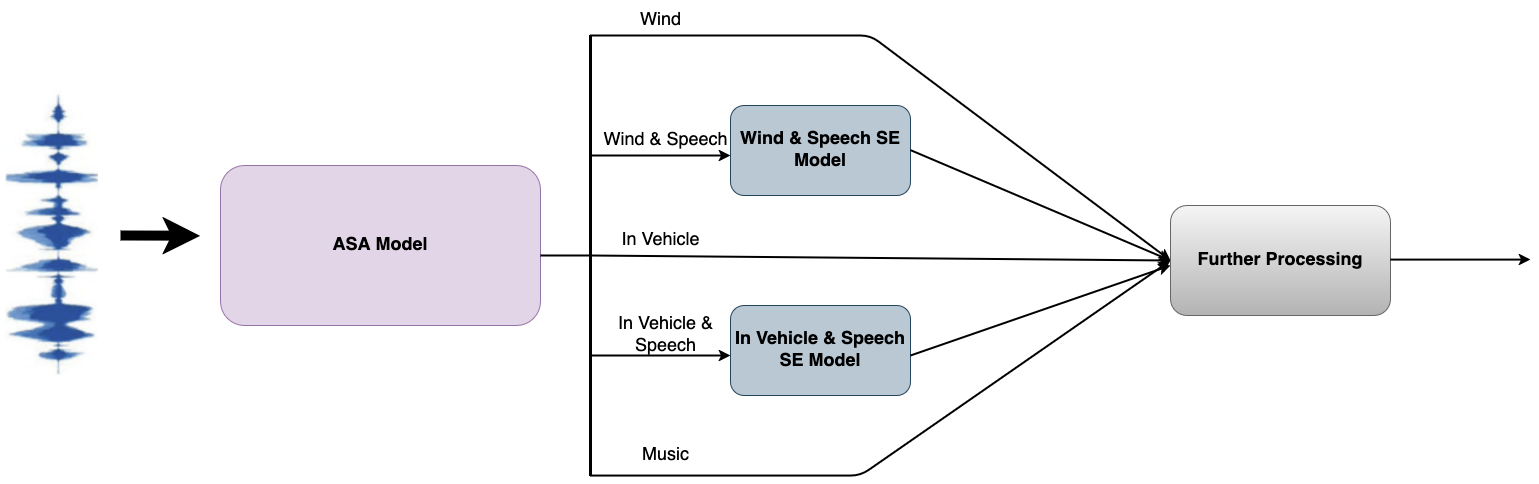
\includegraphics[width=0.9\textwidth]{state-model-diagram.png}
   \caption{The vision we have for the state-dependent model.}
   \label{fig:state-dependent-model}
\end{figure}
In the preceding sections, we have established the groundwork for the two tasks that we will be doing in this part of the dissertation.
The reason we are devising these two tasks in the first place is to set the groundwork for the next part of the dissertation which 
will be focused on the implementation of a state-dependent model. We hypothesise that a feasible state-dependent model can be created 
by chaining the two models together. Figure \ref{fig:state-dependent-model} shows the vision we have for the state-dependent model which we aim to implement fully in the next part of the dissertation.
Mathematically, the state-dependent model can be represented as follows:
\[
f: \mathbb{R}^{T} \to \mathbb{R}^{T},
\]
where \(T\) denotes the total number of samples. 
Then, given a ASA model $g : \mathbb{R}^{T} \to \mathcal{E}$ and a family of SE models $h_{\epsilon} : \mathbb{R}^{T} \to \mathbb{R}^{T}$ for all \(\epsilon \in \mathcal{E}\), 
$f$ can be represented as a piecewise function:
\begin{equation}
   f(x) = 
   \begin{cases} 
      h_{\epsilon}(x) & \text{if } g(x) = \epsilon \\
      x & \text{otherwise}
   \end{cases}
\end{equation}
In other words, the state-dependent model $f$ will apply the SE model $h_{\epsilon}$ to input $x$ if the ASA model $g$ maps $x$ to \(\epsilon\).
For example, if an HA user is situated in an environment characterised as `Wind Turbulence and Speech',
the state-dependent model will invoke the SE model that has been trained on this scenario to enhance the input signal $x$.
The state-dependent model is inspired by the unveiling of the Spheric Clarity DNN model by Phonak \citep{Hasemann2024PhonakSphere} in late 2024
in which if the HA user is faced in a 'Speech in Loud Noise' environment, the input signal $x$ will be passed through their Spheric Clarity DNN model.


\chapter{Experimental Setup}
\label{chap:experimental_setup}
With the methodological foundation laid out in the preceding chapters, we can now outline the hypotheses that we aim to validate.
Although we hinted at some of those hypotheses in the preceding chapters and sections, as a means of clarity, 
we will be outlining the hypotheses again here and in more detail so that the reader can have a comprehensive understanding of both the objectives and the rationale behind the experiments we will be doing.
Once we outline the hypotheses, another section is dedicated towards the datasets that will be used to validate the hypotheses.
Once that is done, the reader will be in a position to analyse the results of the experiments which will be presented in Chapters \ref{chap:asa-experiments} and \ref{chap:se-experiments}.
\section{Hypotheses}
\label{sec:hypotheses}
\begin{enumerate}
   \item \textbf{Replication of ASA Results.} 
   We hypothesise that the results reported by \citet{Huwel2020HearDS} for the ASA task can be replicated using the methodological approach detailed in Section \ref{sec:methodology-asa}.
   Achieving replication is crucial as it brings us a step closer to our vision of creating a state-dependent model in the next part of the dissertation.
   % TODO: Ask Hao if I should rephrase this to reject Huwel's claim that SGD is better than Adam due to weight initialisation issues?
   \item \textbf{Effectiveness of Utterance-Level Data Augmentation}. We hypothesise 
   that if we mix the speech signal with the SNR at an utterance level, we will be able 
   to reduce the training time of the model and have similar performance to that of using 
   every SNR level per epoch. 
   Once again, validating this hypothesis will speed up the development process going forward, 
   since if true, there will be less samples per epoch and thus less training time. 
   \item \textbf{Capability of the Speech Enhancement Model}.
   We hypothesise that the methodological approach detailed in Section \ref{sec:se-model} to 
   create a speech enhancement model will be able to enhance the speech signal by 
   cutting out the background noise. 
   % \item \textbf{Superiority of State-Specific Training}
   % As the end-goal of this dissertation is to create a state-dependent model, we hypothesise that
   % training a model on each environment will result in a better performing model than training on all environments.
   % We believe this could be due to the fact that with a shallower model, the parameters of the models 
   % are less likely to be able to be fitted in such a way that all environments are catered for. 
   \item \textbf{Feasibility of Deployment on Hearing Aid Devices}.
   With the evaluation of the models with respect to the number of FLOP(s) and the size of the models,
   we aim to show that the models we implement are able to be deployed on HA devices. 
   This is a really important hypothesis to validate; otherwise any work 
   we do would not allow us to create a state-dependent model if the dependent models 
   are not able to be deployed on HA devices.
   \item \textbf{Comparative Performance of the Adam Optimiser.}
   It is hypothesised that use of the Adam optimiser will result in a faster convergence with performance comparable to that of using a fixed learning rate Stochastic Gradient Descent (SGD) method, as used in \citet{Huwel2020HearDS}.
   Validating this hypothesis will speed up the development process in the future, 
   and enable uniformity across subsequent experimental iterations. Additionally,
   it will allow us to reach the objective of creating a state-dependent model faster because of the acceleration of the development process.
\end{enumerate}

\section{Datasets}
\label{sec:datasets}

% \begin{table}[h]
%    \centering
%    \begin{tabular}{|c|c|c|c|}
%       \hline
%       Dataset & \rotatebox{90}{Environments} & \rotatebox{90}{No. of Speakers} & \rotatebox{90}{Hours of Data} \\
%       \hline
%    HEAR-DS \citep{Huwel2020HearDS} & 6 & - & 21 hours \\ % TODO: The hours is wrong, find the correct number
%       CHiME 3 (booth dev. set) \citep{barker_third_2015} & - & 4 & 10 hours \\
%       CHiME 6 (train + dev + eval) \citep{barker18_fifth_2018} & - & 48 & 50 hours \\
%       TUT Acoustic Scenes 2016 \citep{mesaros_tut_2016} & 10 & - & 10 hours \\
%       \hline
%    \end{tabular}
%    \caption{Dataset statistics.}
%    \label{tab:dataset-stats}
% \end{table}

\subsection{HEAR-DS}
\label{sec:hear-ds}
\heards is a dataset created by \citet{Huwel2020HearDS} that is specially designed for Hearing Aid (HA) research. 
It consists of recordings captured on a dummy head equipped with three microphones per side: one In-The-Canal (ITC) [in the ear] and two Behind-The-Ear (BTE) microphones (front and rear).
Each sample is recorded in either the left or right channel and decomposed into its respective microphone channels (BTE\_front, BTE\_rear, ITC), available in 48kHz/32bit format.
In the paper, the researchers used only the ITC samples, so for the scope of this project, we will use only the ITC samples as well. 
Because the researchers were based in Germany, any recordings that they took were situated in Germany.
The dataset provides 7 environments:
\begin{itemize}
   \item \textbf{Cocktail Party} - Covers situations such as multiple speakers in a noisy environment or 'babble' noise. The paper mentions that this was mimicked by recording them in a university cafeteria or at a senior citizens' meeting.
   \item \textbf{Wind Turbulence} - Concerns the sound that is produced when the wind passes through a microphone.
   \item \textbf{In-Traffic} - Samples where traffic noise is dominant such as bus stations or sidewalks. The researchers controlled for this environment not to be similar to the \textit{Wind Turbulence} environment by choosing 'calm' days for the recordings.
   \item \textbf{In-Vehicle} - The sounds produced when sitting inside a car. The researchers controlled for this environment to not be similar to the \textit{In-Traffic} or \textit{Wind Turbulence} environments by ensuring the windows were closed. 
   \item \textbf{Quiet Indoors} - Mimic noises produced in a typical household such as washing dishes, clock ticking, etc. The researchers controlled for variability by recording the samples in several flats (rural, city centre, etc).
   \item \textbf{Reveberant} - Samples in highly reverberant environments such as a railway station hall, staircases or a church. 
   \item \textbf{Music} - The data is actually taken from the GTZAN dataset \cite{tzanetakis_musical_2002} and is used to test the model's ability to classify music.
\end{itemize}
Furthermore, the researchers artificially created a new environment, \textit{Interferring Speakers}, which are samples that contain speech from multiple speakers. 
This is done by taking speech samples from the
\chime{5} dataset \cite{barker18_fifth_2018}. This environment is supposed to mimic the 
typical conversational speech that occurs in a real-world scenario. We however, decided to use the \chime{6} dataset which 
supersedes the \chime{5} dataset \cite{barker18_fifth_2018} by correcting the alignment of audio channels and the researchers 
recommend the use of the \chime{6} dataset instead of \chime{5} for any new research so we will use that instead. This could 
be an important factor as the methodology of creating the \textit{Interferring Speakers} environment is by finding 10s 
segments of speech that contain multiple speakers, so if the alignment of audio channels is not correct, the recordings 
may have a delay between the left and right channels, which could potentially affect the results of the paper. 
In any case, the way this environment was created is unclear from the paper, but we do the following approach to create the environment:
\begin{enumerate}
   \item The code processes \chime{6} sessions to find 10-second segments that contain overlapping speech from multiple speakers.
   \item For each segment, it extracts audio from the reference speaker's microphone and saves both left and right channels.
\end{enumerate}

To prevent the model from overfitting and increase the diversity of the data, the researchers provided multiple REC-SITs (Recording Situations) for each environment.
In the case of the \textit{Music} environment, each REC-SIT represents a different genre of music. This has some potential to cause problems, 
and we discuss this in more detail once we aim to reproduce the results of the paper (Chapter \ref{chap:asa-experiments}).  % TODO: Explain the issue later
As for the artificially created \textit{Interferring Speakers} environment, it is unclear how they define REC-SITs for this environment. 
What we did was to extract the session ID from the \chime{6} dataset and use that as the REC-SIT, which 
gives us a total of 16 REC-SITs for this environment.

At the REC-SIT level, the raw dataset comprises multiple cuts, each cut not necessarily of uniform duration.
In accordance with the methodology of the original study, each cut was segmented into 10s snippets.
Table \ref{tab:hear-ds-stats} presents the distribution of samples in the various environments after segmentation.
In general, our statistics are largely consistent with the original report, though with minor discrepancies in the \textit{Interferring Speakers} and \textit{Cocktail Party} environments.
Specifically, our version of the \textit{Interferring Speakers} environment comprises 1,364 samples compared to the 1,481 reported originally, a difference that may be attributable to the alignment issues mentioned above in the \chime{5} dataset.
Similarly, the \textit{Cocktail Party} environment contains 716 samples in our dataset as opposed to 667 in the original report — a discrepancy that could potentially result from a typographical error in the original document. 

\begin{table}[h]
   \centering
   \begin{tabular}{|c|c|}
      \hline
      Environment & Total No of Samples \\
      \hline
      Cocktail Party & 716 \\
      Wind Turbulence & 1364 \\
      In-Traffic & 1000 \\ 
      In-Vehicle & 1094 \\
      Quiet Indoors & 951 \\ 
      Reverberant & 1007 \\ 
      Music & 2991 \\
      Interferring Speakers & 1364 \\
      \hline
   \end{tabular}
   \caption{\heards dataset statistics after cutting each environment's cuts into 10s snippets.}
   \label{tab:hear-ds-stats}
\end{table}

As noted in the Introduction, the model can be made to act as a Voice Activity Detector (VAD) by incorporating environments with and without speech.
The raw dataset however, only contains samples without speech, so we will be following the paper's approach to create the mixed environments.
Although recording environments with and without speech was something the researchers did consider, the researchers prioritised full control over the SNR during the speech-background mixing process.
The speech mixing that the paper described is something we 
will have to deviate from, at least for this part of the dissertation.
Firstly, while the paper uses a head-related transfer function (HRTF) to mix the speech signal with the background noise,
we will not be using it due to time constraints and the scarcity of readily usable libraries.
Furthermore, the paper uses the \chime{2} dataset \citep{vincent_second_2013} to mix the speech signal with background noise.
However, this is not a dataset we were able to get in time for this part 
of the dissertation, so instead we will be using the \chime{3} dataset \citep{barker_third_2015} to mix the speech signal with background noise.
We discuss this limitation in more detail in Section \ref{sec:future-work}.
Otherwise, the speech mixing itself is done in a similar manner to the paper.
Firstly, the paper mentions that they ensure that each mixed 10-second snippet contains at least 7.5 seconds of speech.
The speakers are picked at random, and for better generalisation, the speaker is also randomly 
picked at each SNR level, so the same snippet of background noise is very likely 
to have different speech signals mixed with it at different SNR levels.
Given that we will be training and testing the model, the need for a training and test set is imperative. 
% It was not clear how the researchers split the speakers for the mixed environments, so we will be splitting the speakers into two groups—one for training and one for testing.
% Table \ref{tab:dataset-stats} shows that the CHiME 3 dataset contains 4 speakers, and conveniently enough an equal split of gender,
% thus we ensured for generalisability that each set contained a male and female speaker. 

\subsection{CHiME-3}
 As mentioned earlier, we opted for using the \chime{3} dataset to mix the speech signal with the background noise. 
\chime{3} is a dataset published in 2015 for ASR tasks and was dedicated to improving the performance of mobile devices 
in noisy, everyday environments. The vocabulary of the speech samples is taken from a subset of the Wall Street Journal (WSJ0) corpus \citep{wsj0}.
For brevity, we will not go into the details of the environments, as we 
are only interested in the speech samples. 
We use the development set for the mixing process,
and since this dataset contains noisy samples, we will only use clean speech samples 
which is the BOOTH environment.

It contains 10 hours of data from 4 speakers. This could be a problem in both tasks (ASA and Speech Enhancements); in the former
we could be overfitting to the data due to the Pigeon-hole principle i.e. we have much more background samples than speech samples, 
and in the latter, the enhancement model may not generalise well to real-world scenarios due to the small size of the dataset. 

% A better approach would of perhaps been to to use the ORG environment which is a clean set of speech samples from the WSJ0 corpus 
% which has 15.15 hours of data from 83 speakers \cite{barker_third_2015}.
% Nevertheless, we will continue with the paper's approach to set up a baseline. The data was already in 16KHz so we did not need to 
% resample it. 

\subsection{CHiME-5/CHiME-6}
In the paper by \citet{Huwel2020HearDS}, the authors used the \chime{5} dataset to create the \textit{Interferring Speakers} environment for the \heards dataset.
However, since the \chime{6} dataset supersedes \chime{5} with improved audio channel alignment, we opted to use \chime{6} for our implementation.
\chime{6} (and \chime{5}) was a dataset created for the Speech Seperation and Recognition Challenge in 2020. It 
focuses on conversational speech in everyday home environments, and particular emphasis was placed on 
eliciting a 'dinner party' scenario i.e. a mixture of speech from multiple speakers. It was not 
clear from the paper what sets were used for the creation of the \textit{Interferring Speakers} environment 
however, they did provide a table of number of samples in each environment. From the table, we 
were able to deduce that they must have used the training, development and evaluation sets for the creation of the \textit{Interferring Speakers} environment.
As mentioned in Section \ref{sec:hear-ds}, there is a slight discrepancy in the number of samples in the \textit{Interferring Speakers} environment, 
that we obtained and the number of samples reported in the paper. We hypothesise that this is due to the alignment issues aforementioned in the \chime{5} dataset.
The dataset itself contains 50 hours of data from 48 speakers.

\subsection{TUT Acoustic Scenes 2016}
As mentioned in the previous chapter, we were getting better results than the baseline model in the paper by \citet{Huwel2020HearDS} 
so as a means of validation, I decided to use the TUT Acoustic Scenes 2016 dataset \citep{mesaros_tut_2016} to test the performance of the model.
In particular, we will be comparing the results by \citet{schindler_multi-temporal_2018}. The paper presents a multi-temporal approach to ASA, and 
the authors have used the development set of the TUT Acoustic Scenes 2016 dataset for their experiments. It is worth stressing 
that this dataset contains background noise only and the paper does not evaluate it with speech, so when we use it to validate 
the model, we will maintain the same approach as in the paper.
The TUT Acoustic Scenes 2016 dataset contains 10 hours of data from 10 environments.
For brevity, we skip the details of the environments, and focus on the results we obtained, though consult the paper for more details.

\subsection{VOICEBANK + DEMAND}
Just as with the motivation of using TUT Acoustic Scenes 2016 for validating the model's performance in ASA,
we will be doing model validation of speech enhancement. 
For this, we have chosen a dataset collated here at Edinburgh University by \citet{valentini-botinhao_speech_2016}. 
As the name of the dataset suggests, it is a culmination of the VOICEBANK \citep{voicebank} and DEMAND \citep{demand} datasets, 
where the former contains clean speech samples and the latter contains noisy background samples.
We have chosen in particular to use the paper by \citet{kim_specmix_2021} to validate the model's performance.
The reason is two-fold. IN addition to the paper also using the \vbd dataset,
there is potential for future work to employ the data augmentation technique `SpecMix' proposed.
\chapter{Acoustic Scene Analysis Experiments}
\label{chap:asa-experiments}
\section{Data Preparation}
\label{sec:data-preparation}
As one of our hypotheses is to replicate the results of the paper by \citet{Huwel2020HearDS}, 
we will be aiming to follow the same approach to prepare the data for the ASA task.
We outline the approach in the following.

To avoid overfitting, we will divide the data into a training and test set just as the paper did.
The samples identified by REC-SITs allow us to do this easily. The paper mentions that they randomly 
assigned each REC-SIT to either the training or test set. It is unclear if 
that means that theoretically there could be more than one REC-SIT in the test set, which 
leads to a split that is more skewed towards the test set. We instead opted to randomly pick 
one REC-SIT for the test set and the rest for the training set; this gives a more 
skewed split towards the training set, which is more common in the literature.
We will be doing 5 experiments, unlike the paper's 50 due to time constraints. So 
we have 5 different splits of the data for the training and test set that we will be using 
for all experiments (including SE).

Secondly, it is unclear if the paper used any data augmentation techniques, and we 
hypothesised that they perhaps did due to the high epoch count of 240 - to perhaps 
account for needing to train the model for a longer time to converge. However,
since of our hypotheses is to validate the effectiveness of utterance-level data, 
augmentation which we investigate in \ref{sec:data-augmentation}, we will 
not use any augmentation in the baseline for methodological consistency. This means that each mixed speech sample will have 15
SNR levels that will be trained and tested for [-21, -18, -15, -12, -9, -6, -3, 0, 3, 6, 9, 12, 15, 18, 21].

Thirdly, as the CNN model excepts a logmel spectrogram as input, we need to convert the waveform
to a logmel spectrogram. The paper decides to only use the ITC channel for the input, so we 
will follow suit.
For the feature transformation \(\phi\), we will be using the same approach as the paper. Namely, 
\begin{equation}
\phi(x_l, x_r) = \frac{20\log_{10}\left(M X_{L}^{1} \right) + 20\log_{10}\left(M X_{R}^{1}\right)}{2}
\label{eq:logmel}
\end{equation}
which is the arithmetic mean of the logmel spectrogram of the left and right channels of the ITC microphone.
$M$ is the mel filter bank matrix, and $X_{L}^{1}$ and $X_{R}^{1}$ are
the resulting magnitude spectrograms after doing STFT on the left and right channels of the ITC microphone respectively ($x_l$ and $x_r$).

In terms of the parameters of the STFT, we will be using a FFT window length of 1024 samples with a window length of 40ms and a hop length of 20ms. It is 
unclear which window function was used, but we will be using a Hann window as is standard in the literature.
After computing the STFT, we then perform a mel filter bank transformation to obtain the mel filter bank coefficients. 
Of which we extract 40 mel bands. For a 10s snippet of audio, the resulting tensor is of shape $40 \times 500$.
To control for the training time not being affected by the IO 
calls to retrieve the samples and then computing the logmel spectrograms,
we precompute the spectrograms before training.

As mentioned in the methodology section, we will be training 3 models 
(net-8, net-20 and net-32) so in the following experiments, we will 
be training these models with the configurations outlined below.

All of the experiments were performed with PyTorch on a batch size of 32.

\section{Baseline: Fixed Learning Rate SGD Approach}
\begin{figure}[h]
   \centering
   \begin{subfigure}[b]{0.45\textwidth}
      \centering
      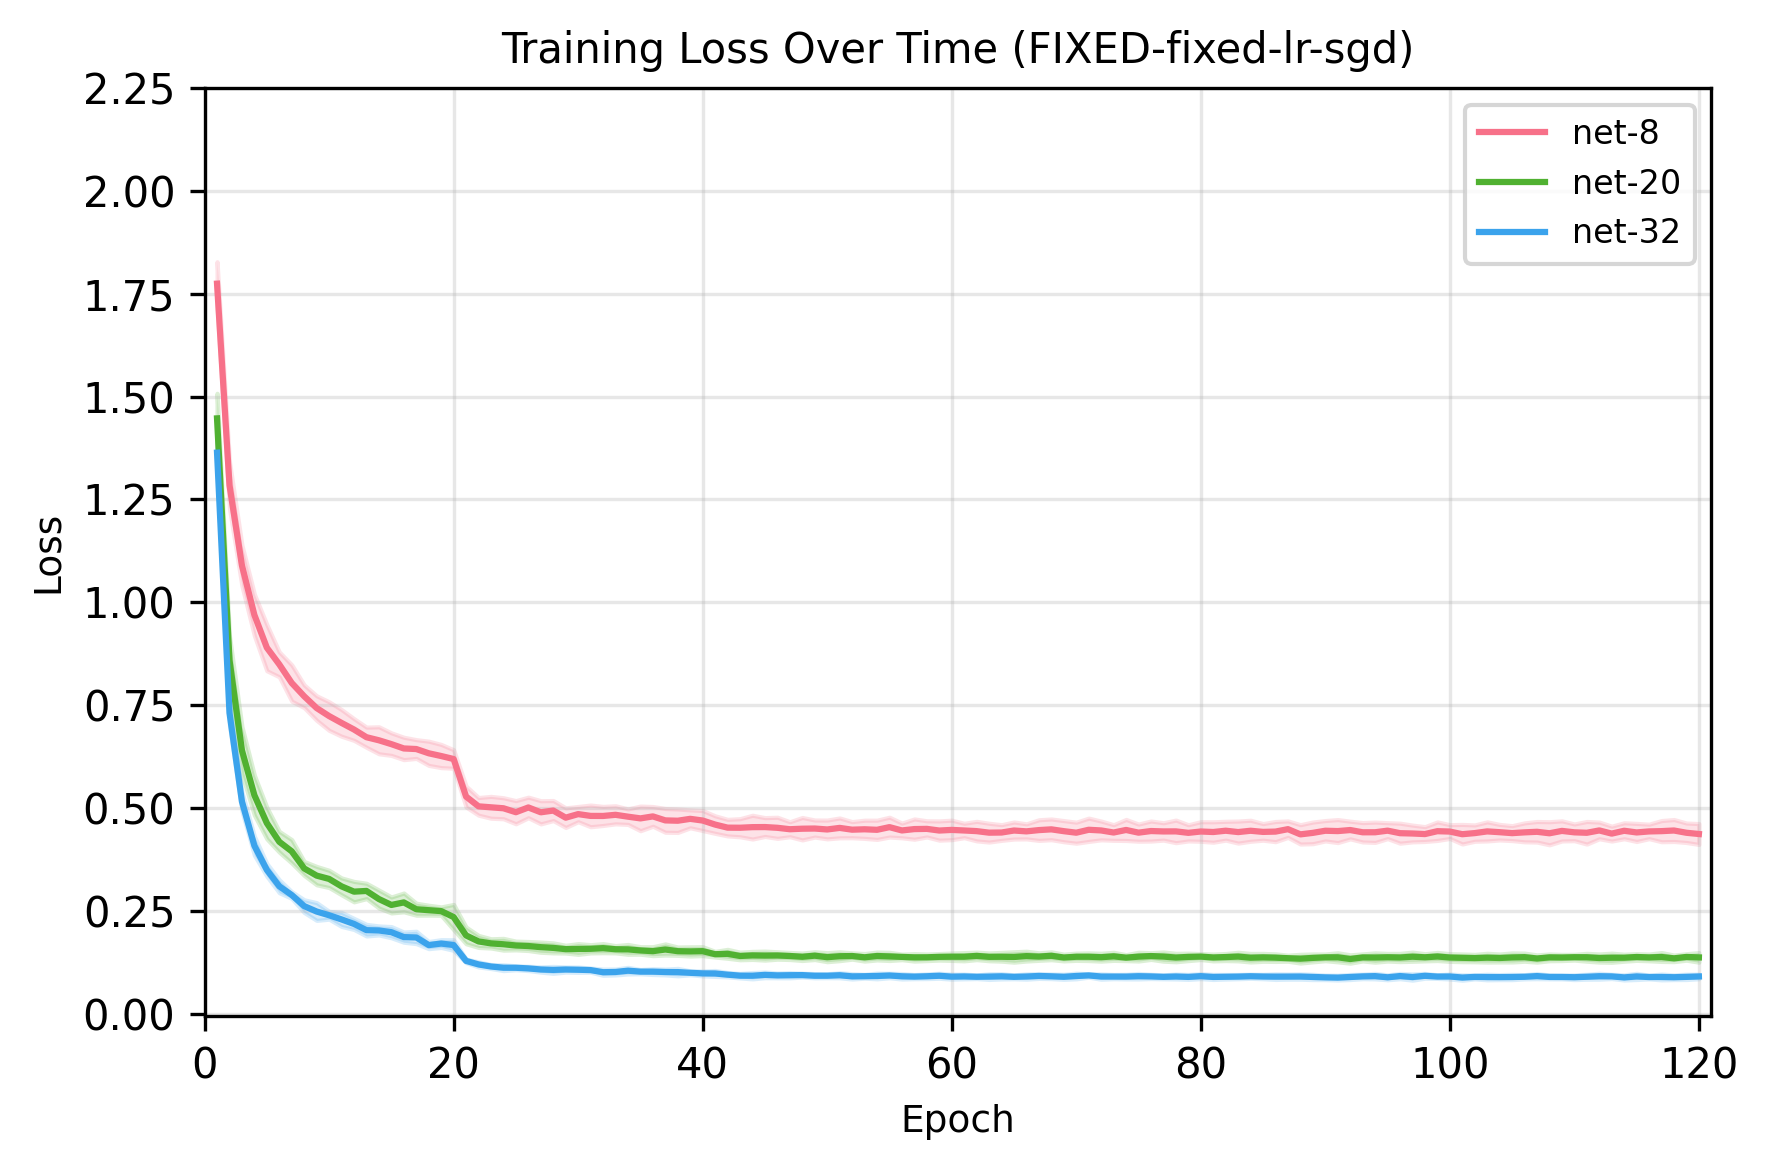
\includegraphics[width=\textwidth]{FIXED-fixed-lr-sgd_training_losses.png}  
      \caption{}
      \label{fig:fixed-lr-sgd-losses}
   \end{subfigure}
   \begin{subfigure}[b]{0.45\textwidth}
      \centering
      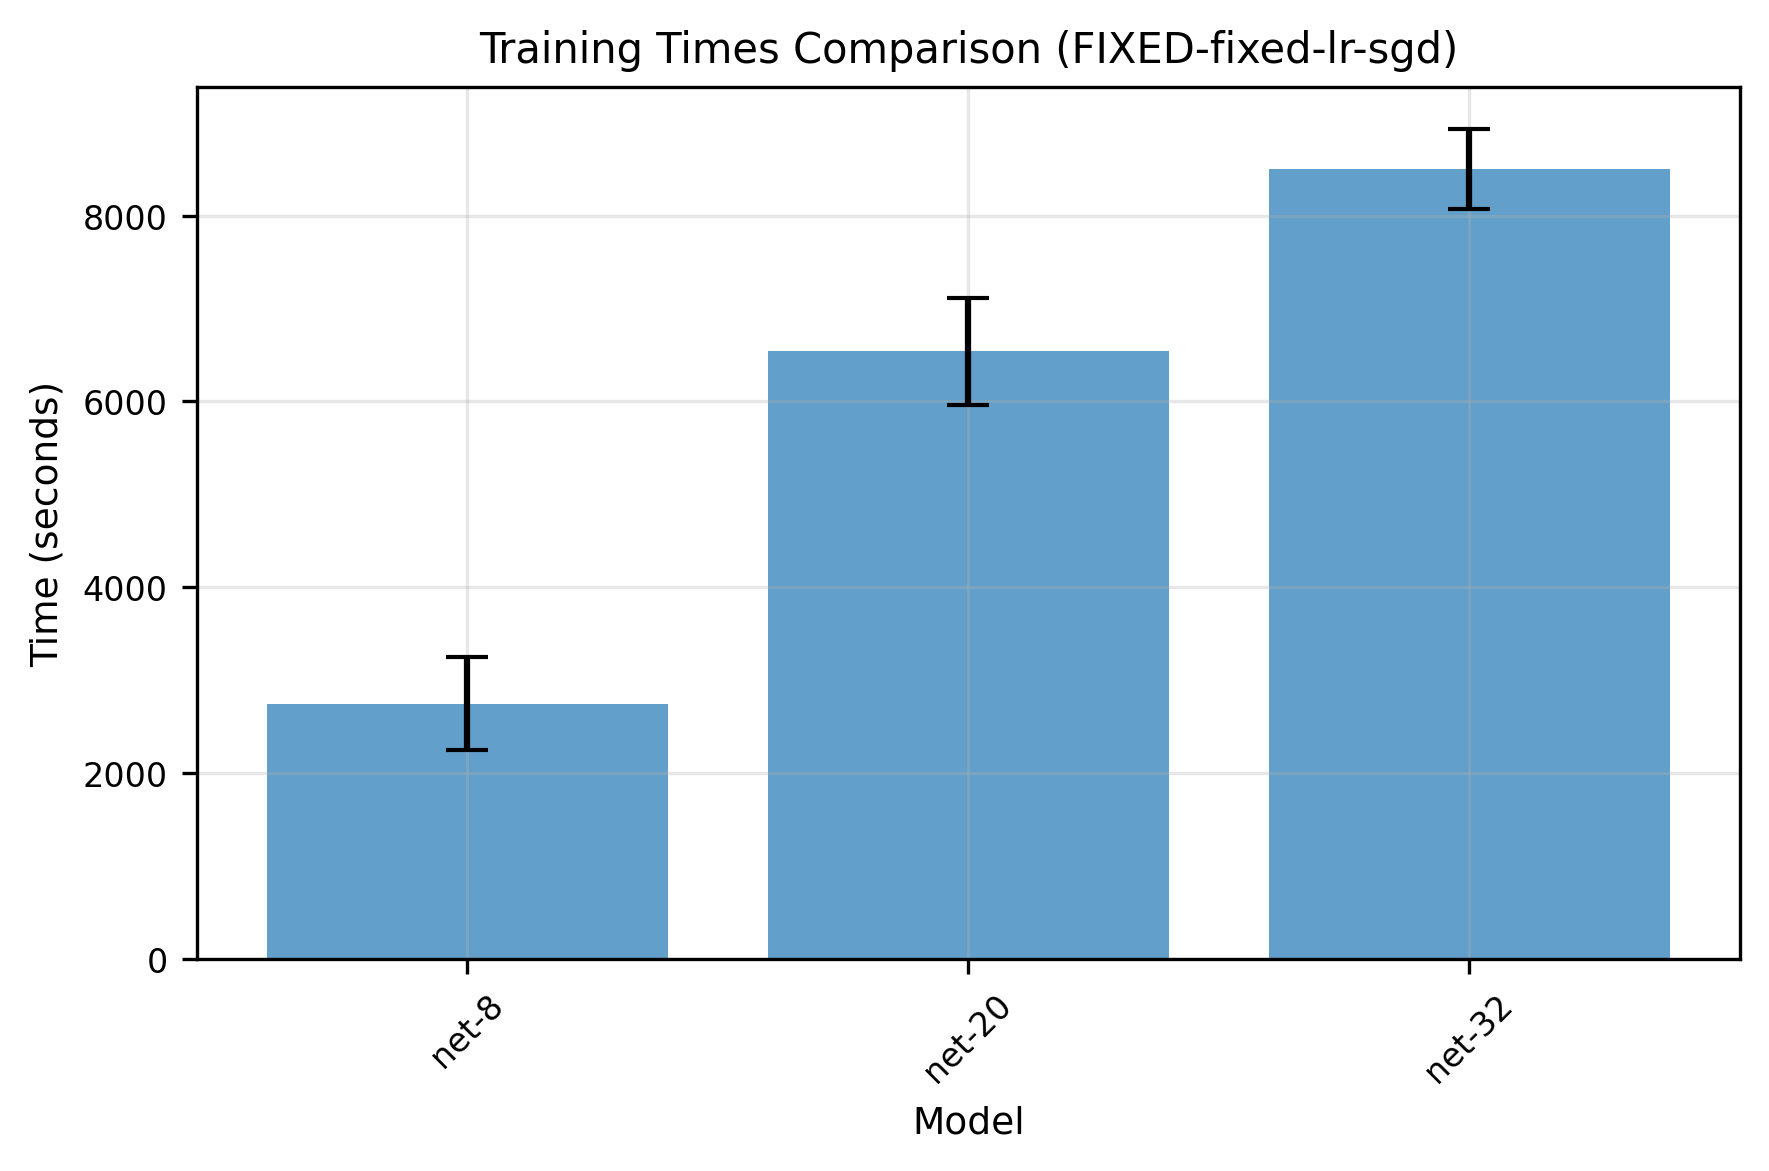
\includegraphics[width=\textwidth]{FIXED-fixed-lr-sgd_training_times.png}
      \caption{}
      \label{fig:fixed-lr-sgd-times}
   \end{subfigure}
   \caption{The training curve (\subref{fig:fixed-lr-sgd-losses}) and training times (\subref{fig:fixed-lr-sgd-times}) of the net-8, net-20 and net-32 models when using the fixed learning rate SGD approach.}
   \label{fig:training-curves}
\end{figure}
With the data preparation out of the way, we can now move on to the experiments.
For the baseline, we will follow the approach of the paper with using the following 
learning rates: [0.05, 0.01, 0.001, 0.0005, 0.0002, 0.0001].
The learning rate in the paper is changed every 40 epochs, however, as that means doing 
240 epochs, we decided to do 120 epochs instead and so change the learning rate every 20 epochs.
As can be seen in Figure \ref{fig:fixed-lr-sgd-losses}, the model already converges by 120 epochs,
indicating that the additional epochs in the original paper were not necessary. 
Moreover, the minimal variability observed in the training curve in the 5 experiments 
raises questions about why the paper by \citet{Huwel2020HearDS} did 50 experiments. Unfortunately,
the lack of access to the original paper's training curves means that we cannot investigate this further. 

\begin{figure}[h]
   \centering
   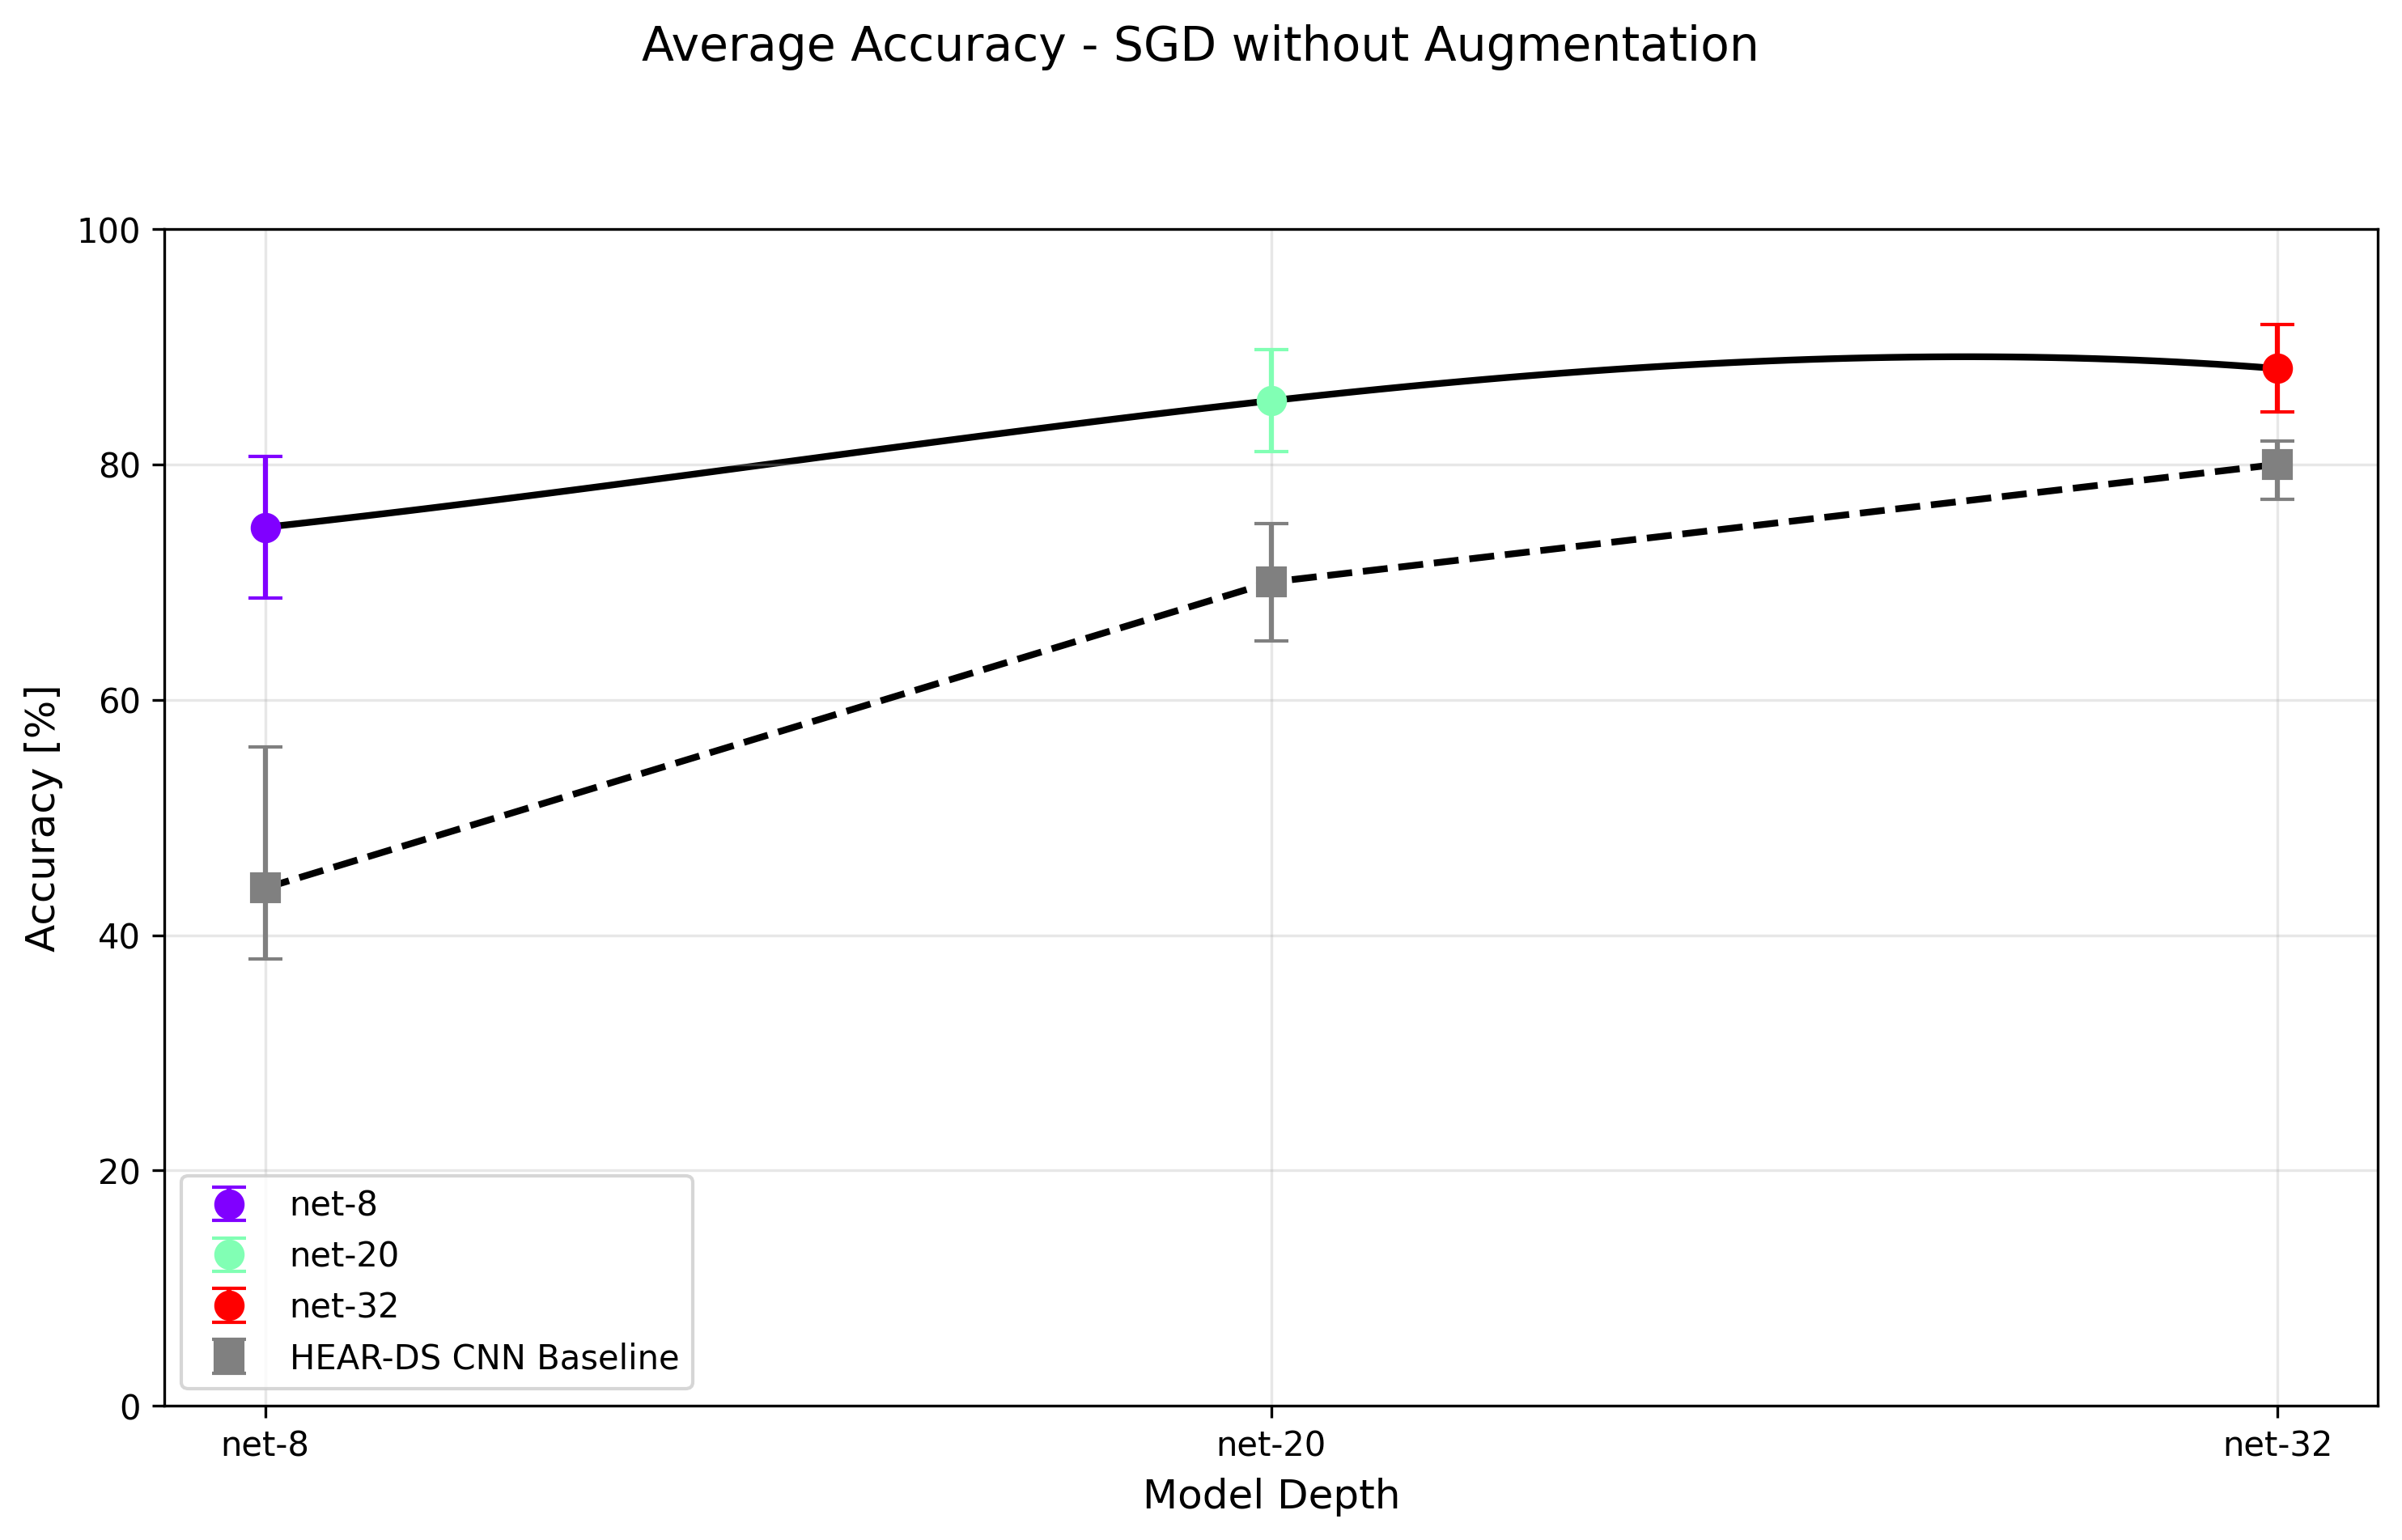
\includegraphics[width=0.8\textwidth]{average_accuracies_sgd_no_aug.png}
   \caption{The average accuracies fitted with linear regression of the net-8, net-20 and net-32 models when using the fixed learning rate SGD approach.
   Also plotted are the extrapolated results from \citet{Huwel2020HearDS} for the three models.
   }
   \label{fig:fixed-lr-sgd-accuracies}
\end{figure}

Figure \ref{fig:fixed-lr-sgd-accuracies} demonstrates the model's performance on the test set after training for 120 epochs 
with the results of the paper by \citet{Huwel2020HearDS} also plotted. It is clear 
that with using a more powerful model, we are able to achieve a higher accuracy 
as seen by the positive slope of the increasing accuracy with model size.
Our accuracies are much higher than the paper's, and we are not getting a gradual 
increase in accuracy as they are. For further investigation, we 
compare our classwise accuracies of the net-20 model against theirs in Figure 
\ref{fig:fixed-lr-sgd-classwise-accuracies}. It is encouraging 
that the overall trends between our results and the paper's are similar. 
Namely, it seems to be struggling a lot more with the Cocktail Party, Reverberant 
Environment and the Speech In Wind Turbulence environments.
It is also interesting that the paper's results have a lot more variance in the classwise accuracies 
just as we have seen in the training curves. We can only hypothesise 
that this is due to the different speech dataset used (CHiME 3 instead of CHiME 2) 
and perhaps the inclusion of the HRTFs during the speech mixing process. We leave 
this for future work to investigate.

\begin{figure}[h]
   \centering
   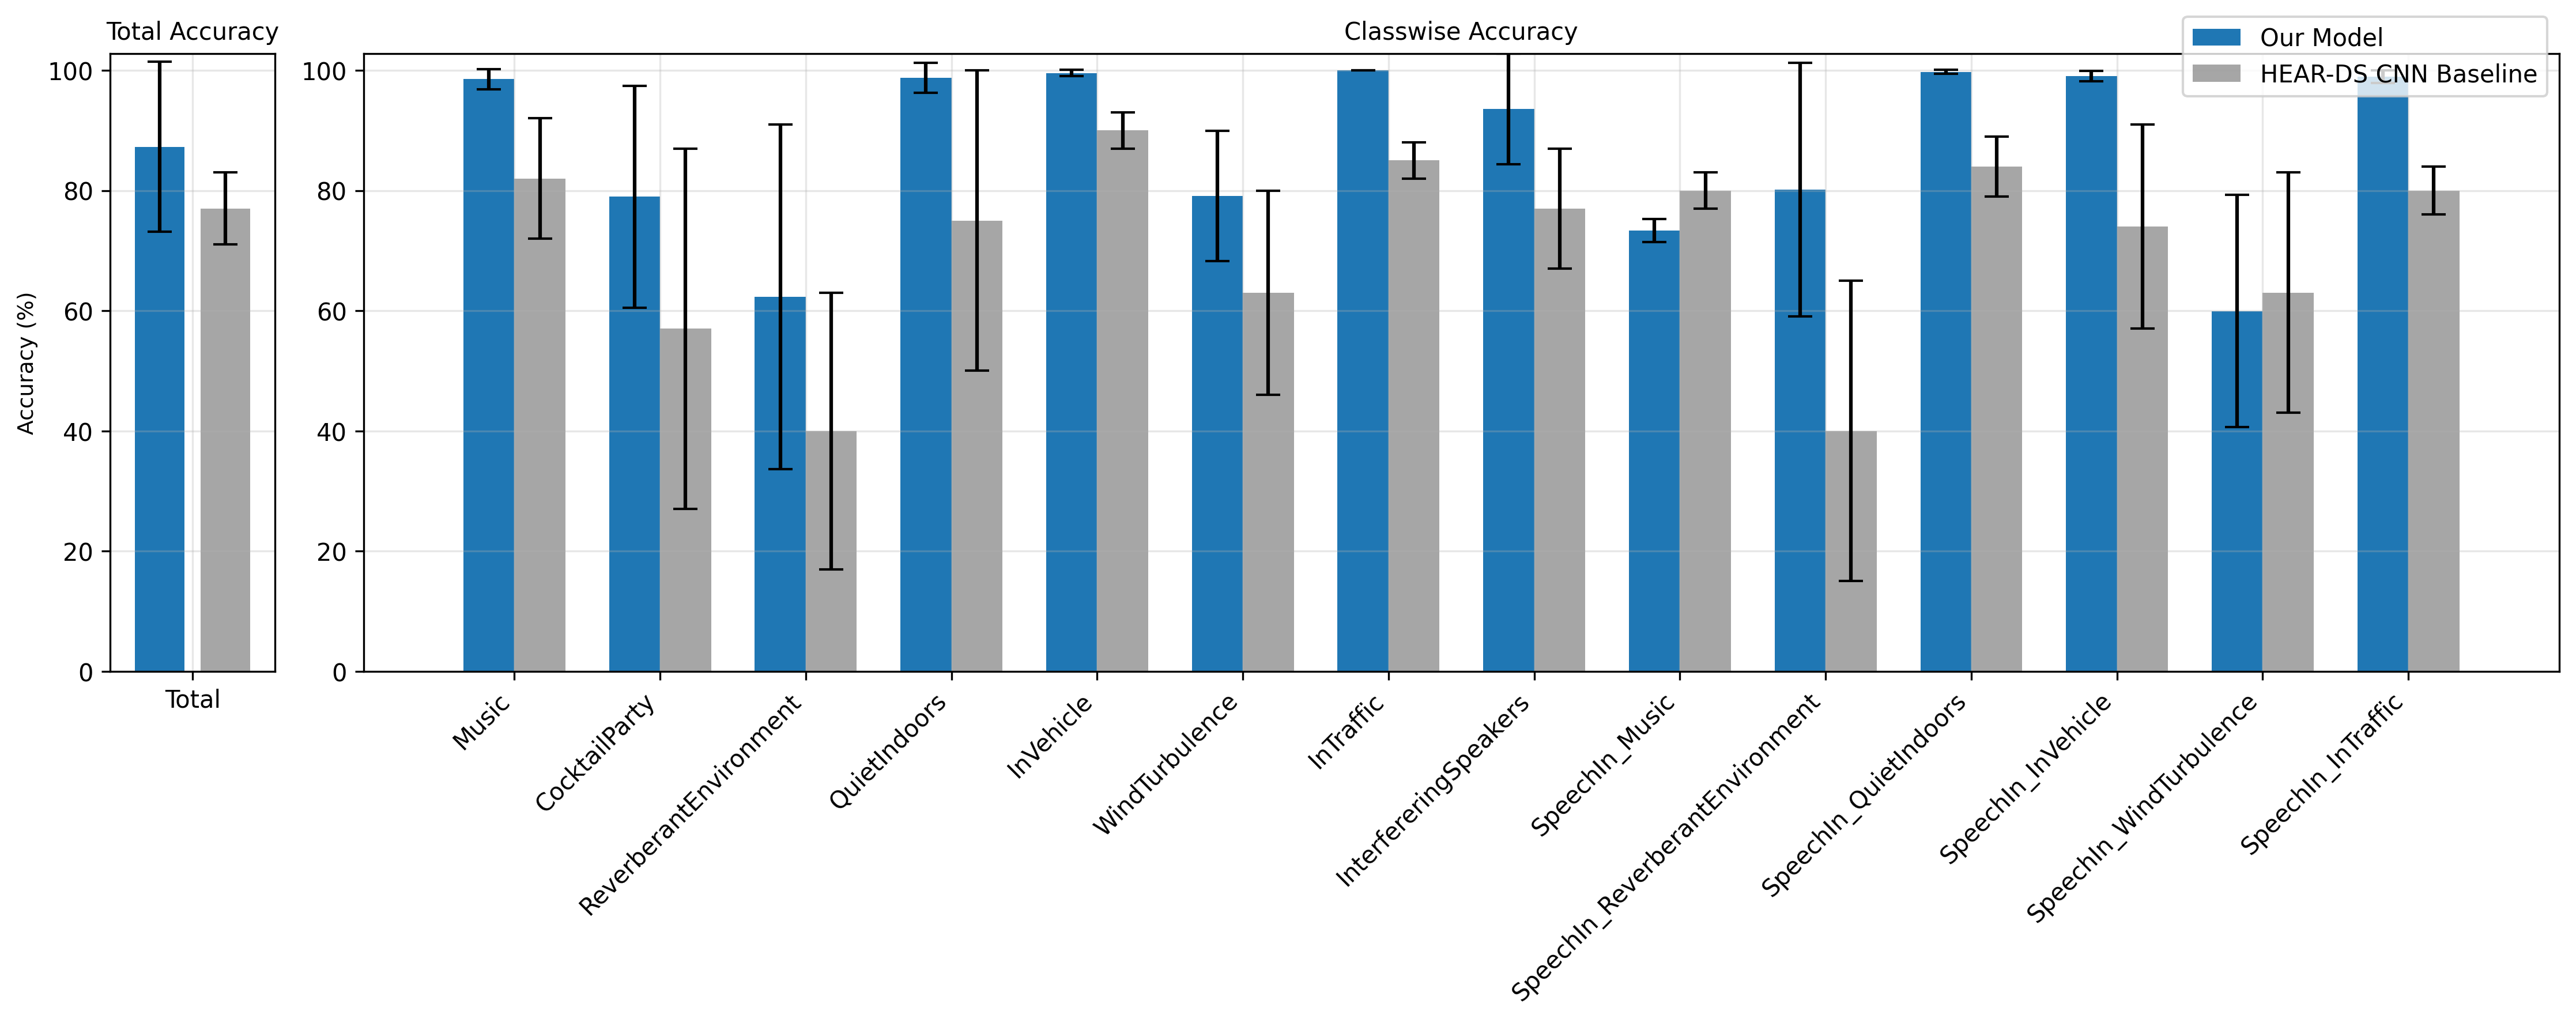
\includegraphics[width=0.8\textwidth]{net-20/FIXED-fixed-lr-sgd/classwise_accuracies.png}
   \caption{The classwise accuracies of the net-20 model when using the fixed learning rate SGD approach.
   Also plotted are the extrapolated classwise accuracies from Figure 3 of \citet{Huwel2020HearDS} for comparison.}
   \label{fig:fixed-lr-sgd-classwise-accuracies}
\end{figure}   

As discussed in the previous chapter, in each of the classification experiments, we felt like reporting just the overall 
accuracies was not enough to get a holistic view of the model's performance. 
So we wanted to investigate the model's performance on specific SNRs and also by reporting the precision, recall and F1 scores to
see if the model is performing well for all classes. 

For the sake of brevity, our investigation focuses on the two extremes of the SNRs,
(-21dB, 21dB) and seen through the lens of two models: net-8 and net-32.
The lowest SNR (-21) gives an indication of
how well the model is able to reliably detect the presence of speech 
even when background noise is barely discernible, although it 
may struggle to differentiate between various environments.
The highest SNR (21dB) evaluates the model's
ability to identify the correct environment in situations with significant background noise, albeit possibly at the expense of accurately detecting the presence of speech.
The selection of net-8 and net-32 allows us to assess whether increased model complexity enhances the model's sensitivity to these nuances, particularly in terms of capturing subtle differences in performance across varying SNR conditions.

\begin{figure}[h]
   \centering
   \begin{subfigure}[b]{0.48\textwidth}
      \centering
      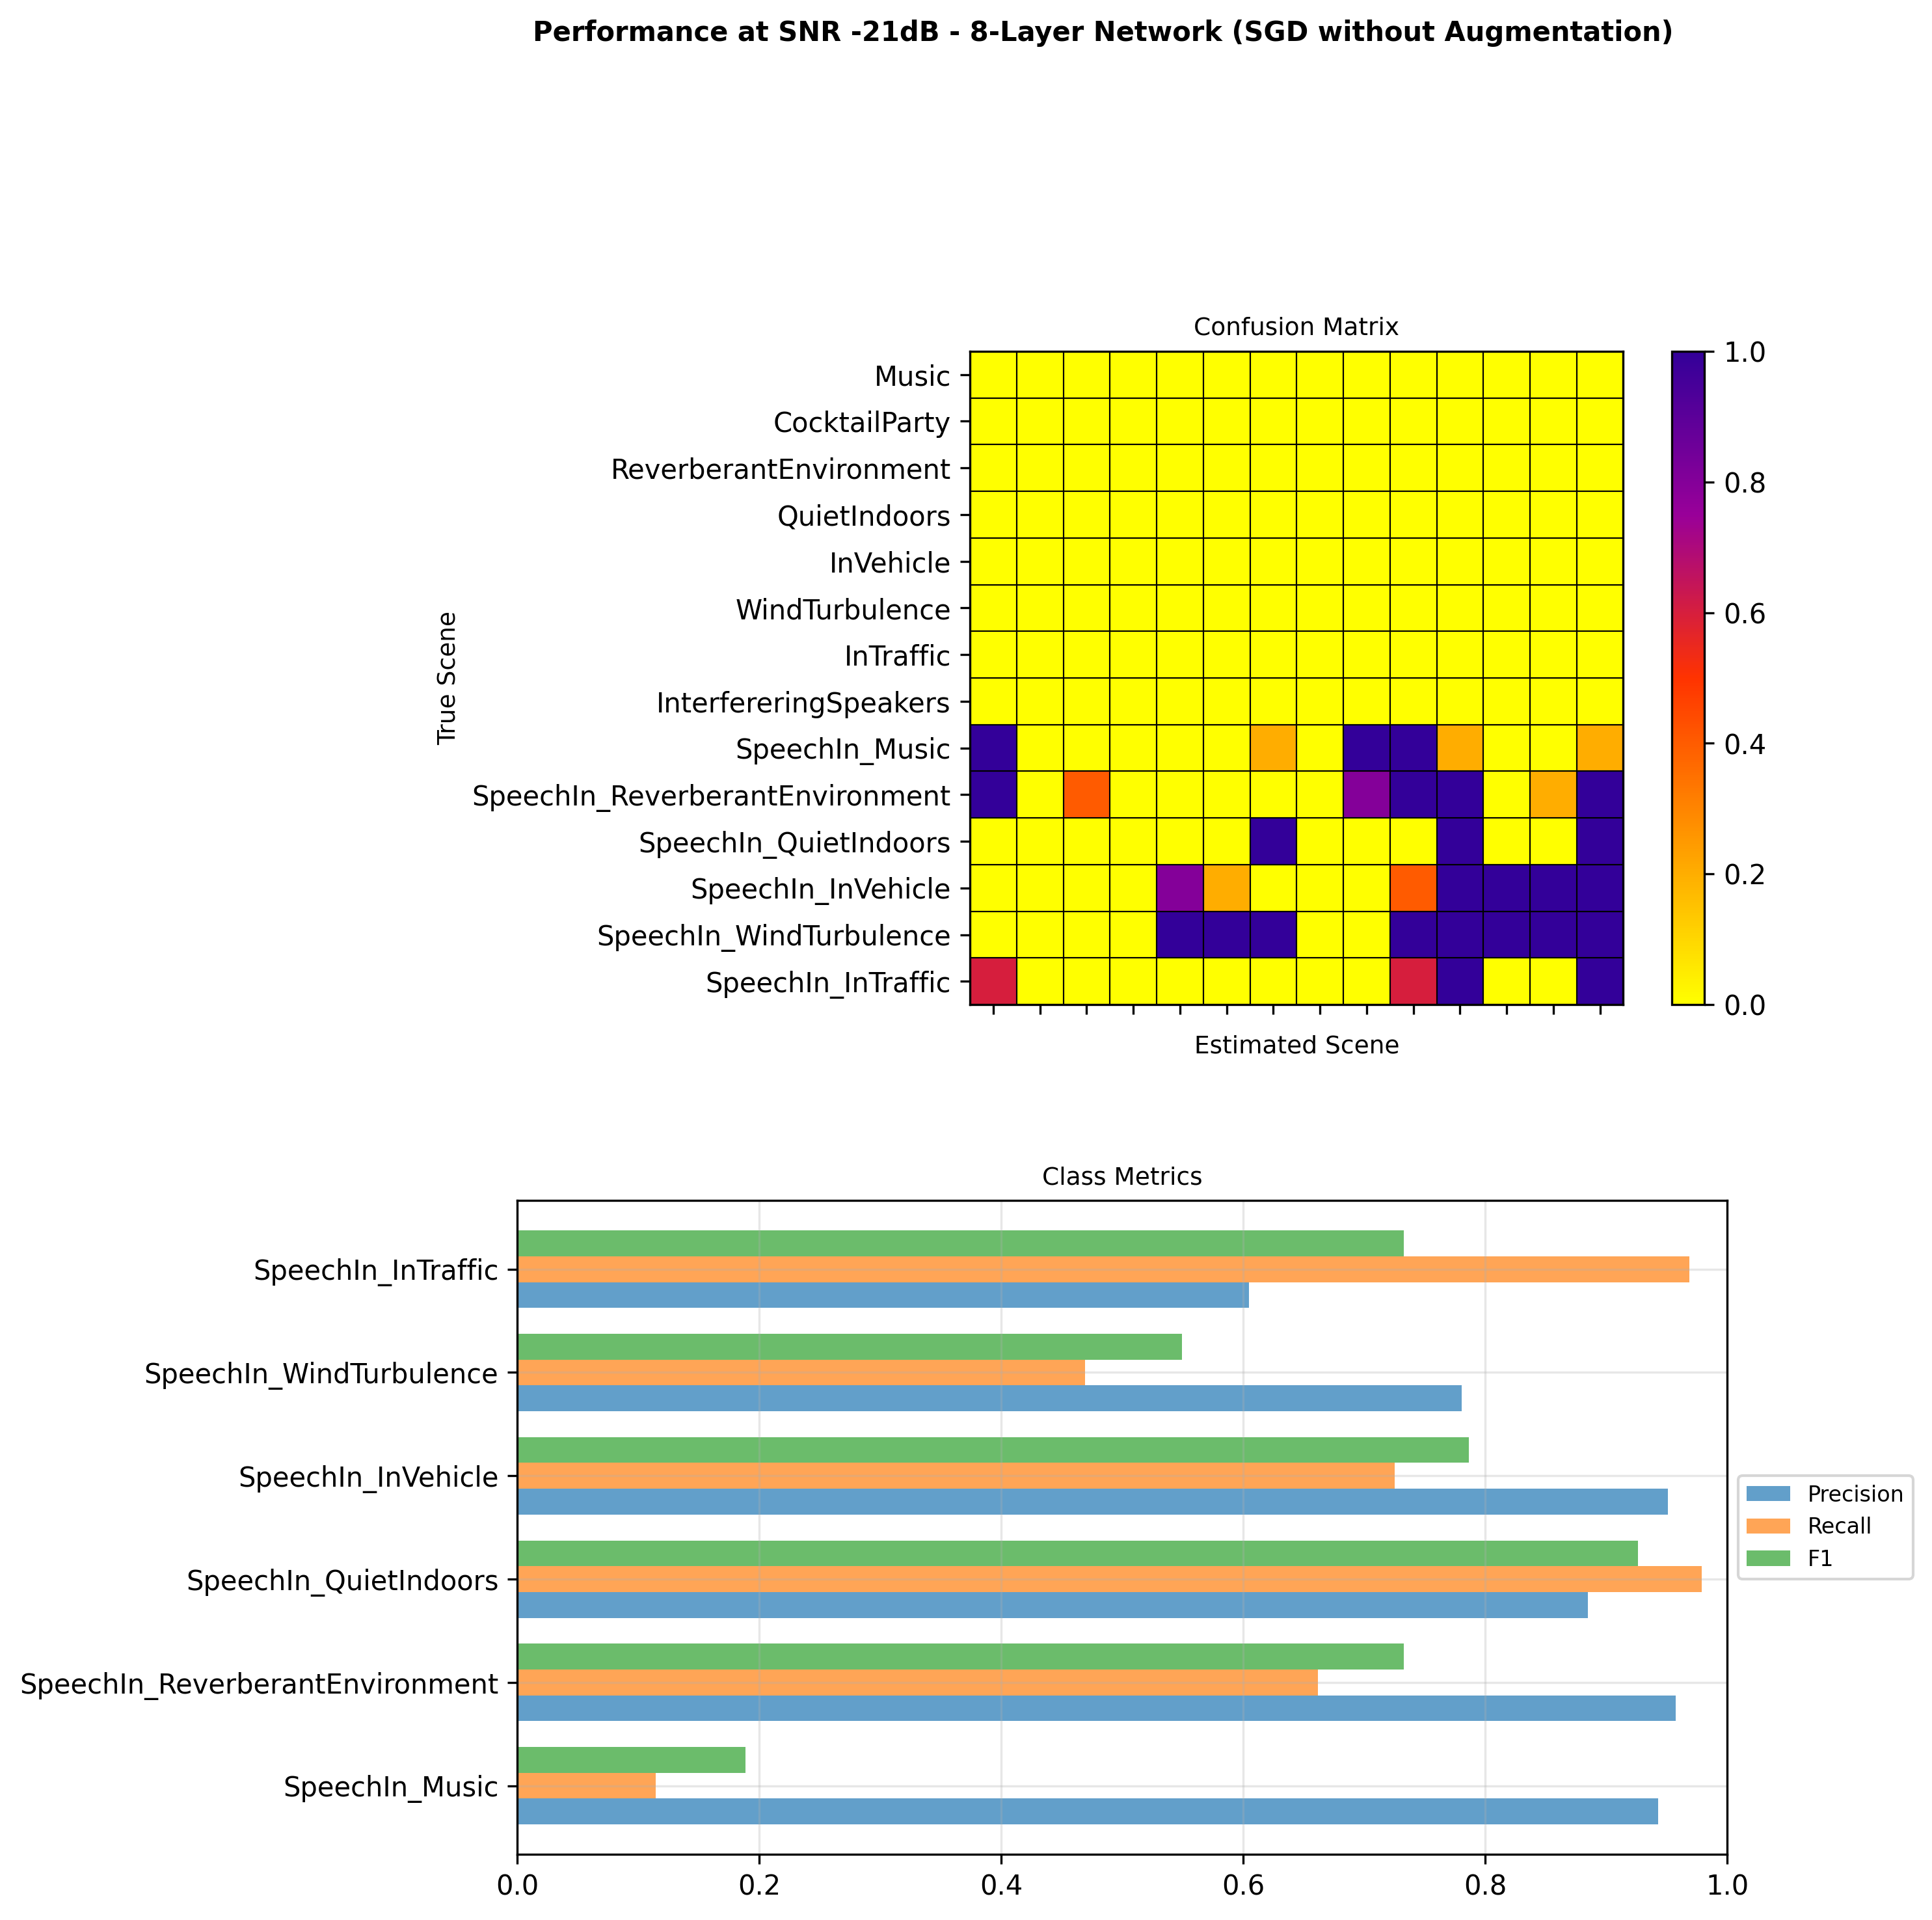
\includegraphics[width=\textwidth]{net-8/FIXED-fixed-lr-sgd/snr_-21_performance.png}
      \caption{}
      \label{fig:fixed-lr-sgd-snr--21}
   \end{subfigure}
   \hfill
   \begin{subfigure}[b]{0.48\textwidth}
      \centering
      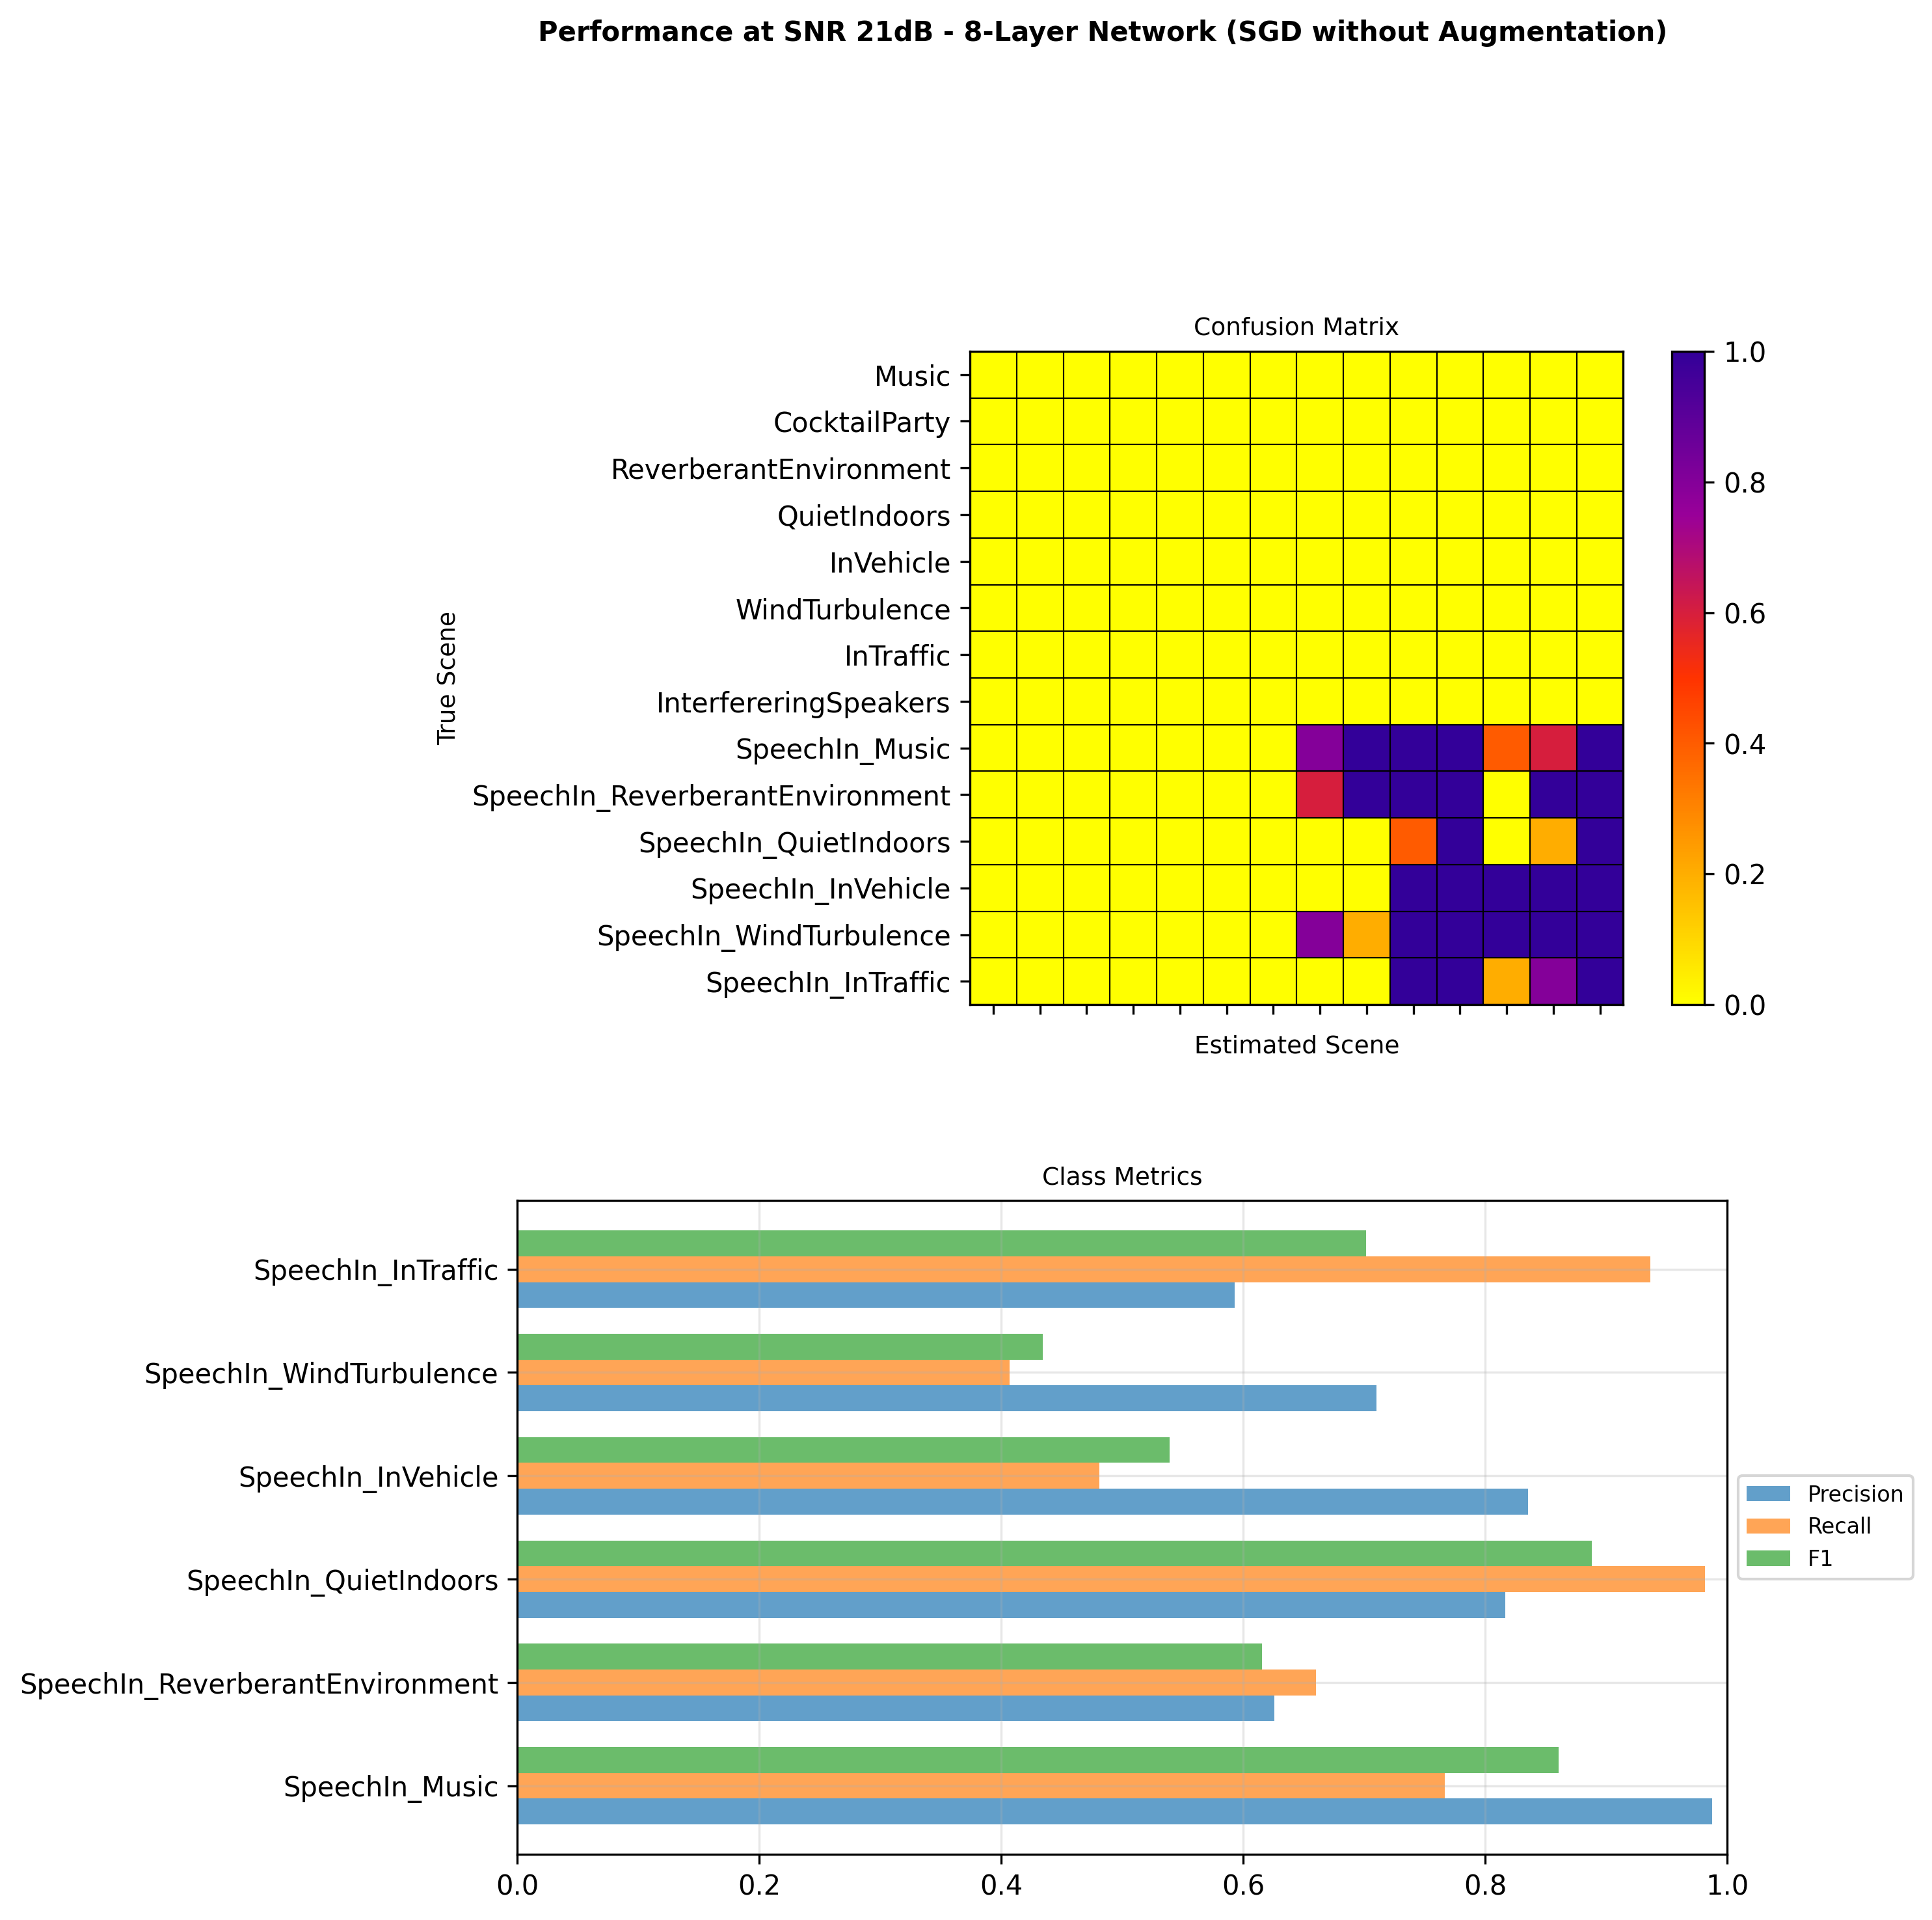
\includegraphics[width=\textwidth]{net-8/FIXED-fixed-lr-sgd/snr_21_performance.png}
      \caption{}
      \label{fig:fixed-lr-sgd-snr-21}
   \end{subfigure}
   \caption{The performance of the net-8 model at SNR -21 (\subref{fig:fixed-lr-sgd-snr--21}) and 21 (\subref{fig:fixed-lr-sgd-snr-21}).}
\end{figure}

Figures \ref{fig:fixed-lr-sgd-snr--21} and \ref{fig:fixed-lr-sgd-snr-21} show 
the performance of the net-8 model at SNR -21 and 21 respectively.
Clearly, the discussed above problems are evident in the results. 
It is interesting to note that in the SNR -21 case, 
the model has a significant precision rate but a low recall rate. 
When paired with the confusion matrix, the model 
is unsure whether to classify the sample as non-speech or speech
which is presumably due to the added difficulty of distinguishing 
between spoken lyrics and speech of a person. 
It is reassuring to see in the SNR 21 case, that the model 
is successfully detecting speech in what is a very noisy environment,
granted it seems to be more conflated in what environment the speech is coming from.

% net-32
\begin{figure}[h]
   \centering
   \begin{subfigure}[b]{0.48\textwidth}
      \centering
      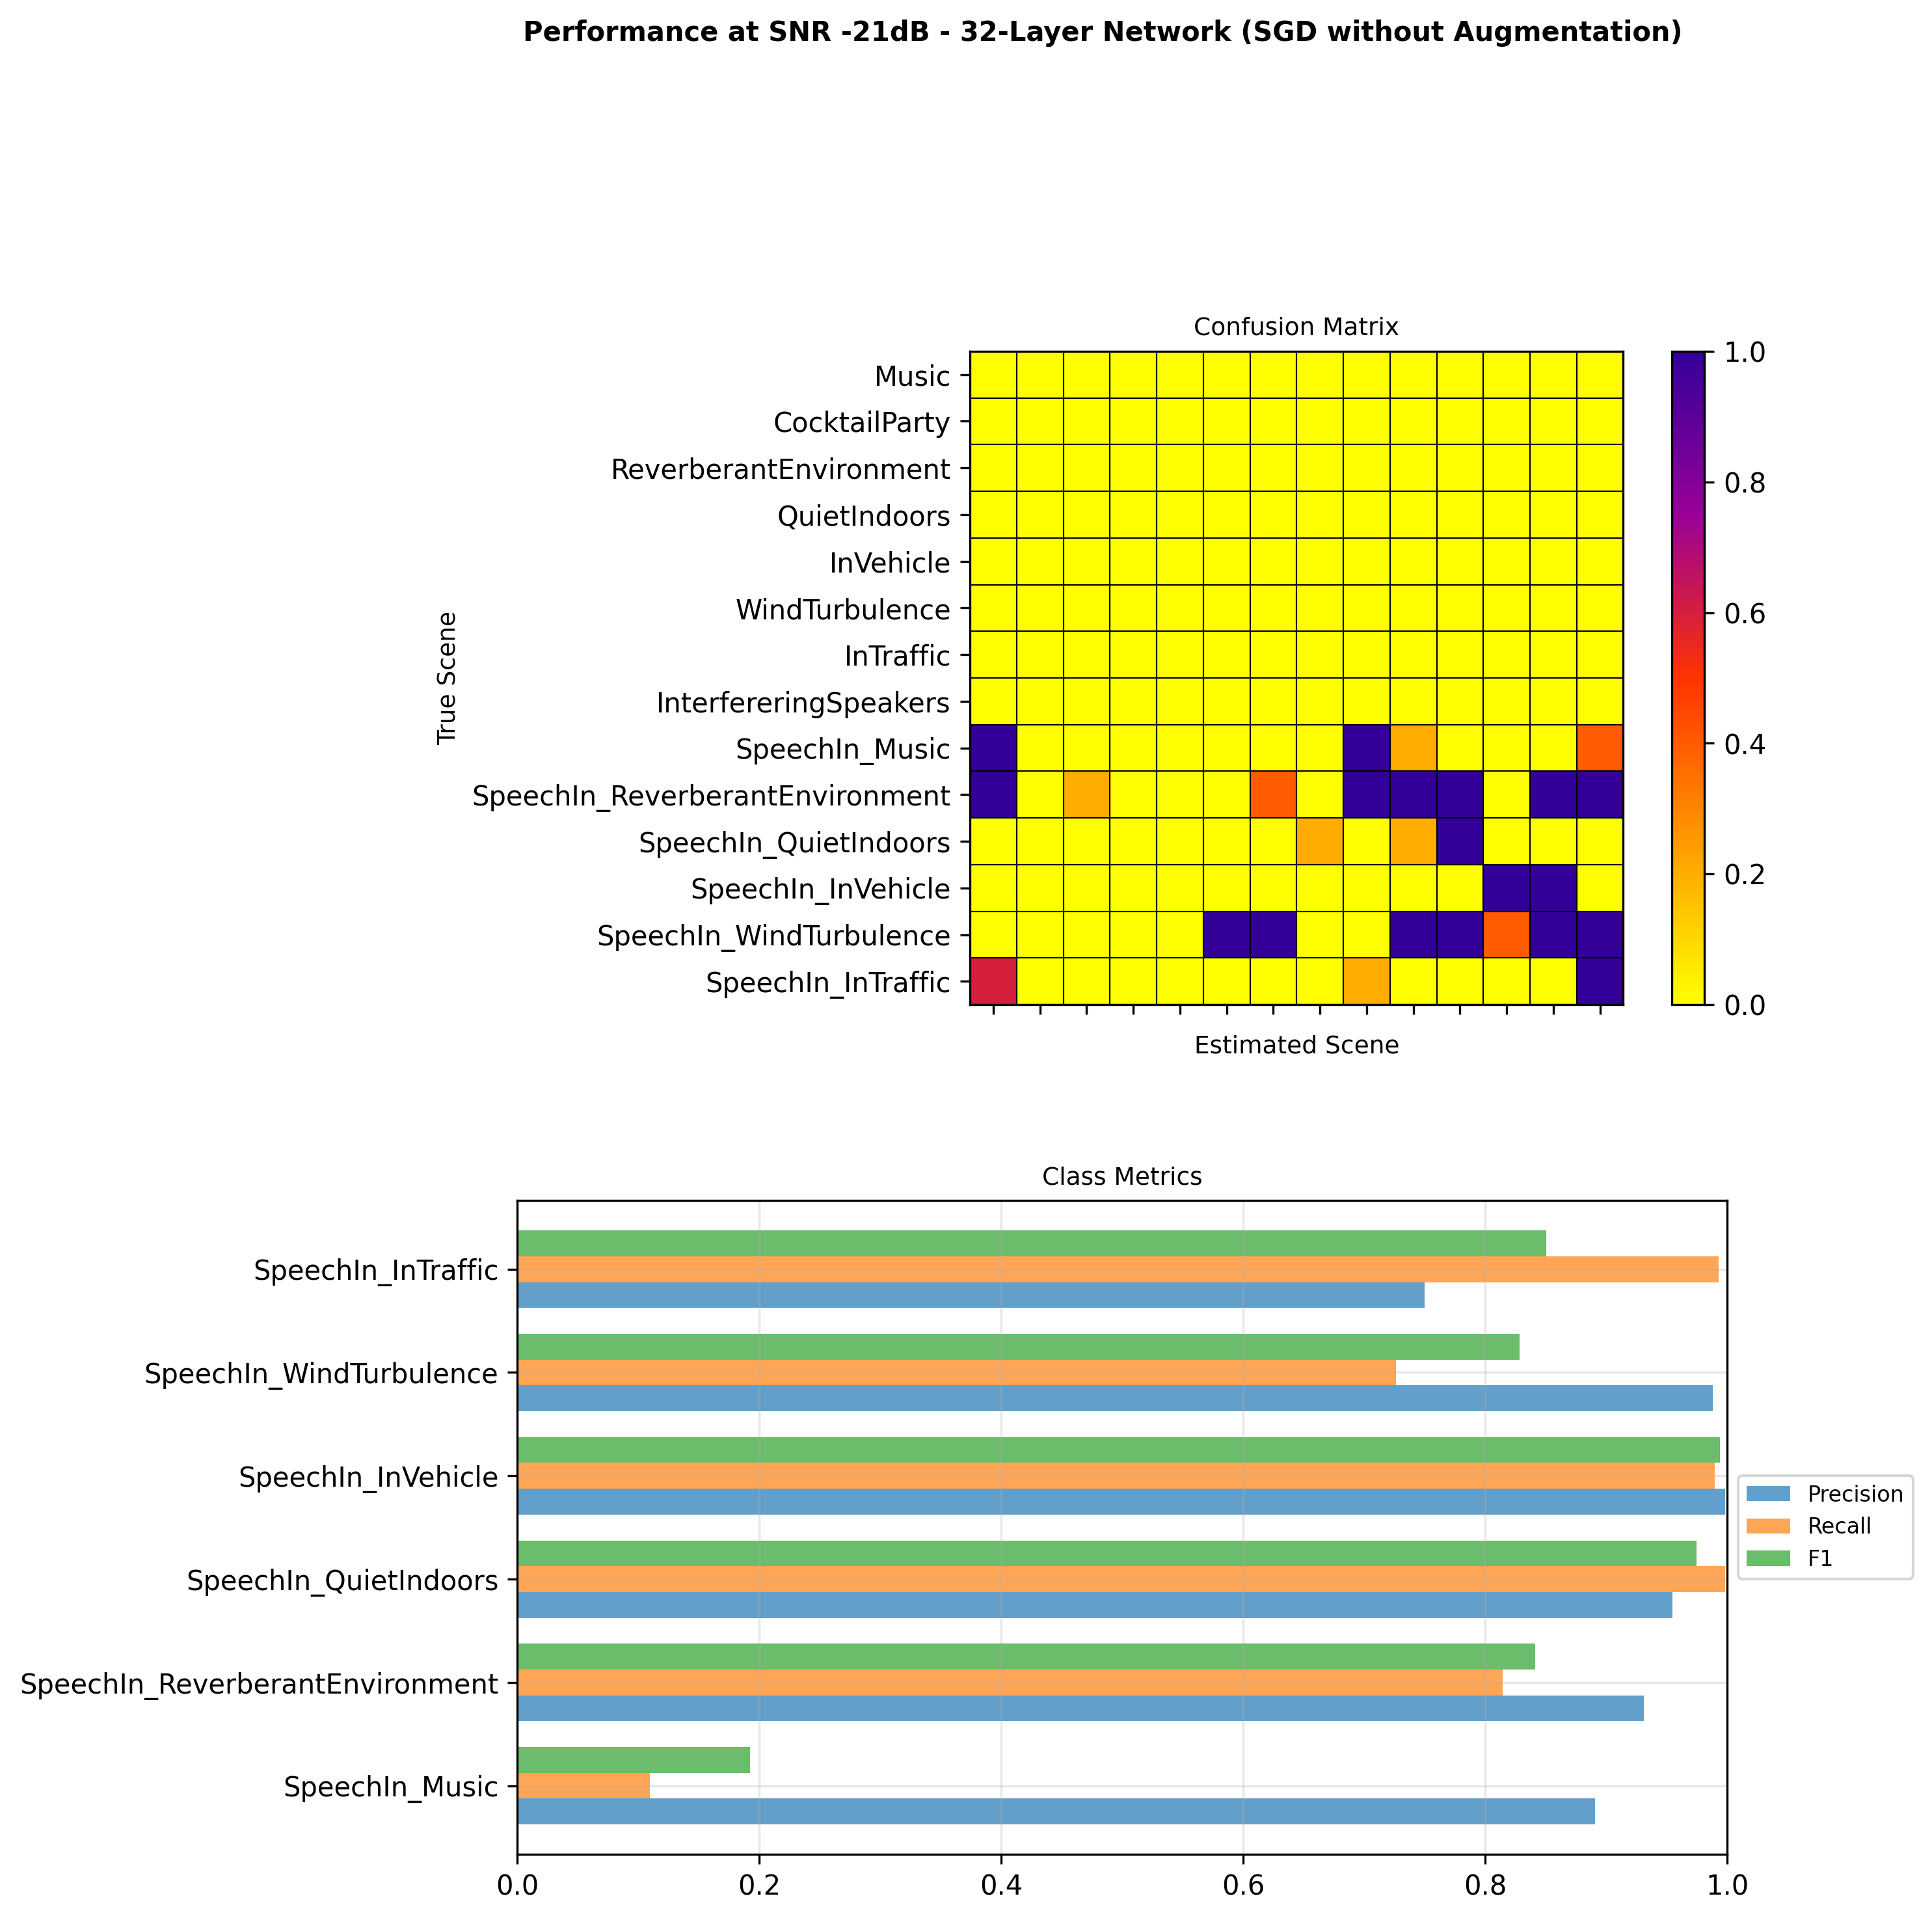
\includegraphics[width=\textwidth]{net-32/FIXED-fixed-lr-sgd/snr_-21_performance.png}
      \caption{}
      \label{fig:fixed-lr-sgd-snr--21-net-32}
   \end{subfigure}
   \hfill
   \begin{subfigure}[b]{0.48\textwidth}  
         \centering
      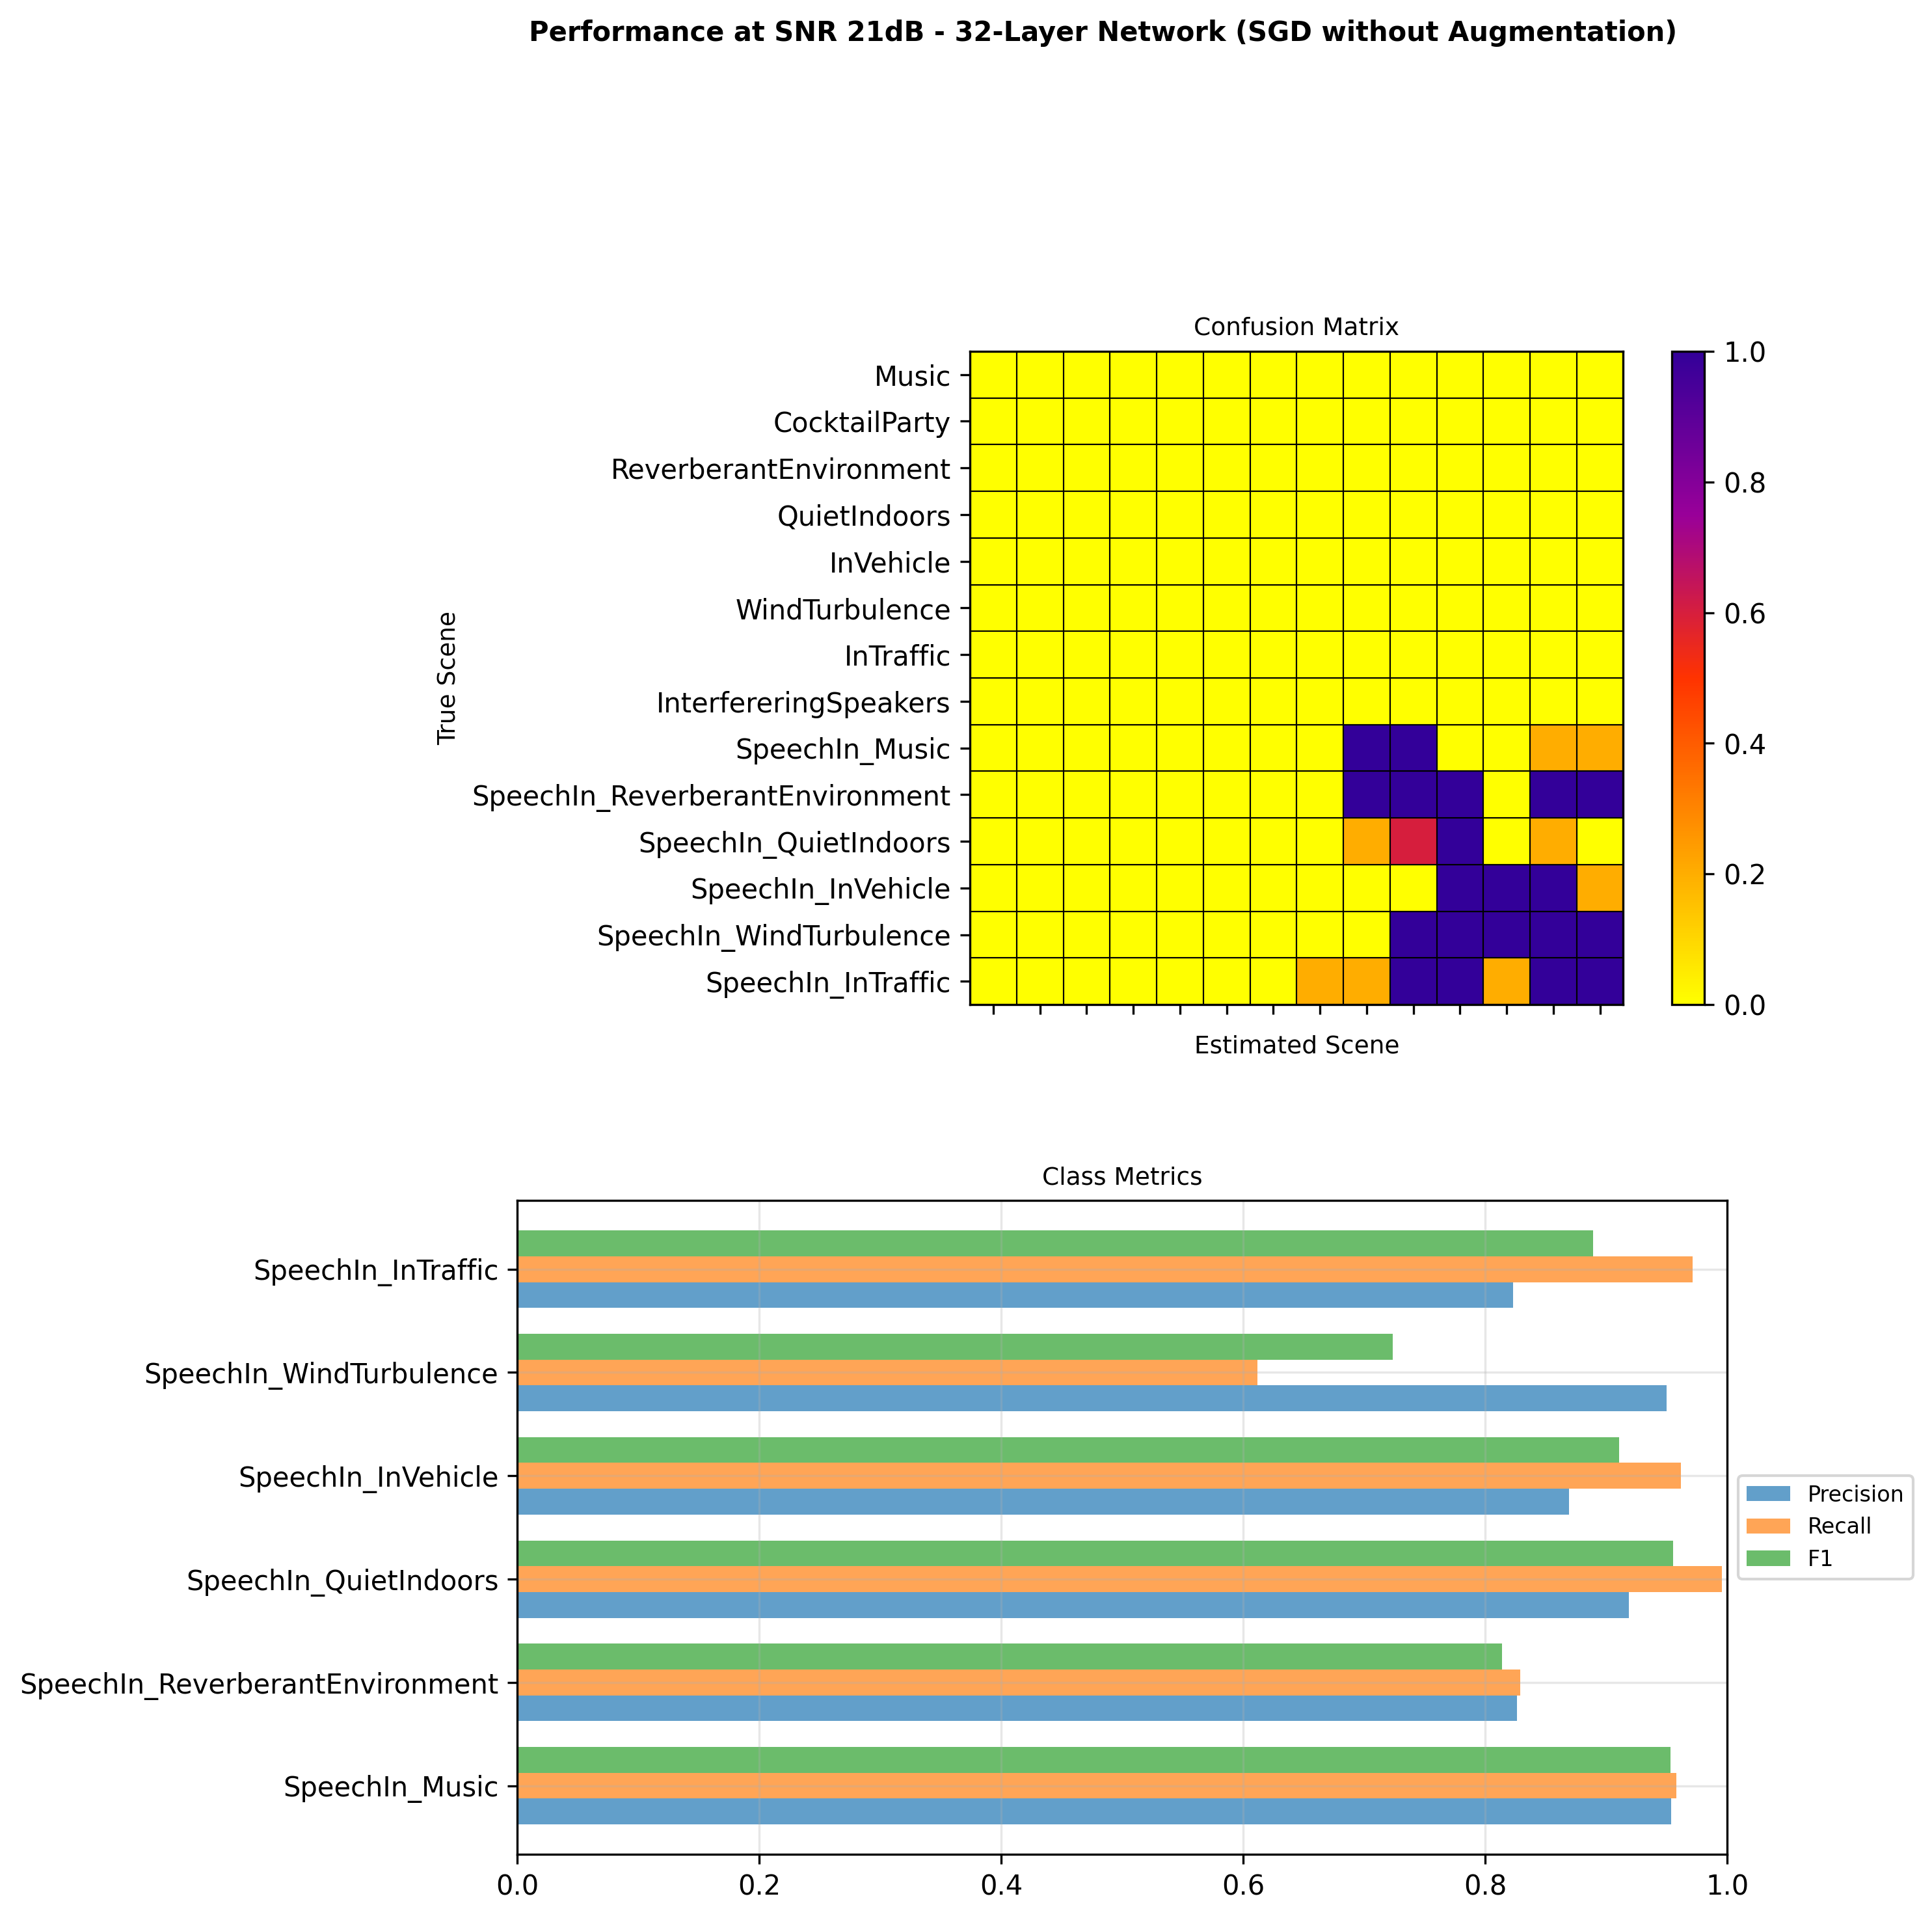
\includegraphics[width=\textwidth]{net-32/FIXED-fixed-lr-sgd/snr_21_performance.png}
      \caption{}
      \label{fig:fixed-lr-sgd-snr-21-net-32}
   \end{subfigure}
   \caption{The performance of the net-32 model at SNR -21 (\subref{fig:fixed-lr-sgd-snr--21-net-32}) and 21 (\subref{fig:fixed-lr-sgd-snr-21-net-32}).}
\end{figure}

Figures \ref{fig:fixed-lr-sgd-snr--21-net-32} and \ref{fig:fixed-lr-sgd-snr-21-net-32} show 
the performance of the net-32 model at SNR -21 and 21 respectively.
In general, the net-32 model is less prone to misclassification, 
as evidenced by the higher F1 scores. However, it is interesting that in the 
net-32 model, the F1 score for Speech in Music is worse than the net-8 model.
Given the complexity of this particular environment, it suggests that 
more work is needed on this particular environment. 

Overall, these more in-depth results not only emphasise 
how difficult the ASA task can be in the presence of speech (especially 
if it is not a binary classification task), but also 
presents a promising direction for further refinement of the model's performance across varying acoustic challenges
in future work.
% The paper also presents the confusion matrix for the net-20 model, and our confusion matrix 
% in Figure \ref{fig:fixed-lr-sgd-confusion-matrix} shows some similarities... TODO: Explain similarities hopefully 

\section{Data Augmentation}
\label{sec:data-augmentation}
\begin{figure}[h]
   \centering
   \begin{subfigure}[b]{0.48\textwidth}
      \centering
      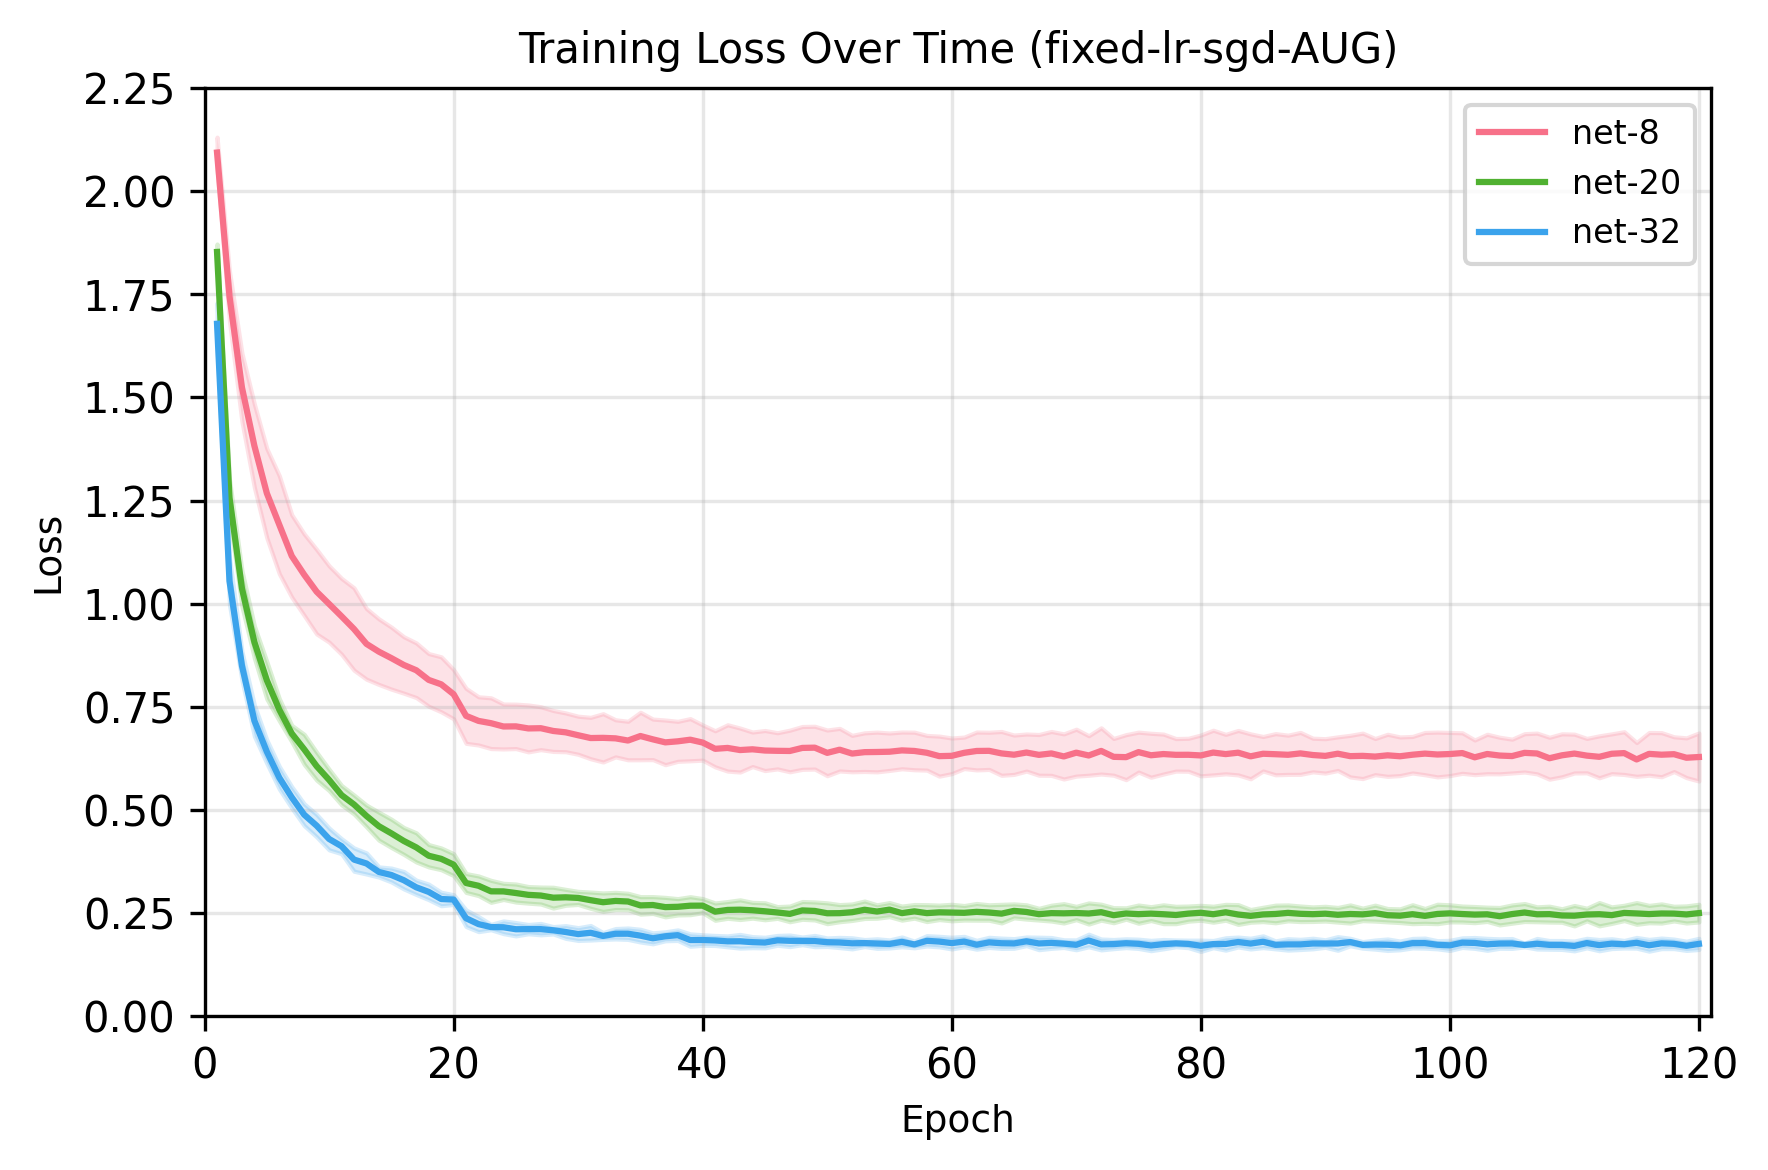
\includegraphics[width=\textwidth]{fixed-lr-sgd-AUG_training_losses.png}
      \caption{}
      \label{fig:data-augmentation-losses}
   \end{subfigure}
   \hfill
   \begin{subfigure}[b]{0.48\textwidth}
      \centering
      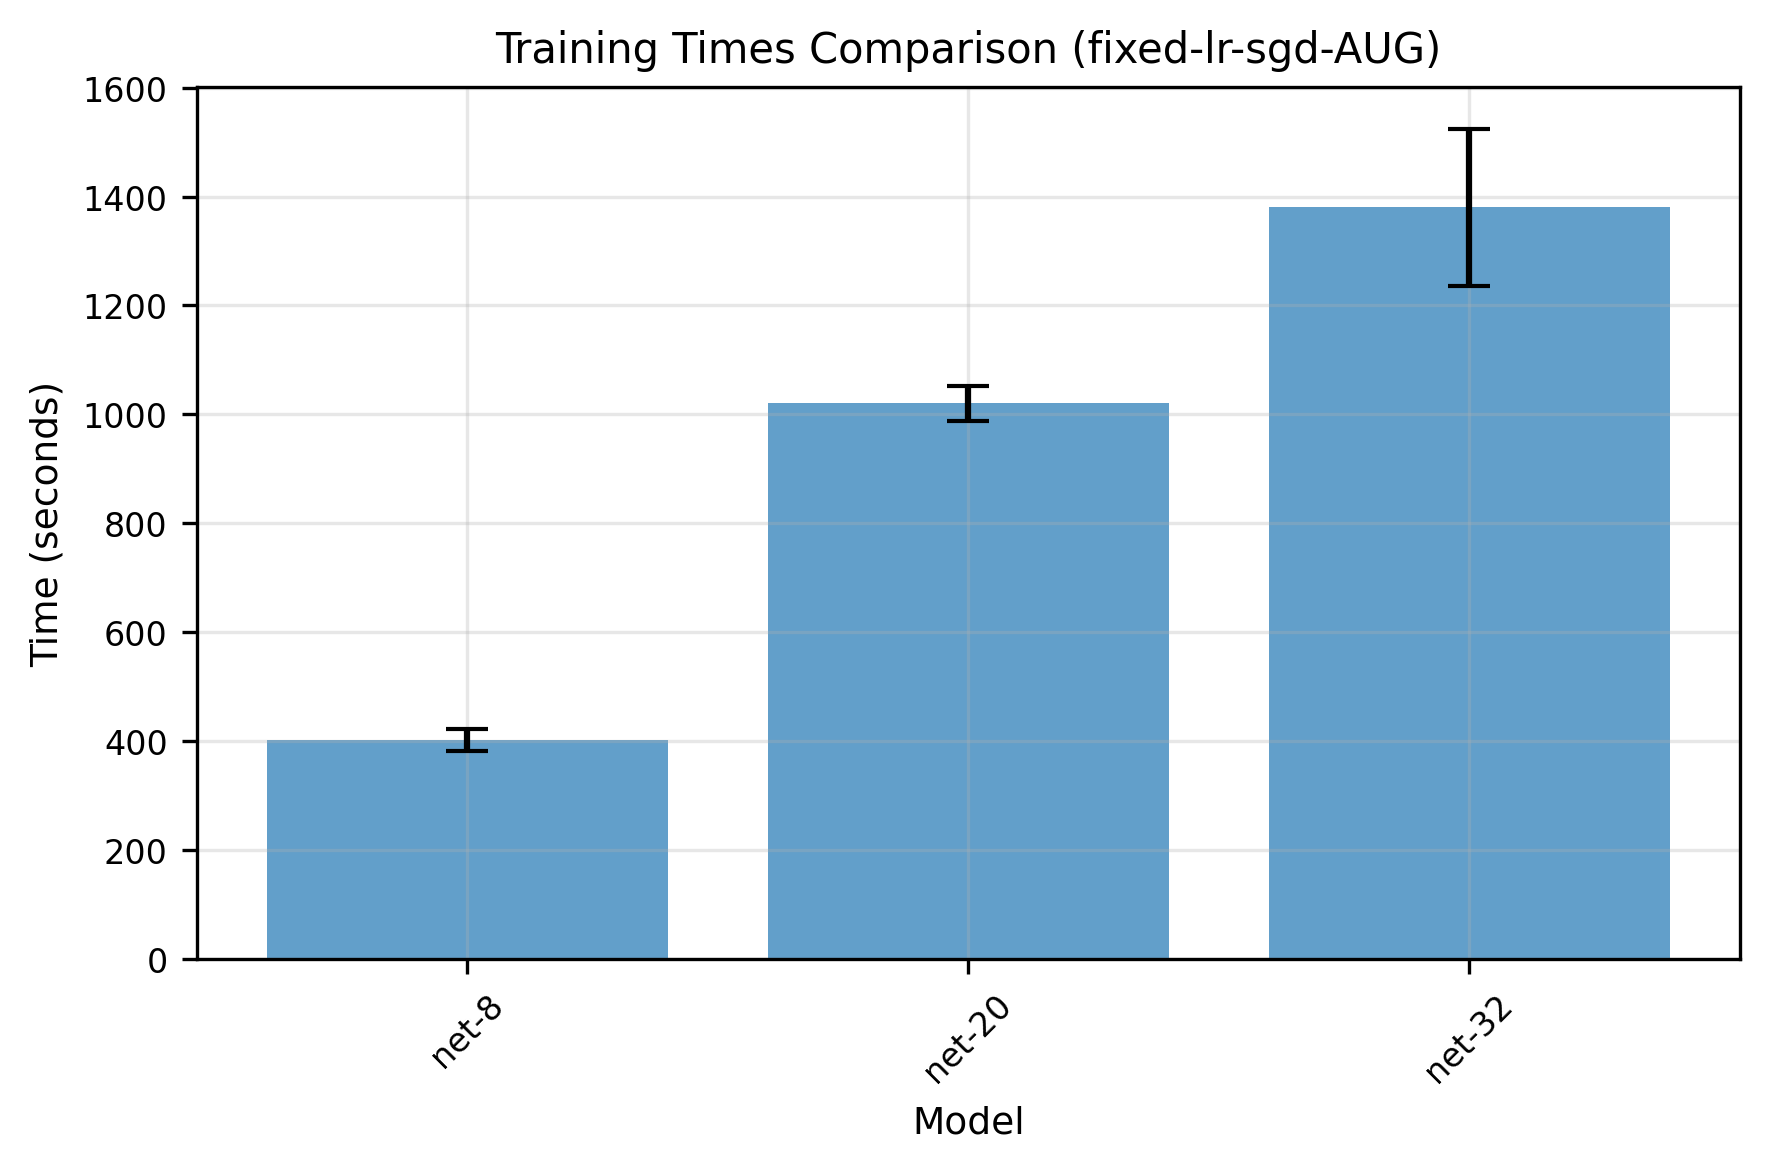
\includegraphics[width=\textwidth]{fixed-lr-sgd-AUG_training_times.png}
      \caption{}
      \label{fig:data-augmentation-times}
   \end{subfigure}
   \caption{The training curves (\subref{fig:data-augmentation-losses}) and training times (\subref{fig:data-augmentation-times}) of the net-8, net-20 and net-32 models when using Data Augmentation.}
\end{figure}
Now that we have a baseline, the next step is to test the hypothesis 
that utterance-level data augmentation is effective. More specifically, 
notice that in the baseline, per epoch, we are training the model on all 
combinations of SNRs, which in the case of 15 SNRS, means for each sample,
per epoch we need to do 15x the amount of work. From a training perspective, 
this means that the model will take longer to train. Instead, we wanted 
to see if we can not only reduce the amount of work per epoch, but also 
improve the performance of the model.

We still precompute the spectrograms before training, however, during 
training, each sample is stochastically assigned an SNR from the set of 
15 SNRS. We do an equal weighted random sampling from the set of SNRS 
and perhaps to better mimic the distribution of the sounds, it might 
be better to use a weighted sampling. We leave this as 
potential future work.

Figures \ref{fig:data-augmentation-losses} and \ref{fig:data-augmentation-times} show 
the resulting training curves and training times for the net-8, net-20 and net-32 models
when now using the data augmentation approach. The plateau of the training curves 
is similar to the baseline, but the training times have at least 
5-fold reduction. While the cross entropy loss is higher, this is 
to be expected as there are less samples during training and since the formula for 
Cross-Entropy loss is a weighted sum of the negative log likelihood of 
the correct class, a lower number of samples means that the loss 
will be higher. When we look at the test accuracy (Figure \ref{fig:data-augmentation-accuracies}),
we see that there is no significant difference in the performance of the model 
but the training time has been reduced by a factor of 5.

\begin{figure}[h]
   \centering
   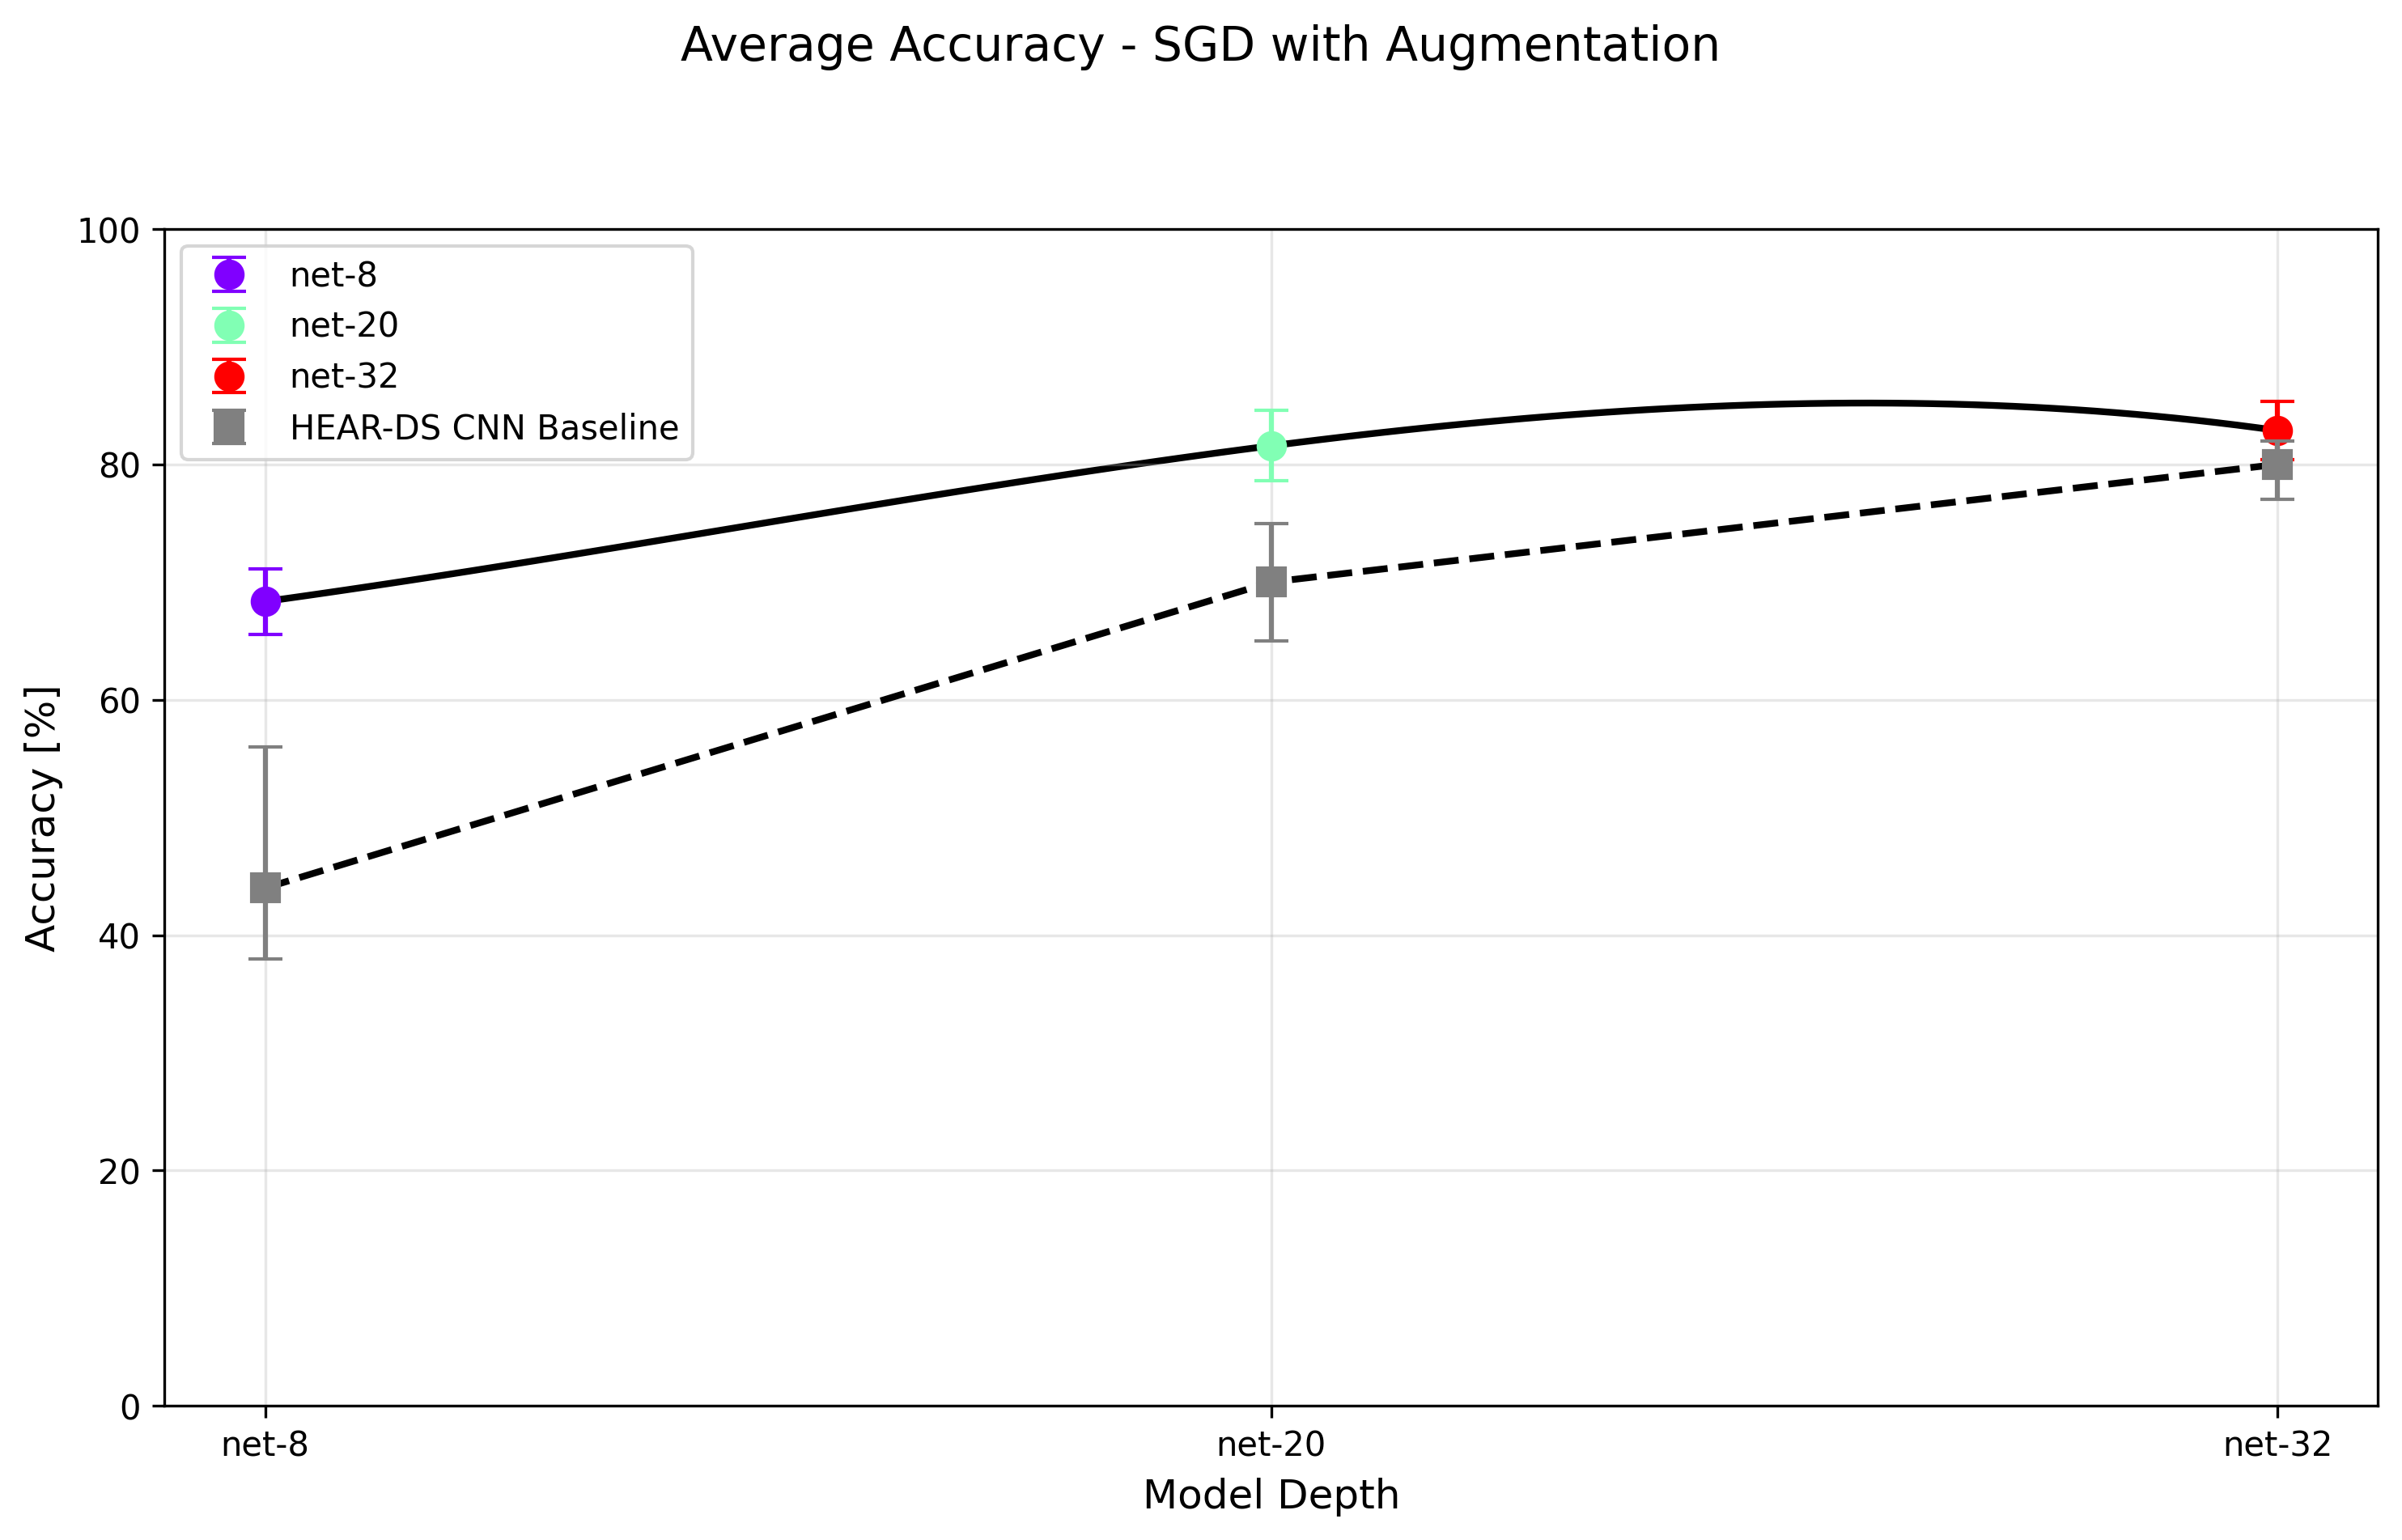
\includegraphics[width=0.8\textwidth]{average_accuracies_sgd_aug.png}
   \caption{The average accuracies fitted with linear regression of the net-8, net-20 and net-32 models when using the fixed learning rate SGD approach with data augmentation.
   Also plotted are the extrapolated results from \citet{Huwel2020HearDS} for the three models.
   }
   \label{fig:data-augmentation-accuracies}
\end{figure}
% three models, and this is a good time to point out that the loss 
% will be higher for the data augmentation approach. This is expected 
% as there is less samples during training and since the formula for 
% Cross-Entropy loss is a weighted sum of the negative log likelihood of 
% the correct class, a lower number of samples means that the loss 
% will be higher. However, when we have a look at the test accuracy (Figure \ref{fig:data-augmentation-accuracies}),
% we see that the data augmentation approach is actually better than 
% the baseline. This is a good sign and suggests that the data 
% augmentation approach is effective. Figure \ref{fig:data-augmentation-confusion-matrix} shows 
% that the model is less ...

\section{Adam Optimiser Approach}
Since we established that the data augmentation approach is effective, we wanted to see 
if the use of a different optimiser would yield better performance or reduce the 
training time. Additionally, since we noticed in the earlier experiments 
that the model was converging much earlier than the 120 epochs (let alone the suggested 
240 epochs), thus we wanted to adopt an early stopping approach as well.
\citet{Huwel2020HearDS} mentions that the use of Adam is sensitive to the initialisation 
and so they they opted for the SGD approach. 
They back this up with a paper by \citet{} 
but after reading it, while it says 
Adam can lead to poor convergence in `\textit{some settings}'
so it would have been interesting to see from \citet{Huwel2020HearDS}
to see if this is the case for the ASA task. As such, 
we will be taking this forward to investigate this.


\begin{figure}[h]
   \centering
   \begin{subfigure}[b]{0.48\textwidth}
      \centering
      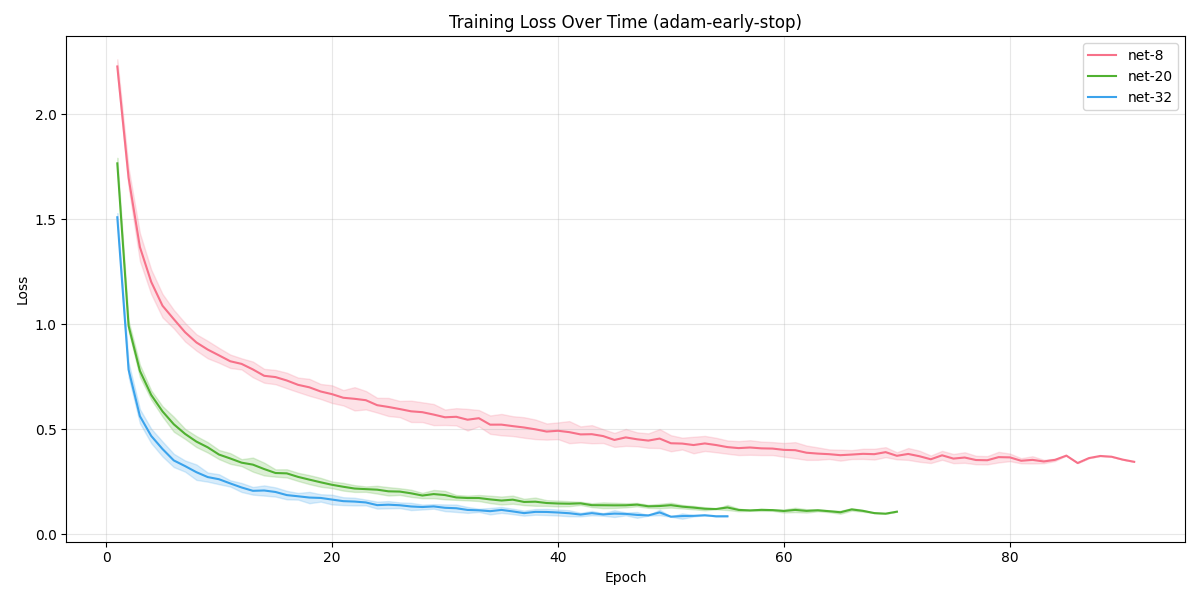
\includegraphics[width=\textwidth]{adam-early-stop_training_losses.png}
      \caption{}
      \label{fig:adam-optimiser-losses}
   \end{subfigure}
   \hfill
   \begin{subfigure}[b]{0.48\textwidth}
      \centering
      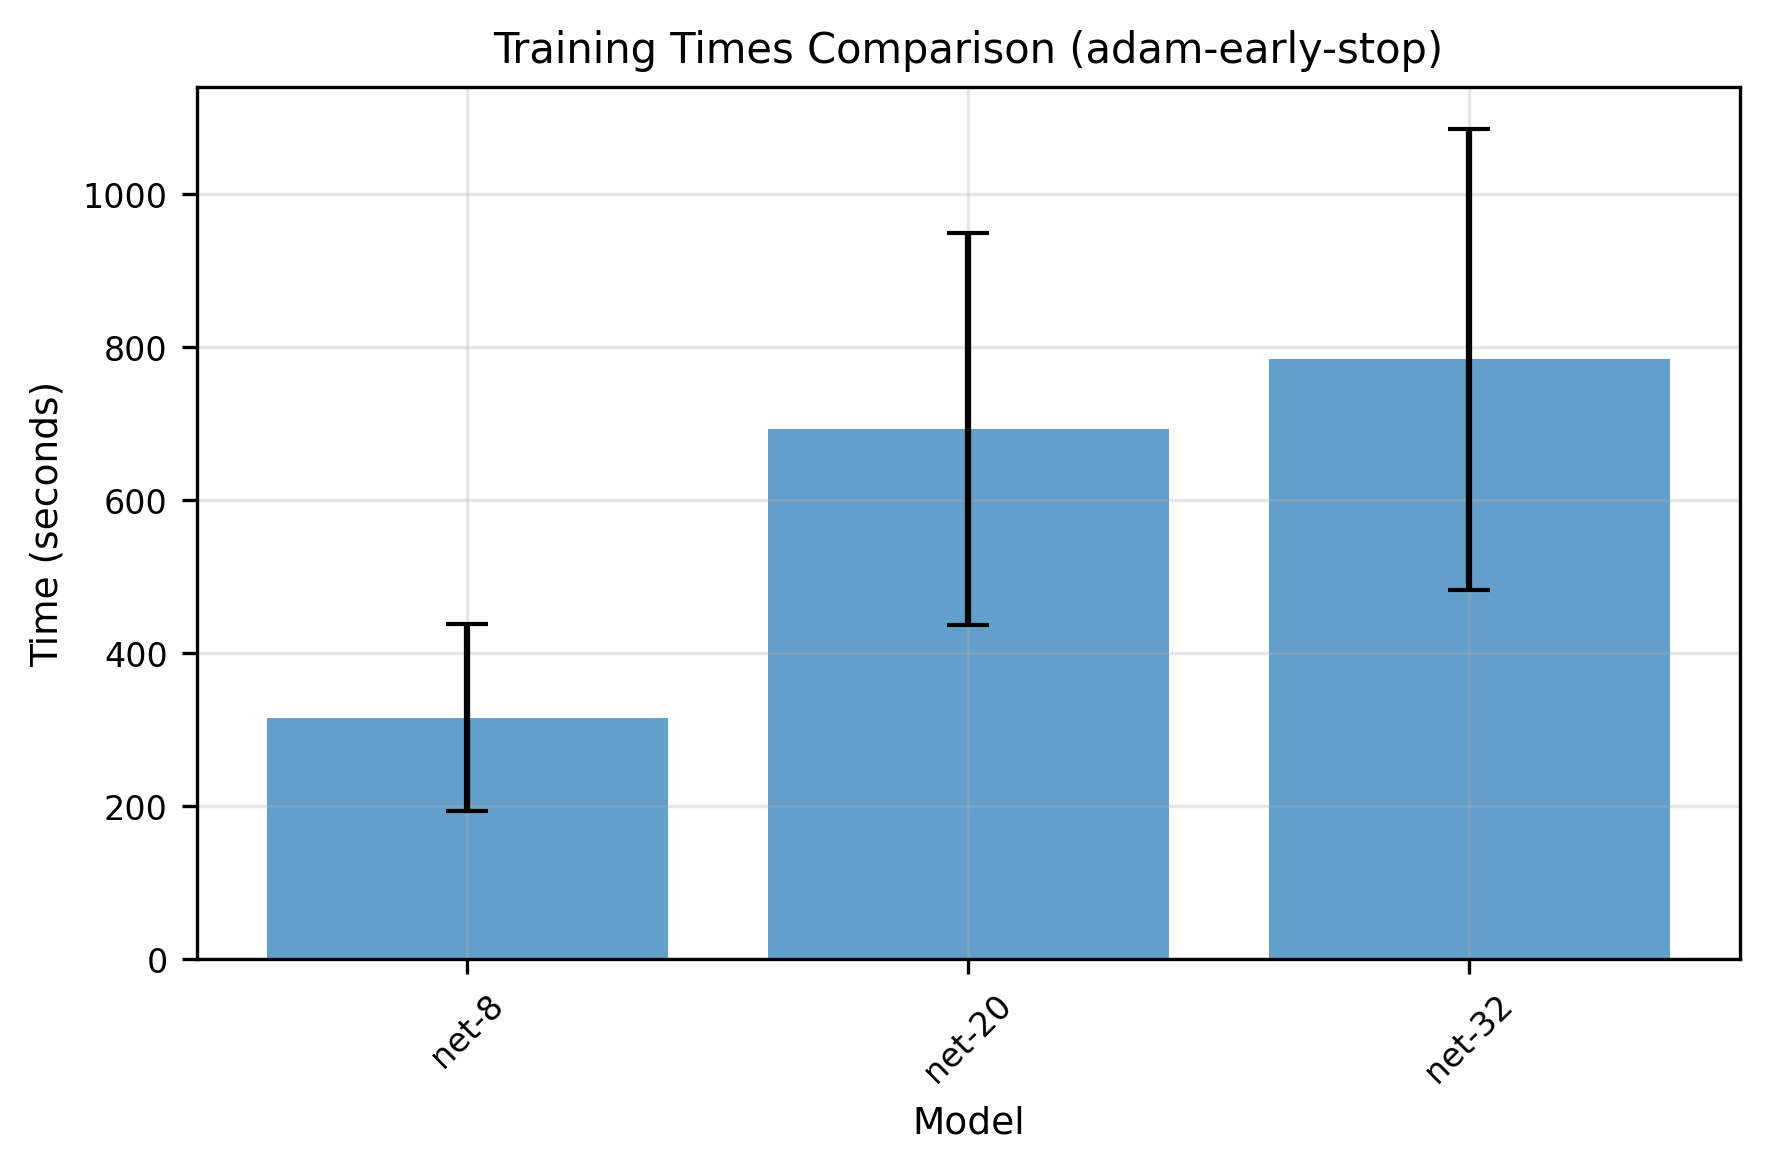
\includegraphics[width=\textwidth]{adam-early-stop_training_times.png}
      \caption{}
      \label{fig:adam-optimiser-times}
   \end{subfigure}
   \caption{The training curves (\subref{fig:adam-optimiser-losses}) and training times (\subref{fig:adam-optimiser-times}) of the net-8, net-20 and net-32 models when using the Adam optimiser.}
\end{figure}

Figure \ref{fig:adam-optimiser-losses} and \ref{fig:adam-optimiser-times} shows 
the training curves and training times for the net-8, net-20 and net-32 models
when using the Adam optimiser. We can see that the training curves converge to a 
loss similar as to the one in \ref{sec:data-augmentation}, but the training times 
are in some cases reduced by 50 \%, which is due to the early stopping approach.
While there seems to be evidence of this sensitivity (as observed by the slightly larger spread 
of the training curves), it is not as pronounced as the paper suggested and 
could possibly suggest that the setting this optimiser is being used 
is not as bad. 

\section{Validating against TUT Acoustic Scenes 2016}
\begin{figure}[h]
   \centering
   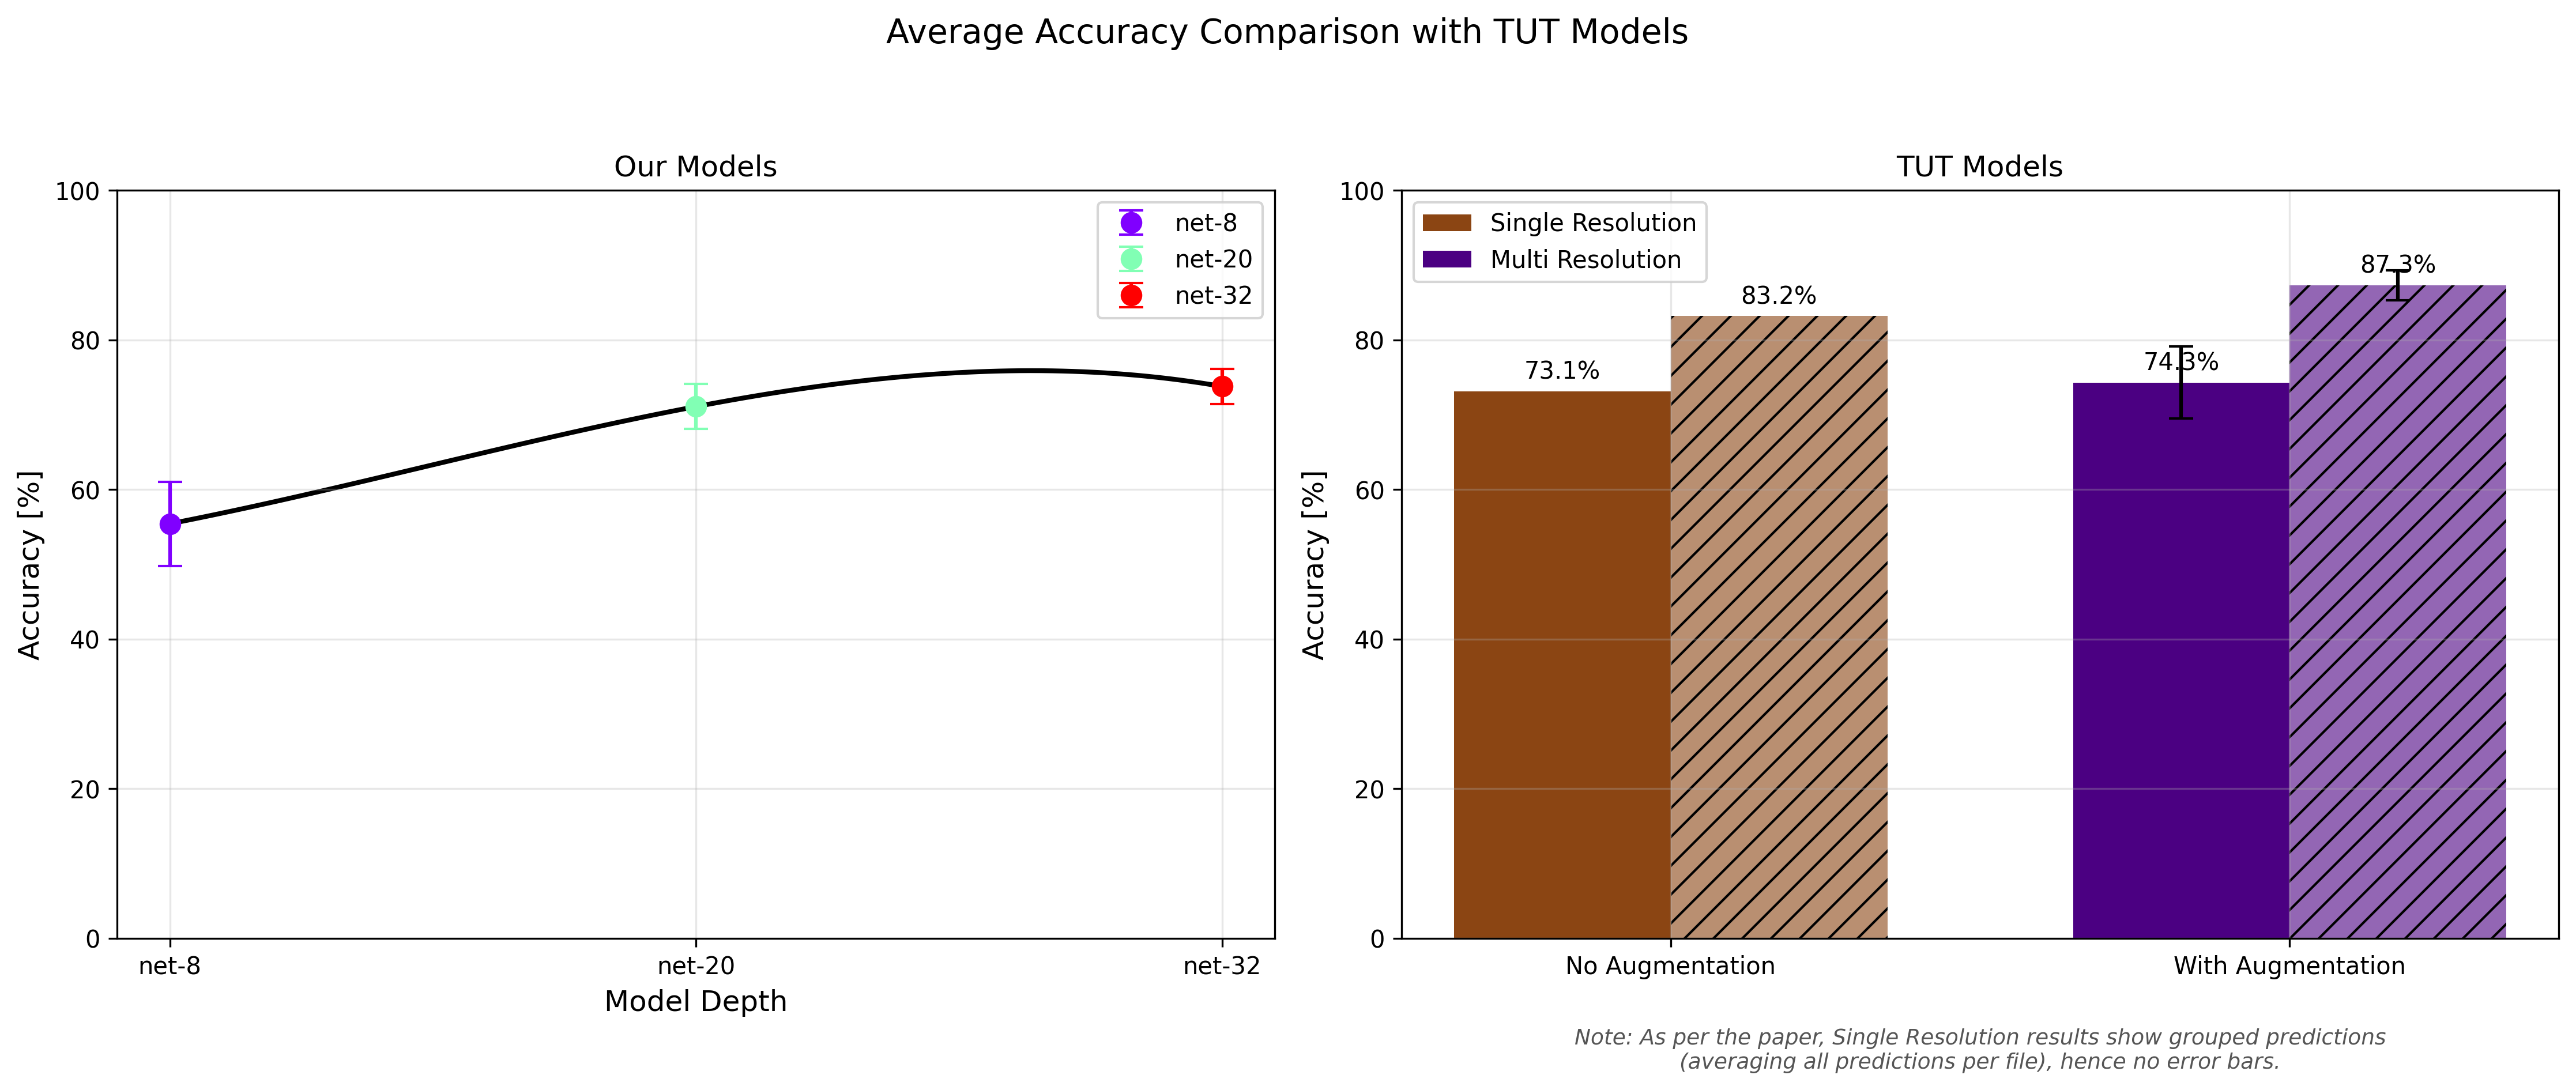
\includegraphics[width=0.9\textwidth]{average_accuracies_tut_comparison.png}
   \caption{(left) The average accuracies fitted with linear regression of the net-8, net-20 and net-32 models when using the Adam optimiser. 
   (right) Various models extrapolated from Table 2 of \citet{schindler_multi-temporal_2018} for comparison.}
   \label{fig:tut-asa-results}
\end{figure}
As a means of validating that the implementation is correct, 
we wanted to see if we can get results similar to those of a paper 
that is doing ASA. In particular, we will be using the paper by 
\citet{schindler_multi-temporal_2018}. It uses the TUT Acoustic Scenes 2016 dataset
as described in Section \ref{sec:datasets}.

Figure \ref{fig:tut-asa-results} shows two accuracy curves, one for our results 
and one for the results from \citet{schindler_multi-temporal_2018}. For their results, 
we reported two models, the single resolution model, which is their baseline, 
and the multi-resolution model, which is their proposed model. They also 
report results with and without augmentation, though their augmentation techniques 
are going to be different from ours as our data augmentation technique is more 
concerned with the speech mixing process whereas theirs is a more general 
data augmentation technique and they utilise techniques such as pitch shifting and 
time stretching to name a few. However, we leave it for future work 
to perhaps adopt their data augmentation techniques and see 
if we can get huge improvements in performance as can be seen in their results.
Nevertheless, it is encouraging to see 
that the net-32 model is able to just about match the performance of the single resolution model 
without augmentation, as it indicates our implementation is fundamentally sound. Additionally, we 
leave it for future work to adopt the multi-resolution model into our framework and see 
if we can get any improvements in performance.

\section{Feasibility} 
We tested the feasibility of the task from a HA perspective by benchmarking 
the model's parameter count and required floating point operations [FLOP(s)].
Contrast this with FLOPs which is the number of FLOP(s) per second. Based on 
FLOP(s) and FLOPs, we can calculate the theoretical inference time of the model.
Table \ref{tab:model-comparison} shows the results for the net-8, net-20 and net-32 models.
Given that the state of the art models of HAs have capabilities of 
7,700 million FLOPs and models with 5 million parameters, our models are well within these limits.
The theoretical inference times would all be well below the acceptable latency for HAs.
Future work would be to investigate on a low-power device that has capabilities 
similar to that of HAs. 

\begin{table}[h]
   \centering
   \begin{tabular}{lccc}
      \toprule
      Model & FLOP(s) Count & Parameters & Theoretical Inference Time\footnotemark \\
      \midrule
      net-8 & 13.550M & 7.951K & 1.759 ms \\ % 0.0017597403 seconds
      net-20 & 52.694M & 46.423K & 6.753 ms \\ % 0.0067532468 seconds 
      net-32 & 114.421M & 116.623K & 14.805 ms \\ % 0.0148051949 seconds
      \bottomrule
   \end{tabular}
   \caption{{Comparison of the FLOPs and parameters of the net-8, net-20 and net-32 models.}}
   \label{tab:model-comparison}
\end{table}
\footnotetext{{Assumes a 7,700M FLOPs capable device and that the formula in \ref{eq:inference-time} is used.}}

\chapter{Speech Enhancement Experiments}
\label{chap:se-experiments}
We split the chapter into three parts. We first outline the data preparation processs 
and the deviations done from the ASA task. We then present the results of the speech 
enhancement task in the \heards dataset. Afterwards, as a means of validation, we 
validate the model in the \vbd dataset and compare the results from 
\citet{kim_specmix_2021}. Lastly, just as we did for the ASA task, we will 
discuss the feasibility of the task from a HA perspective.

\section{Data Preparation}
We for the most part incorporated the same data preparation approach as the ASA task, so consult Section \ref{sec:data-preparation} for 
more in-depth detail. The differences deviate in the feature transformation, 
since we will now not use the logmel transformation, but instead use the standard 
spectrogram. It is worth noting that in \vbd, the samples 
are mono, so we use them as is, but in \heards, the samples are dual channel (left and right, microphones), 
so for exploration we just use the left channel. In a deployment scenario, we would train two models, one for the left 
and one for the right channel, and use the respective model on the respective HA device.
% Furthermore, the requirement to store at least twice as many samples necessitates a proportional increase in memory capacity. Memory usage scales linearly with the number of SNR levels. Training on 15 SNR levels, as was done for the ASA task, proved infeasible for the present dissertation. Consequently, the speech signal was mixed with background noise at only 5 SNR levels—\([-10, -5, 0, 5, 10]\) dB—in order to avoid IO bottlenecks and degradation during model execution, given that the waveforms are stored in memory. For context, even with 5 SNR levels, approximately 50 GB of memory was required for the HEAR-DS training set. Although this range provides a robust basis for evaluating model performance, future work could investigate the impact of incorporating a broader range of SNR levels.
Additionally, the need to load both the noisy and clean speech signals 
during training, means that twice as much memory is needed compared to the ASA task.
So training on 15 SNR levels was not feasible for this task 
in this part of the dissertation. As such, we only 
mix the speech signal with the background noise at 5 SNR levels - [-10, -5, 0, 5, 10] dB.
To speed up training by reducing the IO bottleneck, we preload the waveforms into memory 
rather than loading them on demand. So even with 5 SNR levels, 
50 GB of memory is required for the training set for the \heards dataset.
For future work, it would be interesting to see how the model performs with 
more SNR levels.

The Adam optimiser was used with a learning rate of 0.0006 and a batch size of 16.
Early stopping was applied when the loss did not improve after 5 epochs.
At each epoch, we employ a similar data augmentation approach as the ASA task, 
namely, for each sample, we randomly pick a SNR level and mix the speech signal with the background noise 
at that SNR level. 

% \section{One Model Approach}
% This is where we train a single model to enhance speech in all environments. 

% Training Curve
% STOI PESQ per SNR Table (Poorer results after enhancement)
% Despite this, comparing the clean, noisy and enhanced spectrograms, we can see that the enhanced 
% spectrogram is removing the noise, but the speech is degraded which can be noted by the discontinuity in the formants 
% 

\section{HEAR-DS Results}
We created five train+test splits of the \heards dataset as in the ASA task to obtain a 
more in depth analysis of the model's performance. Since there 
are 6 speech environments, we trained 6 SE models, one for each environment. 
Since there are a different number of samples for each environment, 
the convergence of the training curves are different. 
It is worth noting that for \heards all of the samples are 10s long,
so during testing we also use 10s samples. Investigating 
the performance at shorter time segments is left for future work.

Figure \ref{fig:hear-ds-training-curves} shows the training curves for the 
6 SE models. Notably compared to the ASA task, the training curves for each 
environment have more variance, which could be for numerous reasons, such 
as the initialisation of weights being an important factor. We leave this 
for future work to investigate.

\begin{figure}[h]
   \centering
   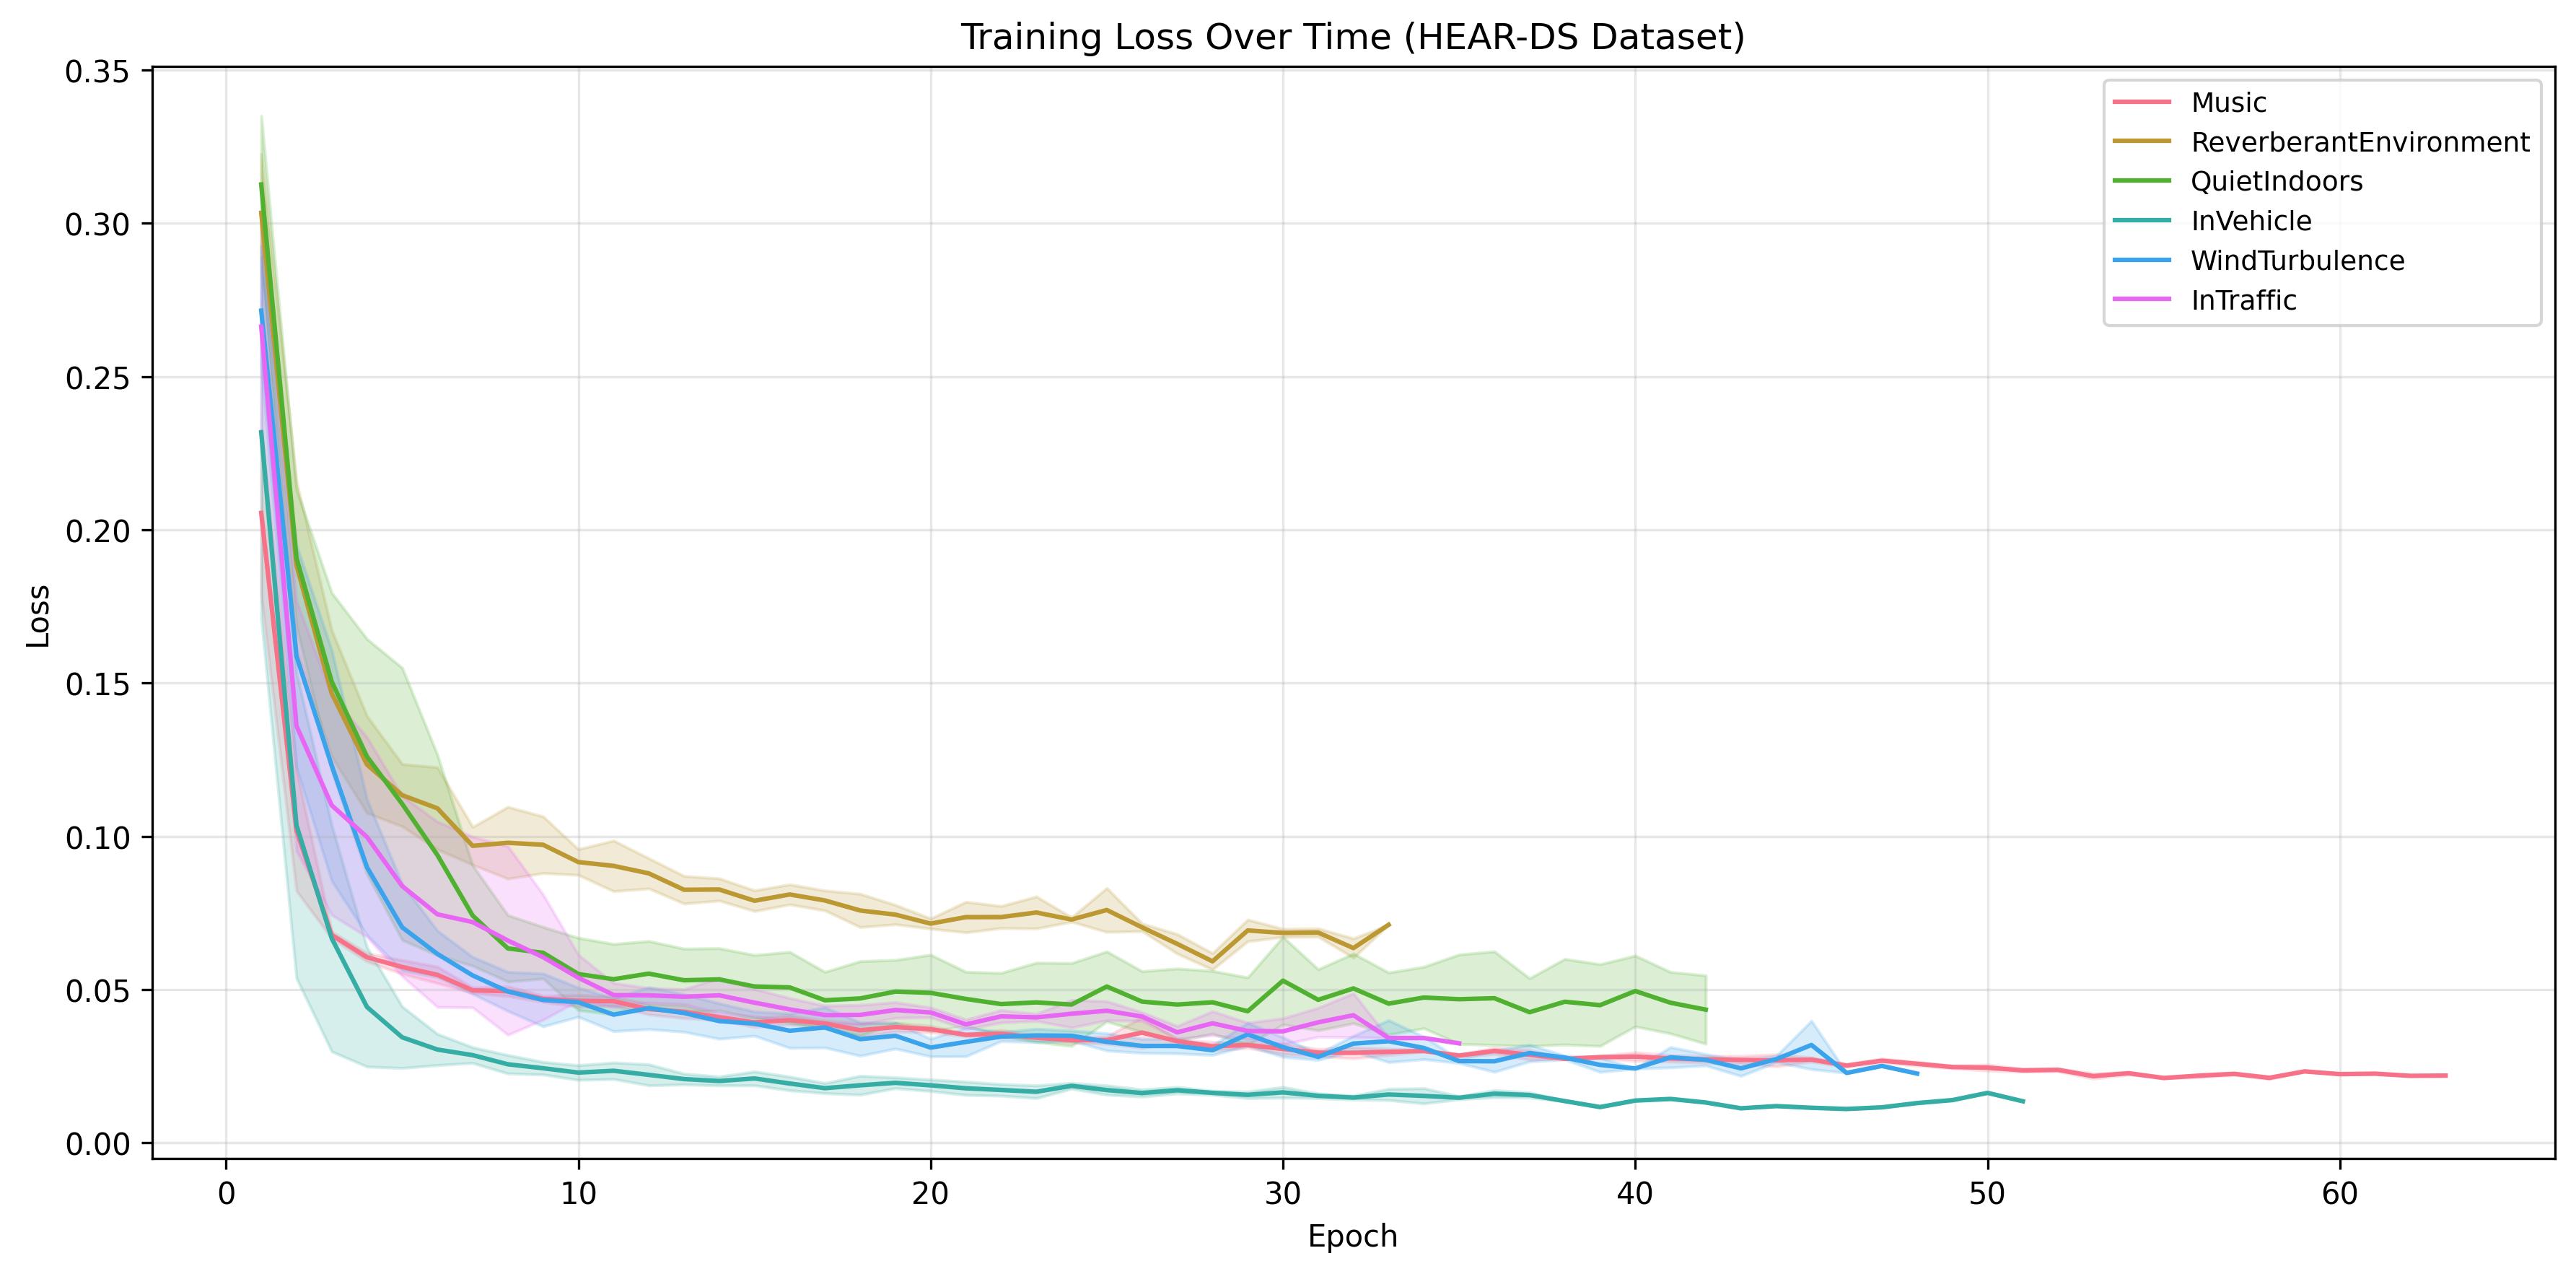
\includegraphics[width=0.9\textwidth]{se-hear-ds_training_losses.png}
   \caption{The training curves for the 6 SE models.}
   \label{fig:hear-ds-training-curves}
\end{figure}

In terms of how the model performs, we look at the STOI and PESQ scores at each SNR level.
Table \ref{tab:hear-ds-baseline} shows the baseline (unprocessed) average STOI and PESQ scores for different environments at various SNR levels.
Then after processing the speech signal, we get the results shown in Table \ref{tab:hear-ds-processed}.
Some interesting observations can be made from the table. Firstly, the model 
seems to perform better at lower SNR levels, i.e. 
the difference in increase in STOI and PESQ scores is higher at lower SNR levels.
This is a good sign as this is arguably the most challenging scenario 
as the speech signal is more difficult to understand since the background noise 
is more dominant. Secondly, there is a higher proportional increase in the STOI 
scores compared to PESQ scores. This suggests that the model is able 
to remove more of the noise, but perhaps at the cost of speech distortion. 
This is an important factor to consider and is certainly something we 
will be investigate in future work and which we elaborate more in Section \ref{sec:future-work}.
Just to show an indication of the speech separation, Figures \ref{fig:rev-spec}, \ref{fig:wind-spec}, \ref{fig:music-spec} and \ref{fig:in-vehicle-spec}
show the spectrograms of the clean, noisy, and enhanced speech signals for a selection of environments.
Although the enhanced signals demonstrate significant noise reduction, residual noise is 
observable in the initial and final segments. However, these initial results 
represent a promising start in prioritising speech over noise.
.
% As can be seen, it is quite evident that the background noise is removed, though there's evidence 
% of some signals being left over in the enhanced speech signal (especially visibile in the starting and ending segments).
% But it is a great start to see that the model is able to remove the noise to some extent.
\begin{table}[h]
    \begin{subtable}{\textwidth}
    \centering
    \begin{tabular}{l|ccccc|ccccc}
       \toprule
       Environment & \multicolumn{5}{c|}{STOI} & \multicolumn{5}{c}{PESQ} \\
       \cmidrule(lr){2-6} \cmidrule(lr){7-11}
       SNR (dB) & -10 & -5 & 0 & 5 & 10 & -10 & -5 & 0 & 5 & 10 \\
       \midrule
       Music & \small{0.25} & \small{0.37} & \small{0.49} & \small{0.61} & \small{0.71} & \small{1.07} & \small{1.06} & \small{1.09} & \small{1.14} & \small{1.29} \\
       WindTurbulence & \small{0.55} & \small{0.65} & \small{0.75} & \small{0.84} & \small{0.91} & \small{1.07} & \small{1.13} & \small{1.27} & \small{1.53} & \small{1.95} \\
       InTraffic & \small{0.21} & \small{0.35} & \small{0.50} & \small{0.64} & \small{0.77} & \small{1.12} & \small{1.05} & \small{1.08} & \small{1.16} & \small{1.36} \\
       InVehicle & \small{0.62} & \small{0.73} & \small{0.84} & \small{0.92} & \small{0.96} & \small{1.10} & \small{1.21} & \small{1.44} & \small{1.84} & \small{2.36} \\
       QuietIndoors & \small{0.30} & \small{0.43} & \small{0.58} & \small{0.71} & \small{0.82} & \small{1.03} & \small{1.05} & \small{1.08} & \small{1.17} & \small{1.38} \\
       ReverberantEnvironment & \small{0.22} & \small{0.35} & \small{0.49} & \small{0.63} & \small{0.77} & \small{1.17} & \small{1.08} & \small{1.12} & \small{1.23} & \small{1.47} \\
       \bottomrule
    \end{tabular}
    \caption{Baseline (unprocessed) STOI and PESQ scores for different environments at various SNR levels.}
    \label{tab:hear-ds-baseline}
    \end{subtable}
    \begin{subtable}{\textwidth}
    \centering
    \begin{tabular}{l|ccccc|ccccc}
       \toprule
       Environment & \multicolumn{5}{c|}{STOI} & \multicolumn{5}{c}{PESQ} \\
       \cmidrule(lr){2-6} \cmidrule(lr){7-11}
       SNR (dB) & -10 & -5 & 0 & 5 & 10 & -10 & -5 & 0 & 5 & 10 \\
       \midrule
       Music & \small{0.42} & \small{0.57} & \small{0.69} & \small{0.77} & \small{0.83} & \small{1.11} & \small{1.18} & \small{1.30} & \small{1.46} & \small{1.67} \\
       WindTurbulence & \small{0.62} & \small{0.72} & \small{0.79} & \small{0.85} & \small{0.89} & \small{1.18} & \small{1.29} & \small{1.44} & \small{1.61} & \small{1.77} \\
       InTraffic & \small{0.34} & \small{0.51} & \small{0.64} & \small{0.74} & \small{0.82} & \small{1.08} & \small{1.15} & \small{1.25} & \small{1.40} & \small{1.57} \\
       InVehicle & \small{0.73} & \small{0.82} & \small{0.88} & \small{0.92} & \small{0.95} & \small{1.34} & \small{1.54} & \small{1.78} & \small{2.02} & \small{2.25} \\
       QuietIndoors & \small{0.39} & \small{0.56} & \small{0.68} & \small{0.77} & \small{0.83} & \small{1.09} & \small{1.16} & \small{1.27} & \small{1.46} & \small{1.65} \\
       ReverberantEnvironment & \small{0.28} & \small{0.43} & \small{0.58} & \small{0.71} & \small{0.80} & \small{1.08} & \small{1.10} & \small{1.17} & \small{1.29} & \small{1.38} \\
       \bottomrule
    \end{tabular}
    \caption{Processed STOI and PESQ scores for different environments at various SNR levels.}
    \label{tab:hear-ds-processed}
    \end{subtable}
    \caption{}
\end{table}

\FloatBarrier
\begin{figure}[h]
    \caption{Selected spectrograms of the clean, noisy and enhanced speech signals}
    \centering
    \hspace{0pt}%
    \begin{subfigure}{0.42\textwidth}
        \centering
        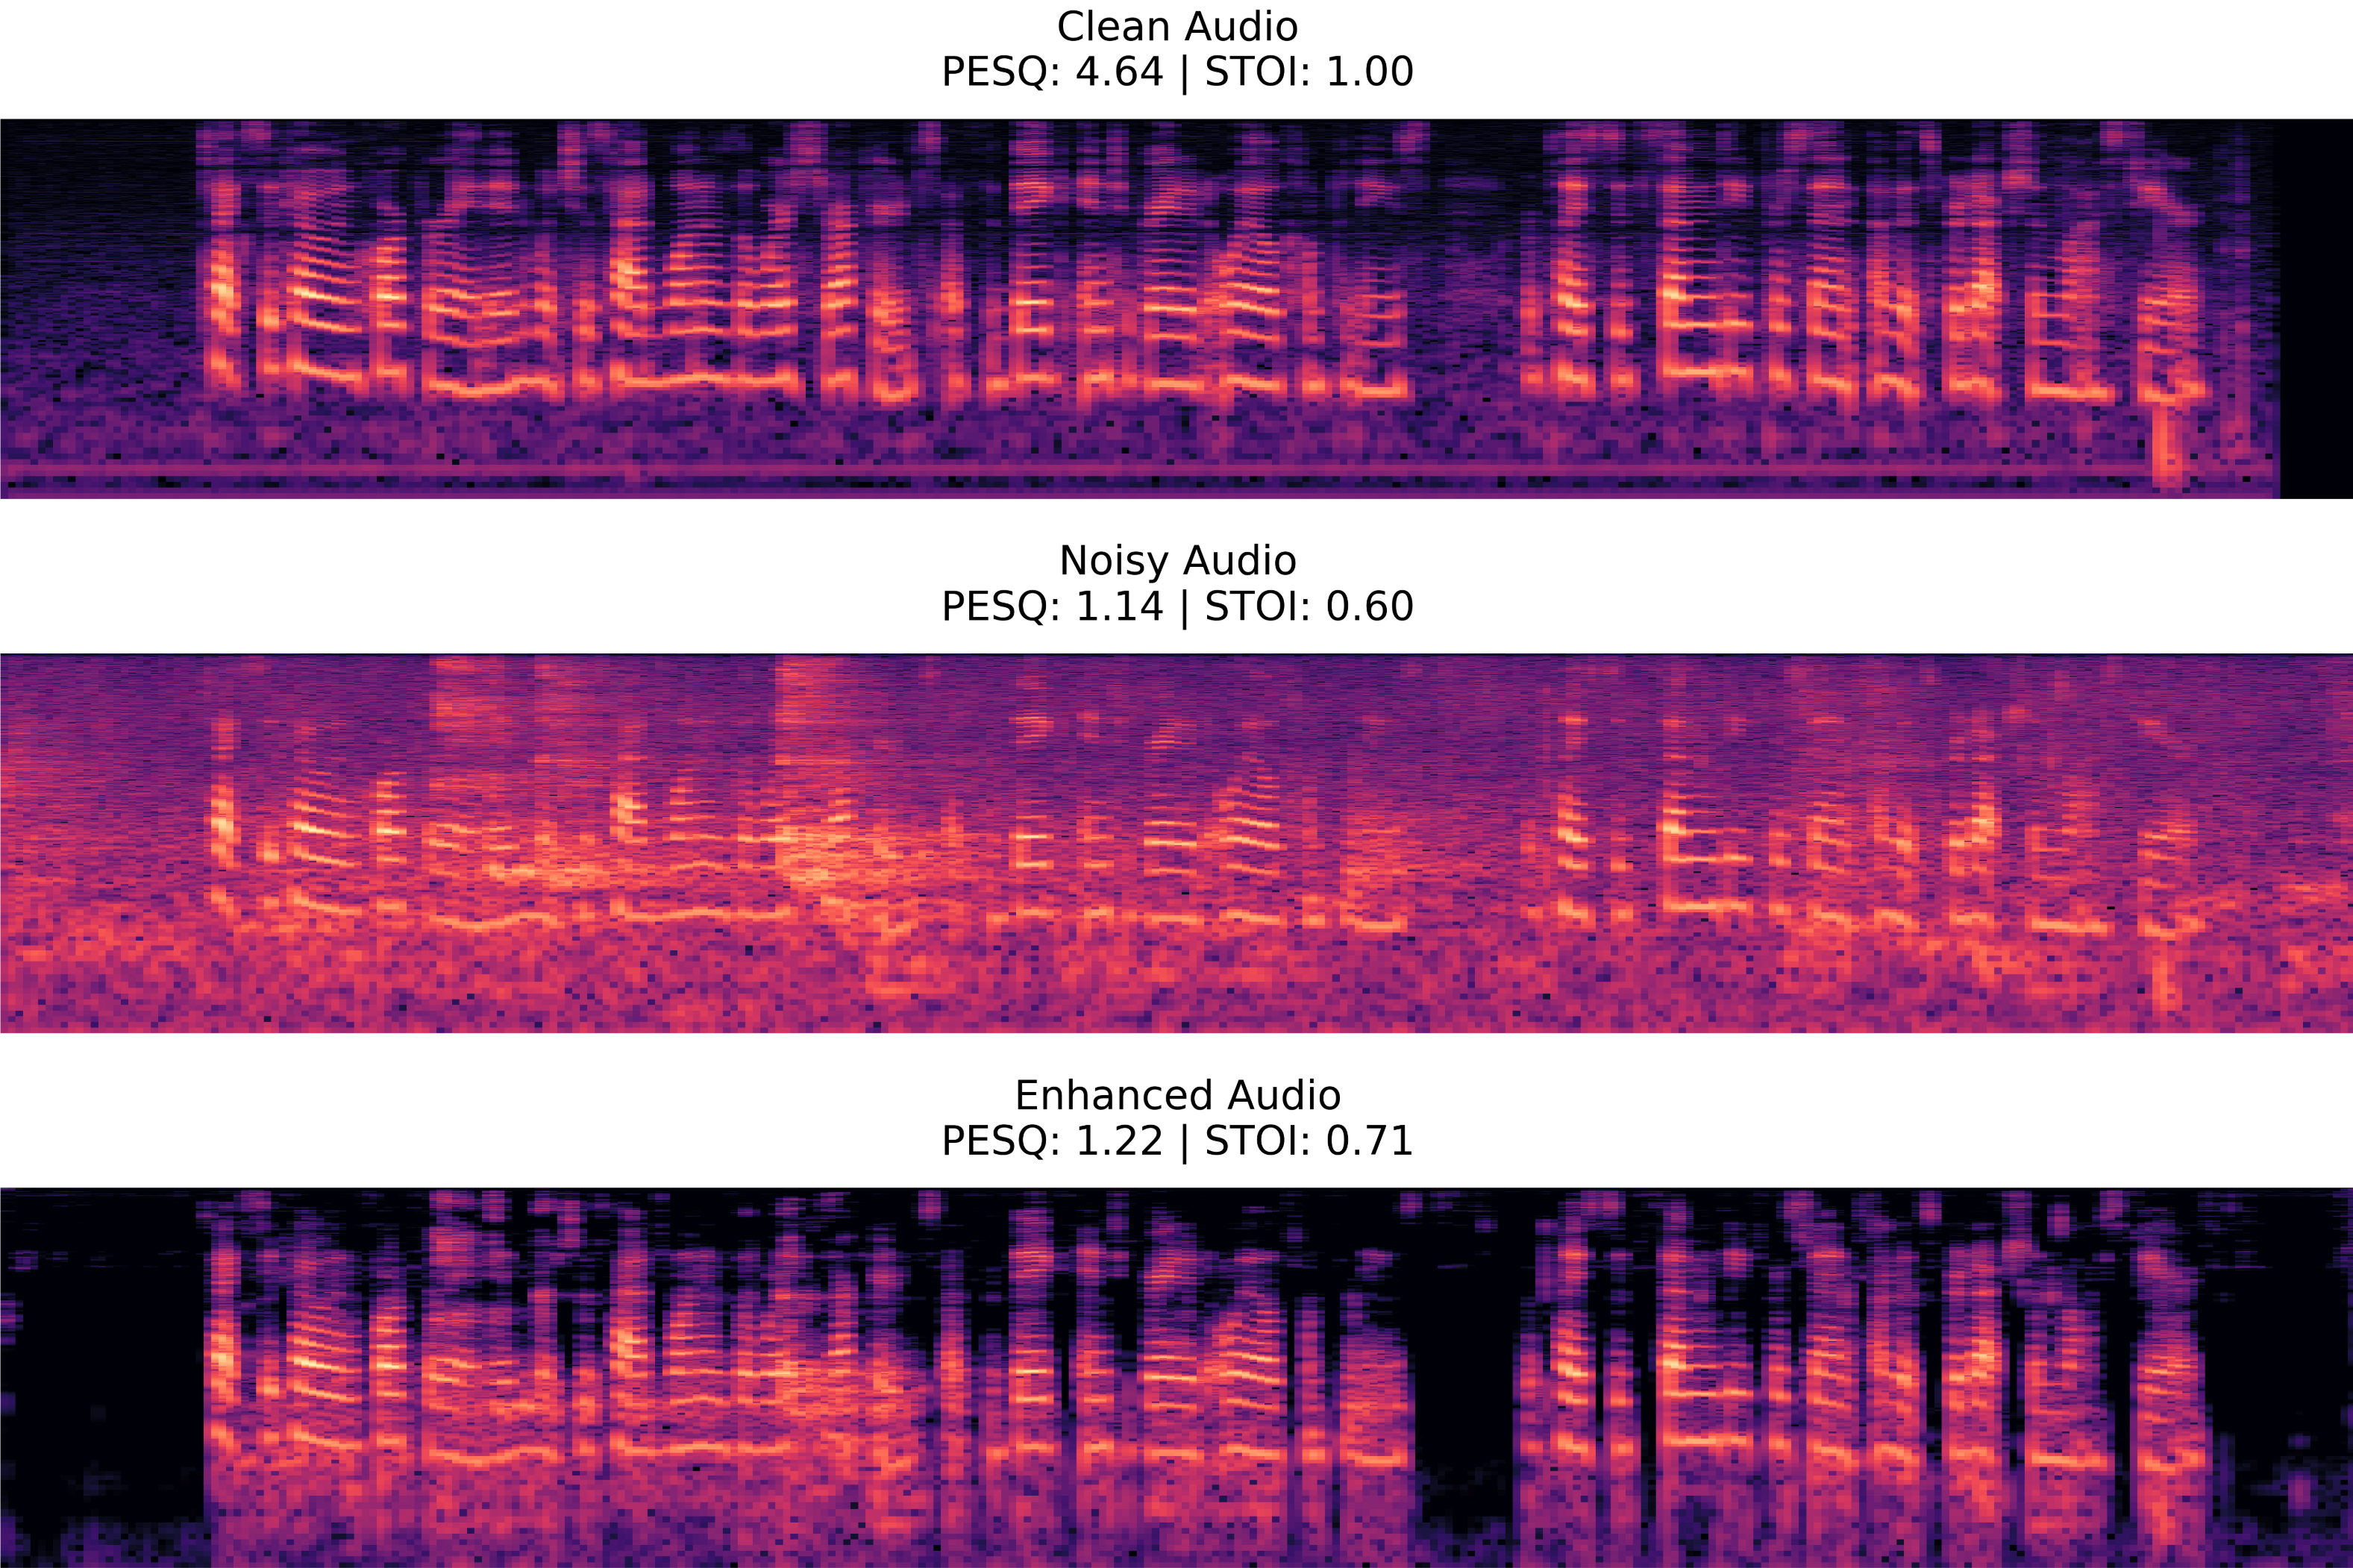
\includegraphics[width=\textwidth]{rev-spec.png}
        \caption{In a Reverberant Environment}
        \label{fig:rev-spec}
    \end{subfigure}%
    \hspace{0.02\textwidth}%
    \begin{subfigure}{0.42\textwidth}
        \centering
        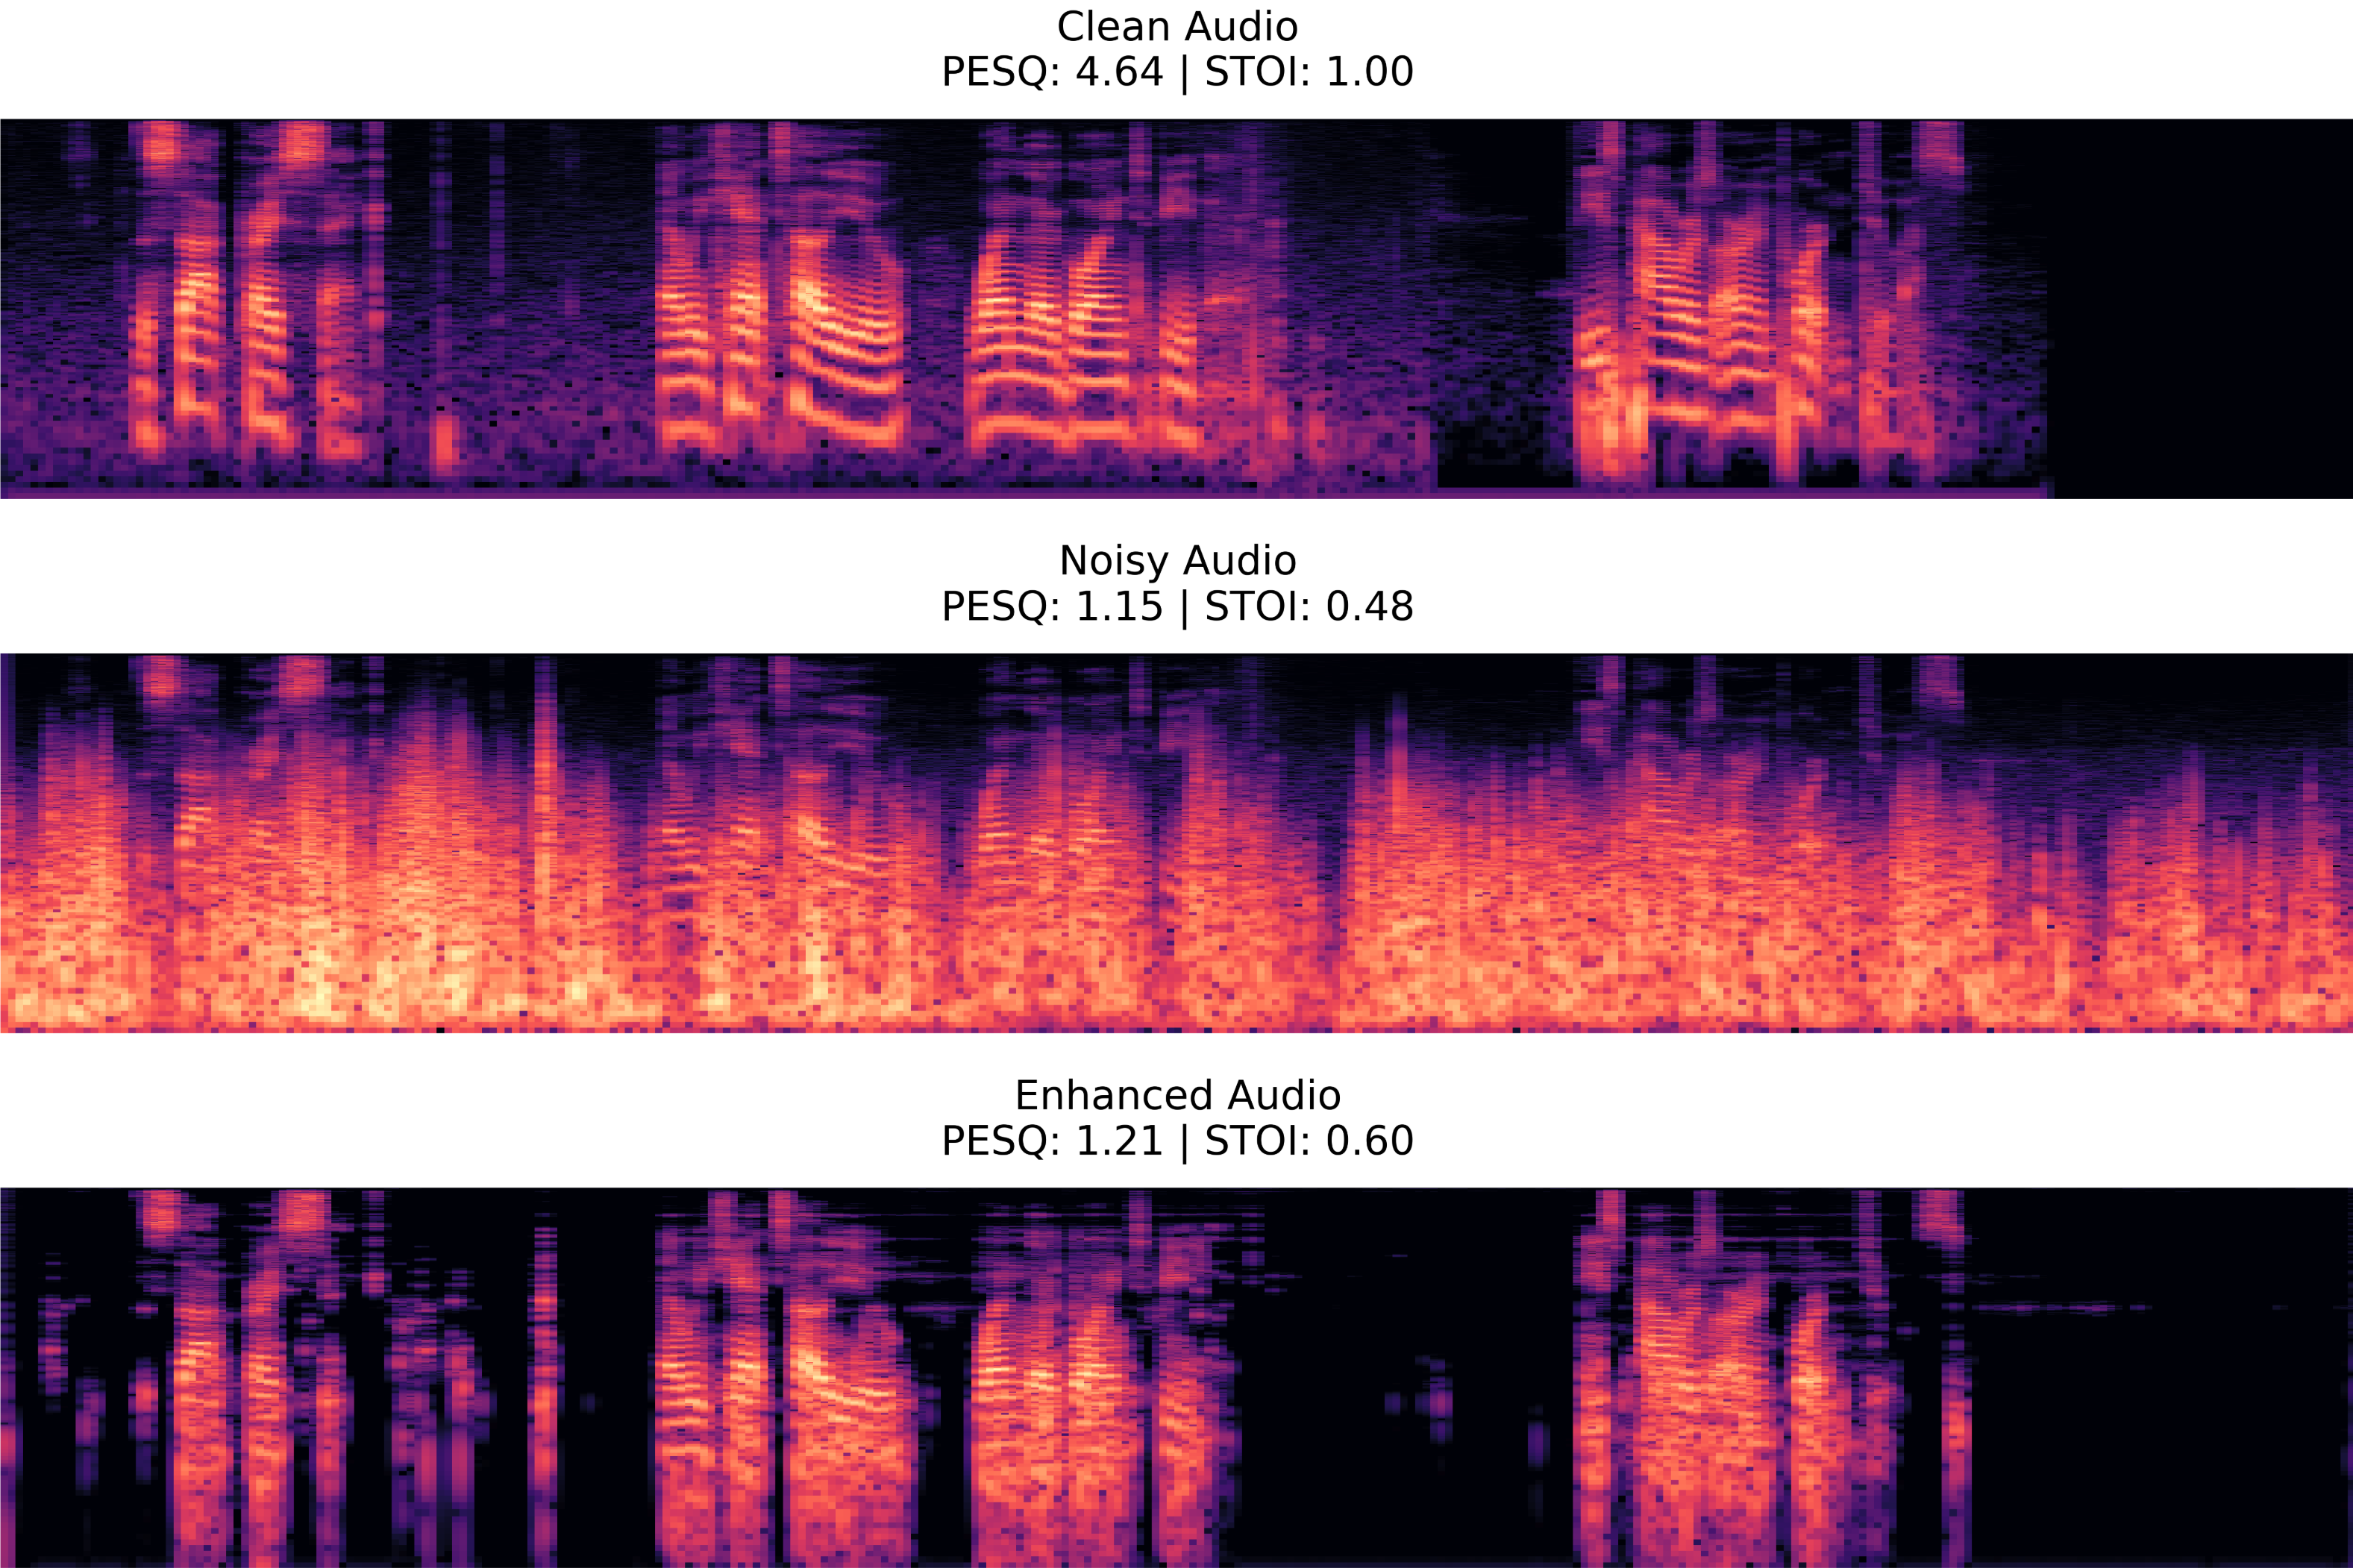
\includegraphics[width=\textwidth]{wind-spec.png}
        \caption{With Wind Turbulence}
        \label{fig:wind-spec}
    \end{subfigure}
    \begin{subfigure}{0.42\textwidth}
        \centering
        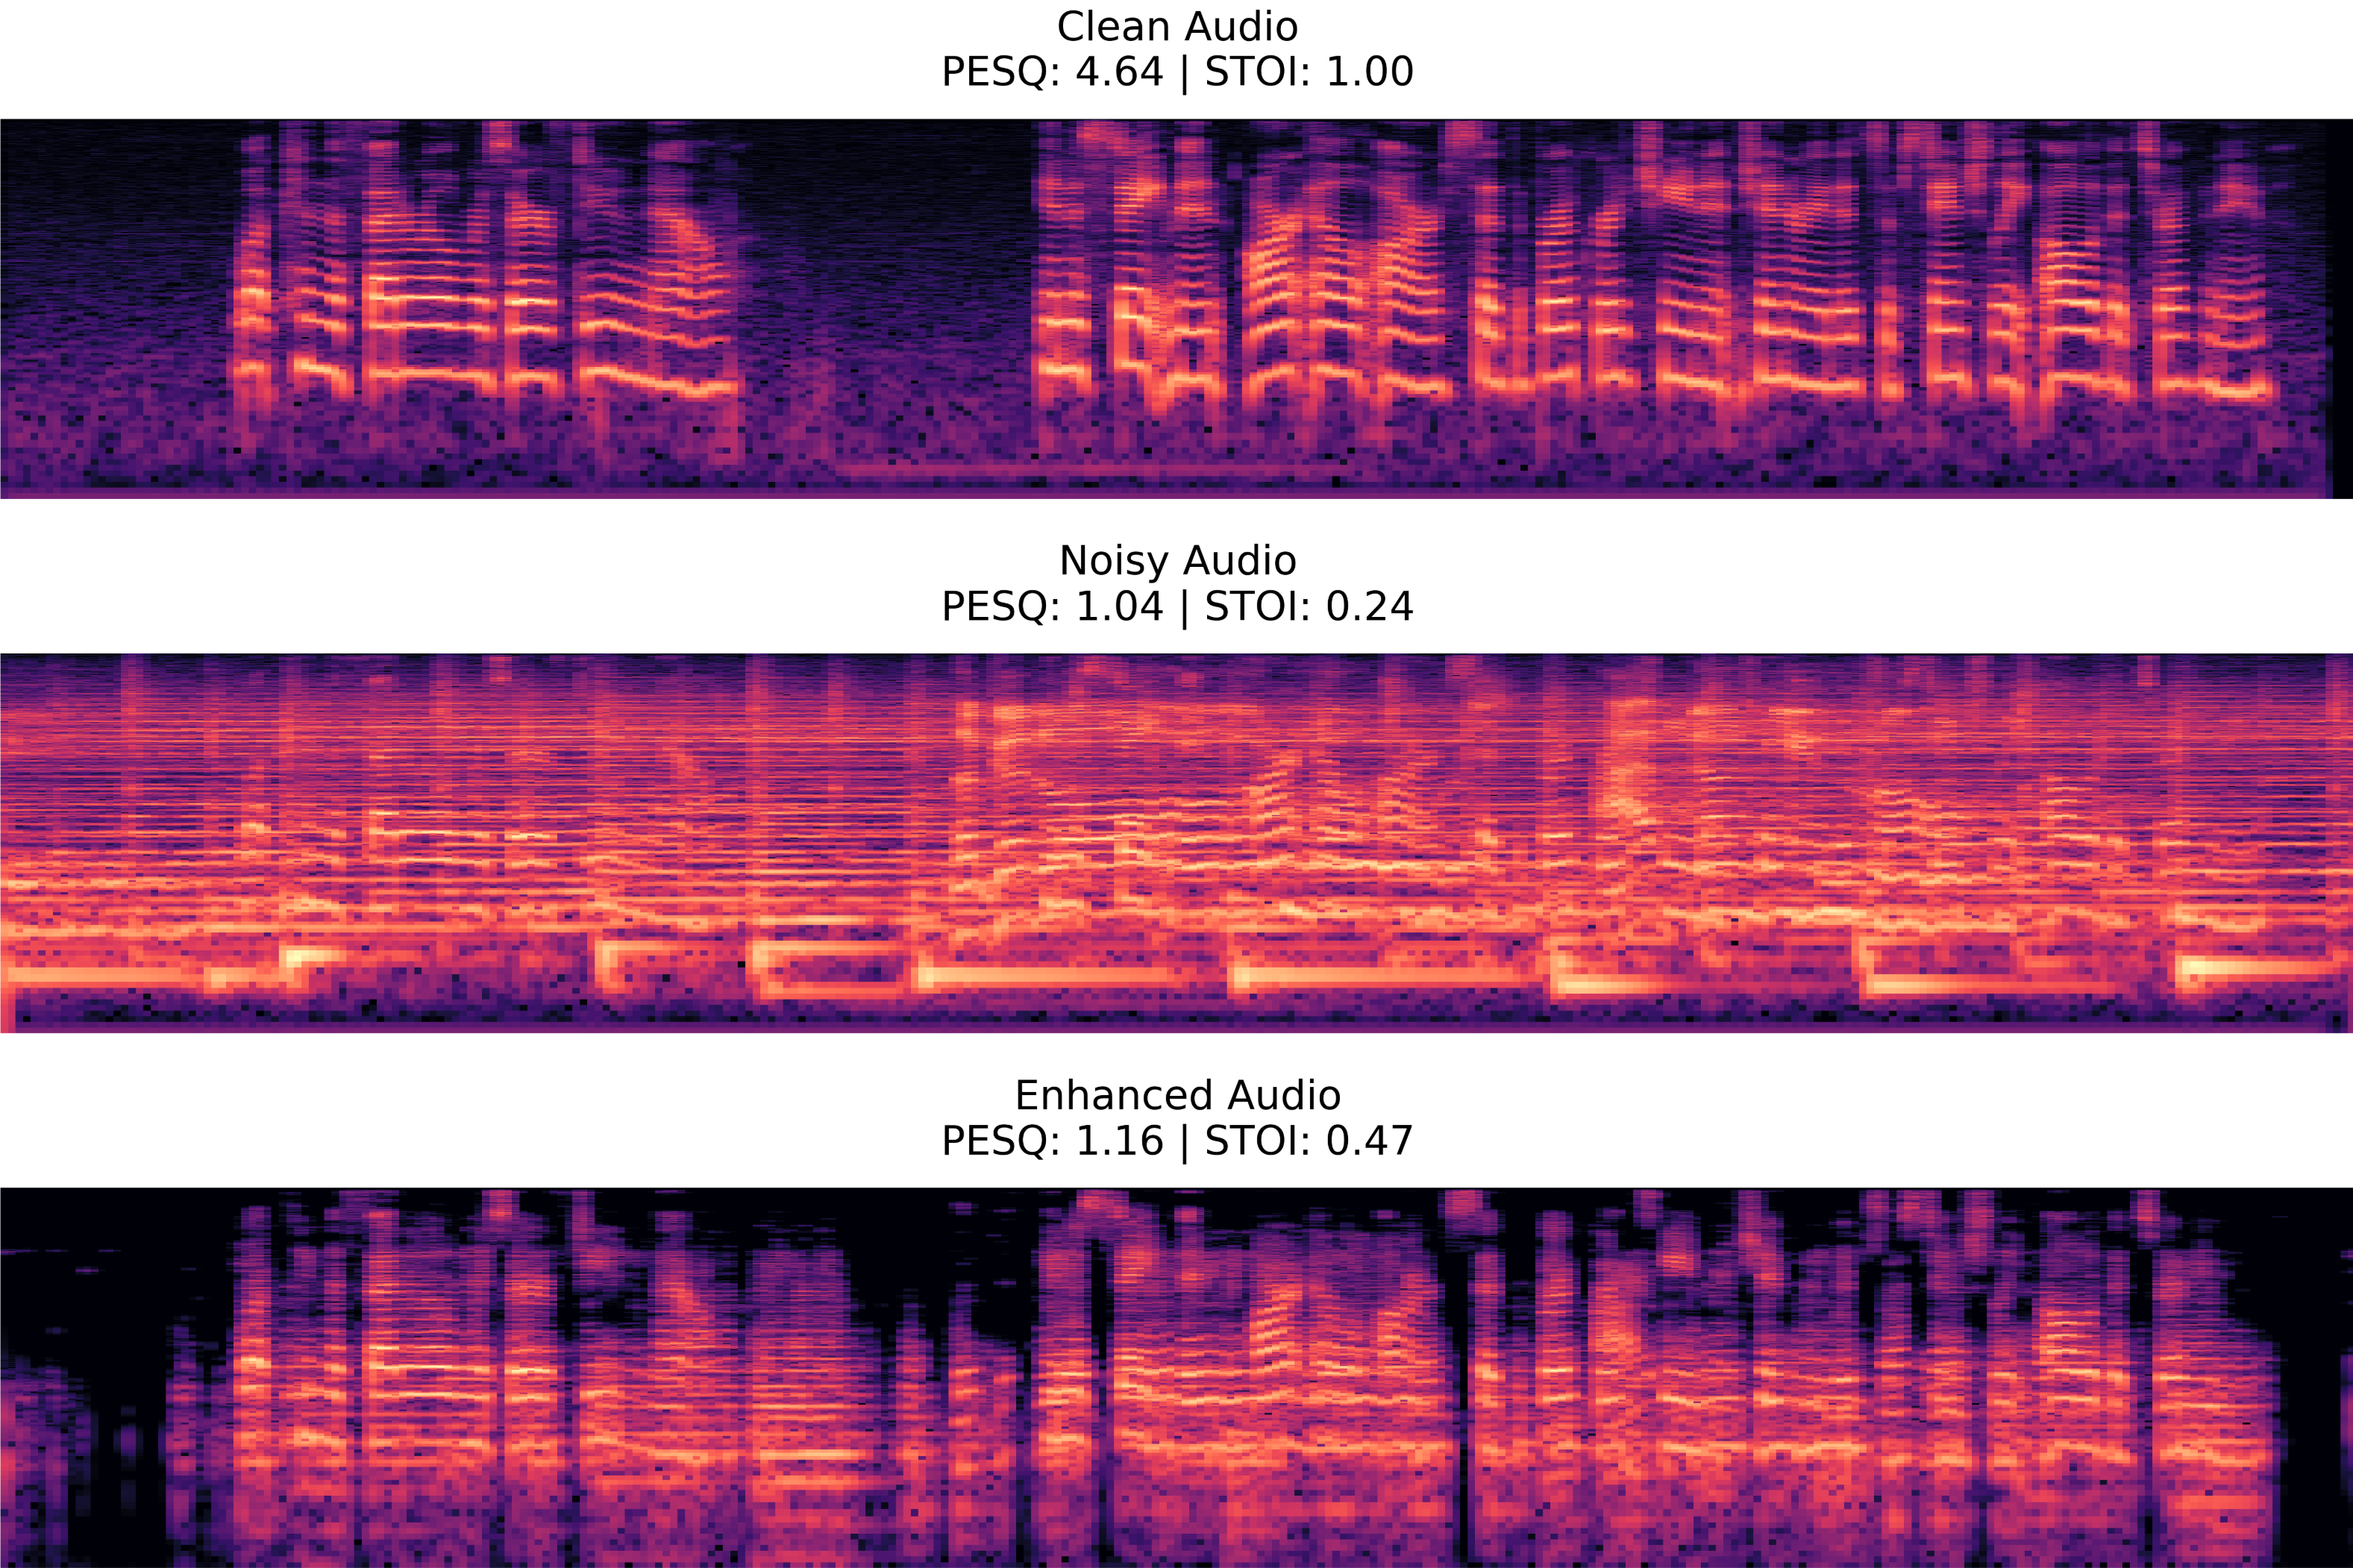
\includegraphics[width=\textwidth]{music-spec.png}
        \caption{With Music}
        \label{fig:music-spec}
    \end{subfigure}%
    \hspace{0.02\textwidth}%
    \begin{subfigure}{0.42\textwidth}
        \centering
        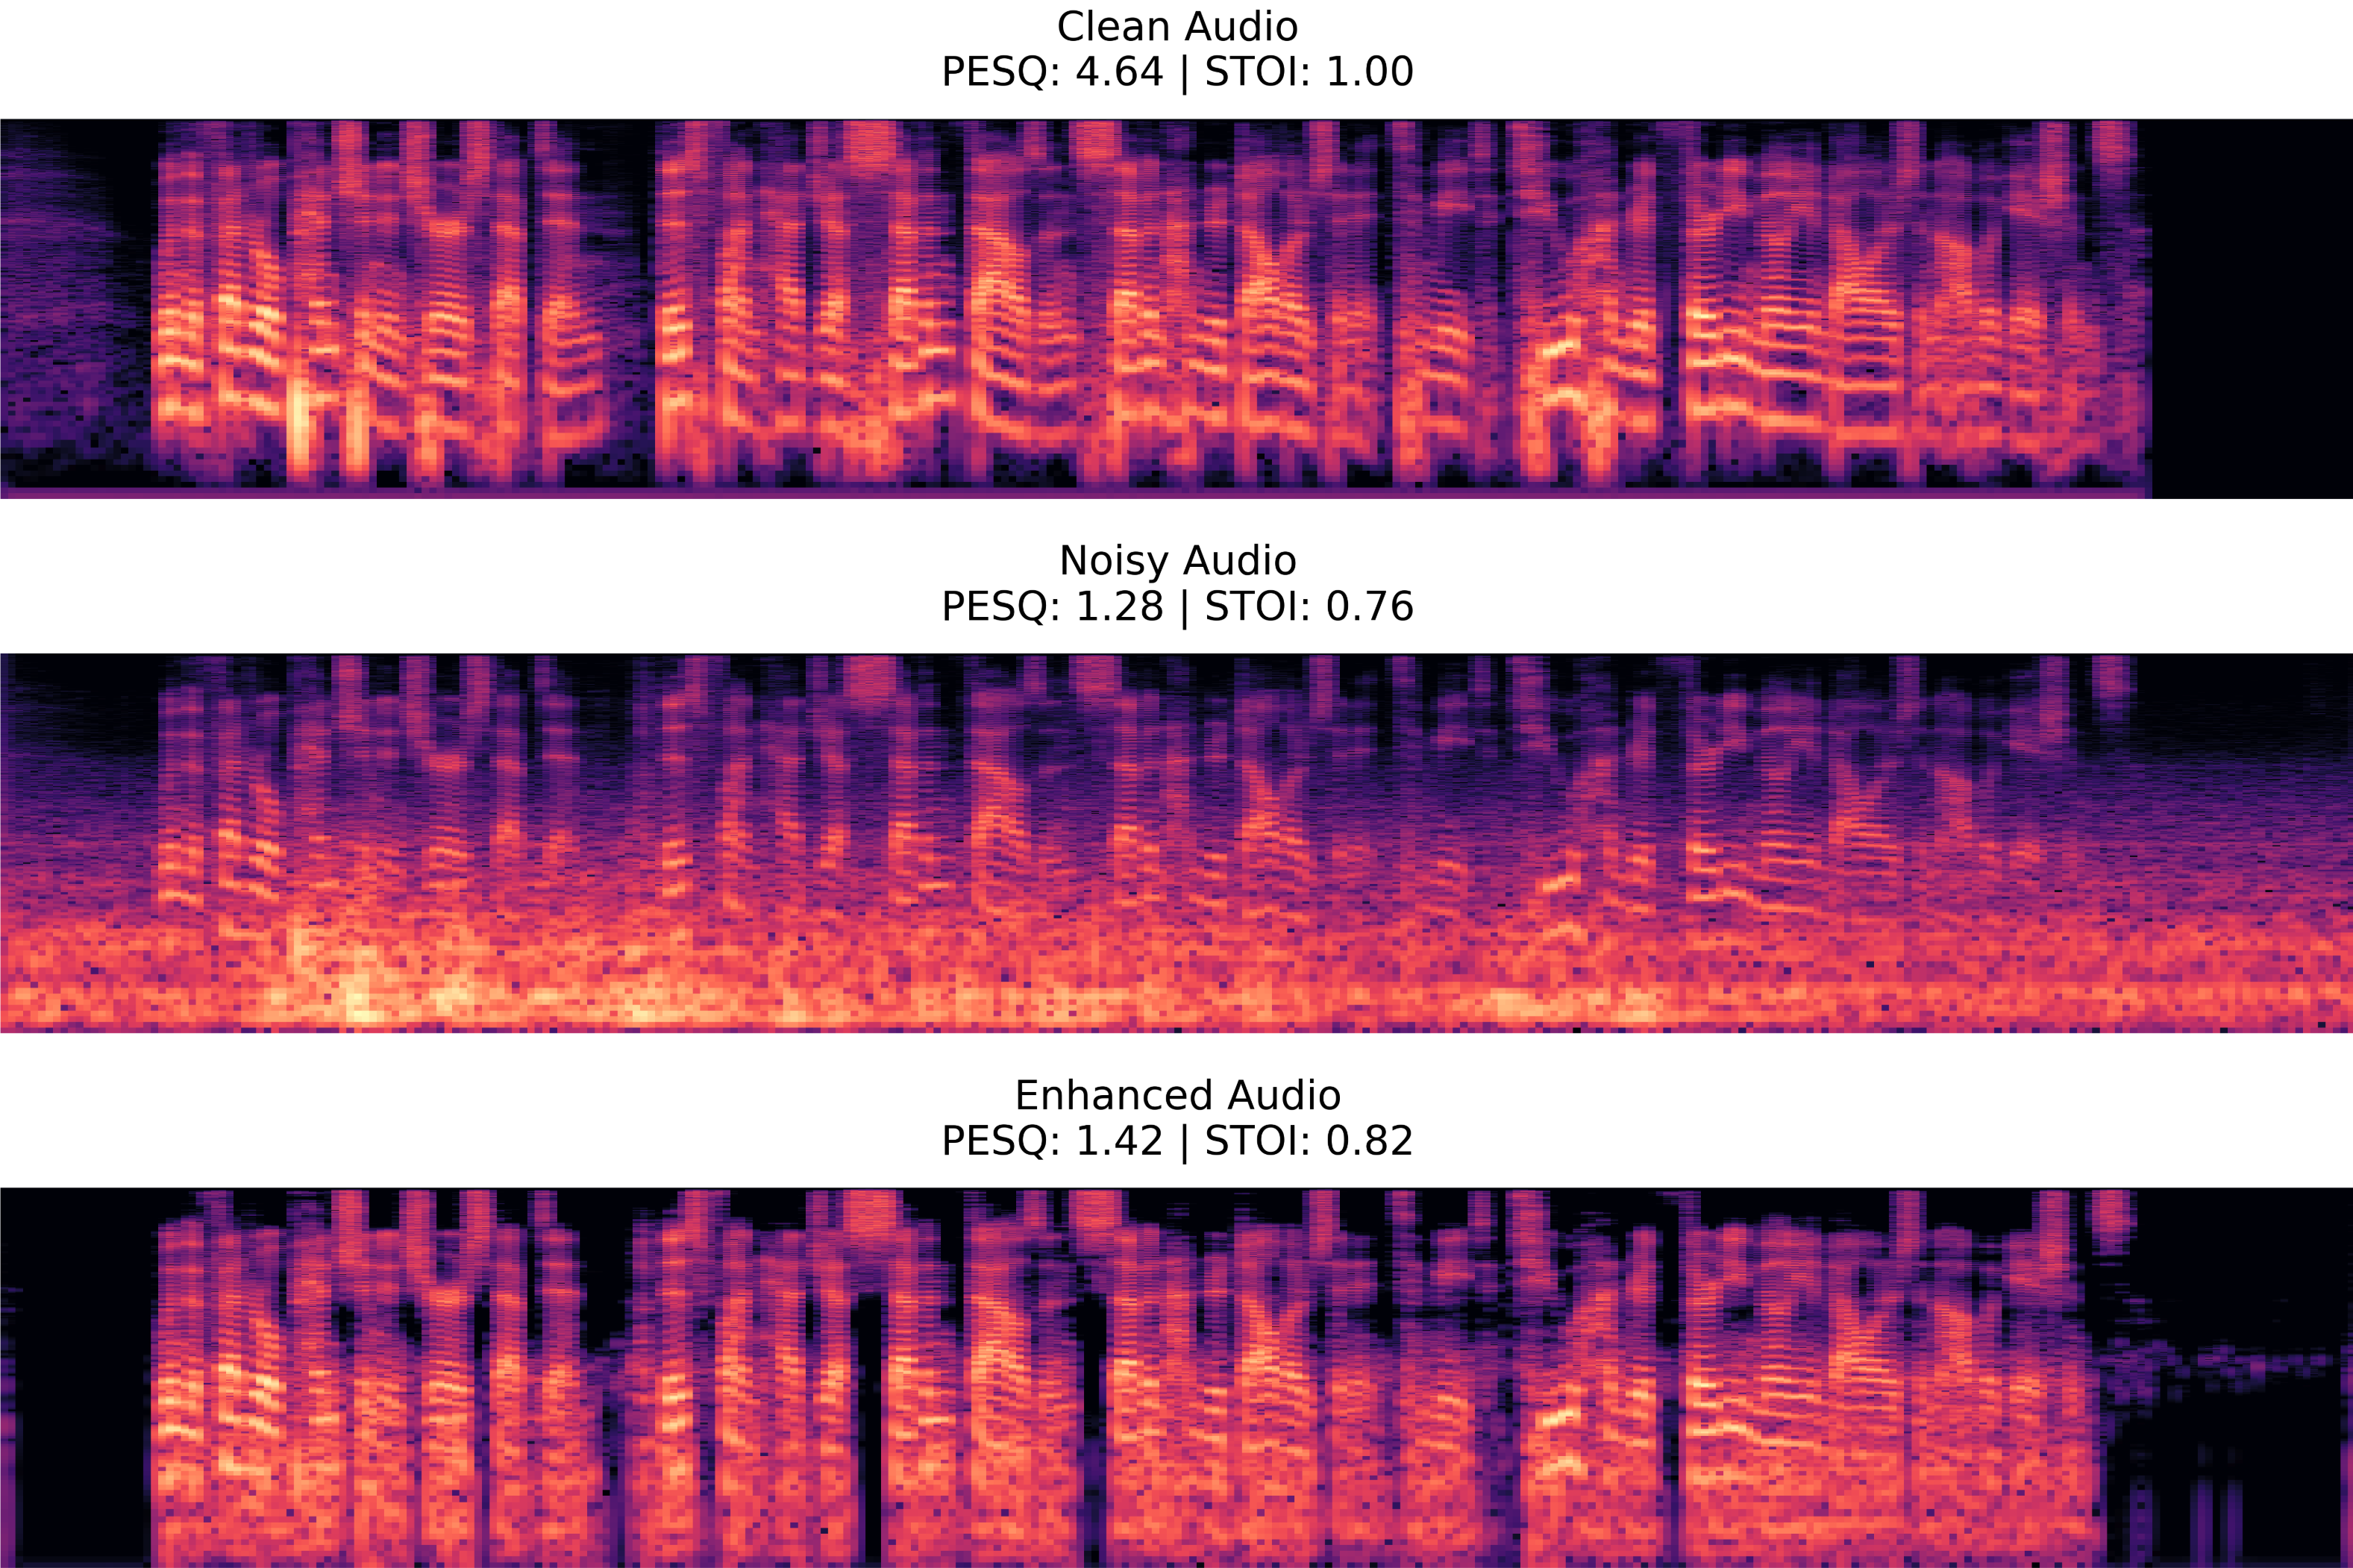
\includegraphics[width=\textwidth]{in-vehicle-spec.png}
        \caption{In Vehicle Environment}
        \label{fig:in-vehicle-spec}
    \end{subfigure}
\end{figure}
\FloatBarrier



\section{Validating against VOICEBANK + DEMAND}
In order to validate the implementation of the proposed model, we compare the results 
with the work by \citet{kim_specmix_2021} who proposed the SpecMix technique. 
Although a direct comparison with the original CED model reported by \citet{tan18_interspeech} 
would have been ideal, practical constraints — notably the extensive dataset requirements 
(exceeding 500\,h of data) and the reproducibility challenges discussed in Section \ref{sec:criticism} — 
required an alternative comparison. Consequently, the evaluation was performed against the work 
introducing the SpecMix technique, which has been applied to a range of audio-related 
tasks, including speech enhancement \citep{kim_specmix_2021}. Consistent with the study 
by \citet{kim_specmix_2021}, the \vbd dataset was employed for experimental 
validation. The paper itself is compared with other techniques including Mixup \citep{zhang_mixup_2017},
CutMix \citep{yun_cutmix_2019} and SpecAugment \citep{park_specaugment_2019}. In terms 
of the model that \citet{kim_specmix_2021} used, for the SE task, they 
took inspiration from the U-Net architecture \citep{ronneberger_unet_2015}.
It has similarities to the CED model that is employed in this dissertation 
since it also uses an encoder-decoder architecture. But the main difference 
lies in its final layer, which is another neural network called the 
'Phase Sensitive Mask'. Suffice to say, the complexity of the model 
is likely higher than the CED model so we should expect the model 
to perform better.

\begin{figure}[h]
   \centering
   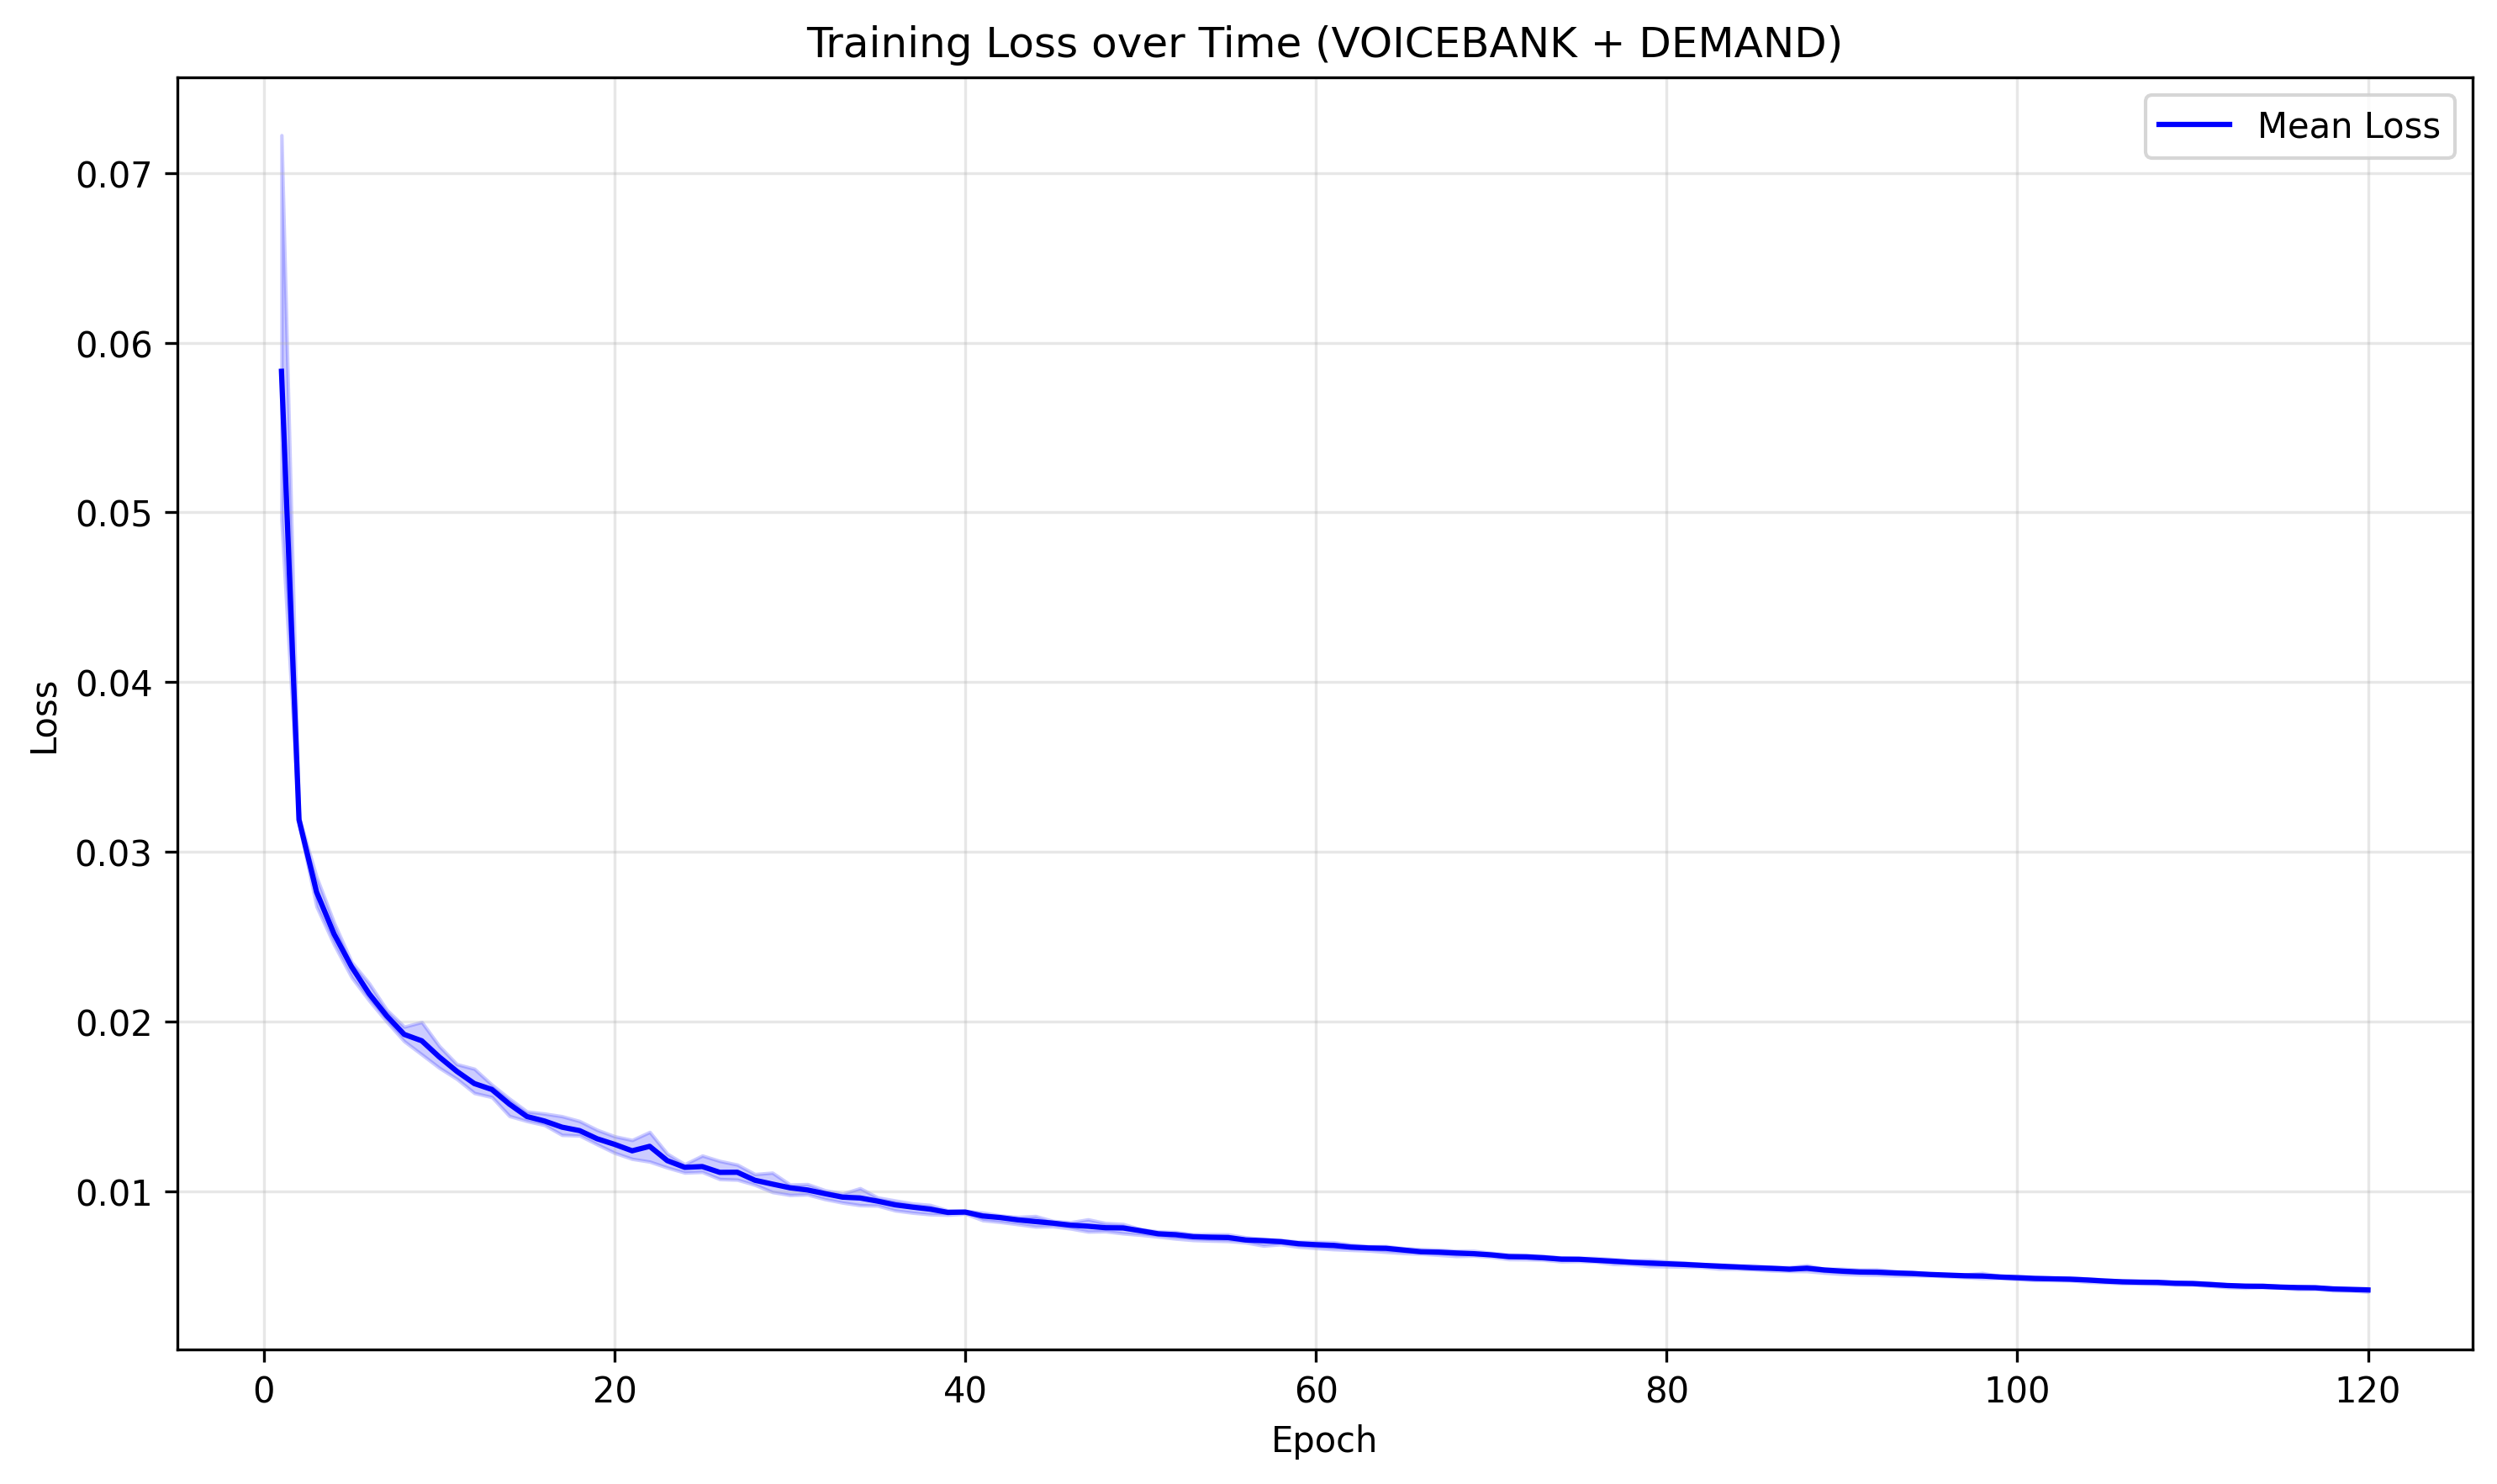
\includegraphics[width=0.9\textwidth]{se-VOICEBANK-training-losses.png}
   \caption{The training curves for the SE model on the \vbd dataset.}
   \label{fig:se-voicebank-training-losses}
\end{figure}
As a dataset already contains the noisy and clean speech signals, we do not 
have the luxury of having control over the SNR levels, which as a 
consequence means that  we cannot analyse the performance of the model at different 
SNR levels. However given that this is a validation of the model's implementation, 
we can at least compare the results against the paper which proposed the SpecMix technique.
Additionally, the dataset is split into a training and a test set, so 
manual splitting was not required here. 
After training the model five times, we get the resulting training curve shown in Figure \ref{fig:se-voicebank-training-losses}.
No early stopping was applied here, so the model was trained for 120 epochs which was the maximum number of epochs set however,
by observing the training curves, we can see that the model has converged by then. 

After testing the model in the test set, we get the results shown in Table \ref{tab:voice_enhancement_metrics}.
\citet{kim_specmix_2021} did not report the STOI metric, so we only compare the PESQ scores.
But, as we can see, the model is just about on par with the reported results from the paper.
This is a reassuring sign that not only the model's implementation is correct, but also
that the model is able to generalise to a new dataset. For future work, it would 
be interesting to see if employing the techniques mentioned and proposed by \citet{kim_specmix_2021}
would improve the performance of the model when using the CED model. 


\begin{table}[h]
   \centering
   \begin{tabular}{l|cc}                                                                               
   \toprule
   Condition & STOI & PESQ \\
   \midrule
   Noisy (Unenhanced) & 0.79 & 2.01 \\   
   SpecMix No Augmentation \citep{kim_specmix_2021} & - & 2.5 \\
   SpecMix \citep{kim_specmix_2021} & - & 2.54 \\
   Mixup \citep{zhang_mixup_2017} & - & 2.50 \\
   CutMix \citep{yun_cutmix_2019} & - & 2.52 \\
   SpecAugment \citep{park_specaugment_2019} & - & 2.41 \\
   \textbf{Our method (CED)} & 0.82 & 2.44 \\
   \bottomrule
   \end{tabular}
   \caption{Average STOI and PESQ scores for noisy and enhanced speech. Mixup, CutMix and SpecAugment results are taken 
   from \citet{kim_specmix_2021}.}
   \label{tab:voice_enhancement_metrics}
\end{table} 
\section{Feasibility}
\begin{table}[h]
   \centering
   \begin{tabular}{lccc}
      \toprule
      Model & FLOP(s) Count & Parameters & Theoretical Inference Time\footnotemark \\
      \midrule
      CED (10s) & 25.244G & 17.579M & 3.278 seconds \\ % 3.2784415584 seconds
      CED* (1s) & 2.524G & 1.758M & 327ms \\ % 0.3277922078
      CED* (5s) & 12.622G & 8.790M & 1.639 seconds \\ % 1.6392207792
      \bottomrule
   \end{tabular}
   \caption{FLOPs and parameters of the CED model for different time segments.}
   \label{tab:ced-model-metrics}
\end{table}
To evaluate the SE task from a hardware perspective, we look at the FLOPs and parameters of the CED model.
Table \ref{tab:ced-model-metrics} presents the FLOPs and parameter counts for 10 second samples, 
indicating a much higher complexity than the ASA task. Although the model was trained on 10s samples 
as mentioned in the beginning of this chapter, it is worth investigating the performance of the model 
on shorter time segments. Accordingly, estimates for 1s and 5s samples are also provided, albeit 
provisionally, since the STFT parameters have not been validated for these durations. Nevertheless,
these theoretical inference times are outside the acceptable latency for HAs so future work at 
the first stage would be to reduce the FLOPs of the model of which we discuss more in Section \ref{sec:future-work}.
\footnotetext{{Assumes a 7,700M FLOPs capable device and that the formula in \ref{eq:inference-time} is used.}}
% Benchmarking CRNN on cpu...
% --- thop results ---
% [INFO] Register count_convNd() for <class 'torch.nn.modules.conv.Conv2d'>.
% [INFO] Register count_normalization() for <class 'torch.nn.modules.batchnorm.BatchNorm2d'>.
% [INFO] Register count_lstm() for <class 'torch.nn.modules.rnn.LSTM'>.
% [INFO] Register count_convNd() for <class 'torch.nn.modules.conv.ConvTranspose2d'>.
% FLOPs: 25.244G, Parameters: 17.579M

% --- Inference time measurement ---
% Average inference time: 502.79 ms (±67.39 ms)
% Operations per second: 50.21 GOPS
% Operations per parameter: 2856.02

% ==================================================
% MODEL METRICS
% ==================================================

% PARAMETER COUNTS:
%   Total Parameters:      17,579,459.0

% INFERENCE PERFORMANCE:
%   Avg Inference Time:    502.79 ms
%   Std Inference Time:    67.39 ms
%   FLOPs per Inference:   25,243,615,716.0
%   Operations per Second: 50.21 GOPS
%   OPS per Parameter:     2856.02

% ==================================================


\chapter{Conclusions}
\label{chap:conclusions}
\section{Review}
In this part of the dissertation we explore the novel datatset \heards by \citet{Huwel2020HearDS}.
The very first hypothesis was to see if the ASA model shown by \citet{Huwel2020HearDS} 
could be reproduced. We were not able to fully reproduce the accuracies that the paper 
reports, and we attribute this to a small deviation
in the speech mixing dataset, and the omission of 
the HRTF during speech mixing in the paper. We also 
extended the analysis of the model's performance 
by considering precision, recall and F1 scores 
due to the inherent imbalance in the dataset.

Secondly, we hypothesised that the ASA model 
would be able to generalise and be trained 
faster if utterance-level data augmentation were utilised. 
While the training times were reduced, the performance 
of the model was found to be slightly worse. 

Third, we decided to see if the claim by \citet{Huwel2020HearDS} 
that the use of the Adam optimiser was not suited 
for the ASA task was valid. We found that the model 
trained using the Adam optimiser received 
comparable results to the model trained using the 
SGD optimiser, and at a slightly faster convergence.

As a means of validation, and the doubt raised 
by the higher accuracies in our results compared 
to the paper by \citet{Huwel2020HearDS}, we 
performed a validation of the model's implementation
against the work by \citet{schindler_multi-temporal_2018} 
who used the TUT Acoustic Scenes 2016 dataset to 
train an ASA model. Through this validation, we 
found that the model's implementation is correct 
and that the model is also able to generalise to 
a new dataset, which is a good sign.

Lastly, on the ASA front, 
the feasibility hypothesis 
of the ASA model being used in a HA was 
evaluated. We did this by considering 
the state of the art HAs capability, and through that, 
it suggests that the ASA model is capable of being used 
in a HA.

To date, we have not found any publications on 
using the \heards dataset for the SE task, so we 
took it upon ourselves to create a SE model 
for the dataset. Inspired by \citet{katagiri_handbook_2000}'s
categorisation of SE models, we created a SE model that can 
be called a state dependent model. Our final hypothesis was 
that of pertaining of whether the SE model inspired 
by \citet{tan18_interspeech} would be able to 
generalise to the \heards dataset. This was found 
to be possible, but there is certainly room for improvement 
from a performance perspective. Due to the model's 
complexity, we validated the model's implementation 
against the work by \citet{kim_specmix_2021} who proposed 
the SpecMix technique. We found that the model is 
able to generalise to the \vbd dataset and that the 
performance seems comparable to the paper.

Lastly, the feasibility of the SE model being used 
in a HA was evaluated. This was found to be rejected 
with absolute certainty. The model's latency is too high and 
it is because of the high number of parameters and 
consequently high FLOPs required to process the 
signal in an acceptable manner for an HA user to not 
notice the delay.

\section{Future Work}
\label{sec:future-work}
This dissertation opens several promising avenues for future exploration.
First, the current SE model is not suitable for state-dependent deployment
in hearing aids. A potential solution is to develop a model trained on
shorter speech segments, possibly coupled with efforts to reduce the model
FLOP(s) count as suggested by \citet{liu_simple_2023}. In addition, refining
hyper-parameter settings or reconsidering the model architecture may be 
beneficial such as considering time domain/end-to-end models.

There is also an exciting area of research in 
the speech community to train neural models 
that take into account human preferences \citep{Zhang2024SpeechAlignAS}.
Moreover, Phonak's white paper further elucidates
this approach \citep{Hasemann2024PhonakSphere}.
These methods share similarities to the Generative Adversarial Network (GAN)  
as described in \citet{Bai2022PerceptualLoss}. 
In this context, \citet{Fu2018QualityNet} introduced 
QualityNet, an end-to-end network to estimate PESQ scores without a clean
reference. They then presented the applicability of the model to the SE task
to build a GAN based framework called MetricGAN.
Building on this, \citet{Bai2022PerceptualLoss} extended QualityNet
to also learn STOI, resulting in the PESQ-STOI-QualityNet (PSQN) framework.
It could be interesting to see if the SE model could be trained using 
this framework to improve the performance of the model.

On the topic of human preferences, 
the incorporation of a metric 
that takes into account HA's user's preferences
such as the Hearing-Aid Speech Perception Index (HASPI)
proposed by \citet{Kates2021HASPI} would be interesting.

Currently, the feasibility of the models is done by 
assuming that the latency of a model can be 
calculated by considering the FLOP(s) of the device 
benchmarking the model. It would be interesting to see 
if this actually holds on lower-powered devices 
such as a microcontroller or a Raspberry Pi.

Lastly, for reproducibility, mixing the \heards dataset 
with the \chime{2} dataset and the incorporation of 
a HRTF is something that could be investigated in the future.


\bibliography{mybibfile}


% You may delete everything from \appendix up to \end{document} if you don't need it.
% \appendix

% \chapter{First appendix}

% \section{First section}

% Any appendices, including any required ethics information, should be included
% after the references.

% Markers do not have to consider appendices. Make sure that your contributions
% are made clear in the main body of the dissertation (within the page limit).

% \chapter{Participants' information sheet}

% If you had human participants, include key information that they were given in
% an appendix, and point to it from the ethics declaration.

% \chapter{Participants' consent form}

% If you had human participants, include information about how consent was
% gathered in an appendix, and point to it from the ethics declaration.
% This information is often a copy of a consent form.


\end{document}